\PassOptionsToPackage{unicode=true}{hyperref} % options for packages loaded elsewhere
\PassOptionsToPackage{hyphens}{url}
%
\documentclass[12pt,a4paper,twopage]{article}
\usepackage{lmodern}
\usepackage{amssymb,amsmath}
\usepackage{ifxetex,ifluatex}
\usepackage{fixltx2e} % provides \textsubscript
\ifnum 0\ifxetex 1\fi\ifluatex 1\fi=0 % if pdftex
  \usepackage[T1]{fontenc}
  \usepackage[utf8]{inputenc}
  \usepackage{textcomp} % provides euro and other symbols
\else % if luatex or xelatex
  \usepackage{unicode-math}
  \defaultfontfeatures{Ligatures=TeX,Scale=MatchLowercase}
\fi
% use upquote if available, for straight quotes in verbatim environments
\IfFileExists{upquote.sty}{\usepackage{upquote}}{}
% use microtype if available
\IfFileExists{microtype.sty}{%
\usepackage[]{microtype}
\UseMicrotypeSet[protrusion]{basicmath} % disable protrusion for tt fonts
}{}
\IfFileExists{parskip.sty}{%
\usepackage{parskip}
}{% else
\setlength{\parindent}{0pt}
\setlength{\parskip}{6pt plus 2pt minus 1pt}
}
\usepackage{hyperref}
\hypersetup{
            pdftitle={Des kangourous, mais pas que !},
            pdfauthor={Elida},
            pdfkeywords={Australie},
            pdfborder={0 0 0},
            breaklinks=true}
\urlstyle{same}  % don't use monospace font for urls
\usepackage{graphicx,grffile}
\makeatletter
\def\maxwidth{\ifdim\Gin@nat@width>\linewidth\linewidth\else\Gin@nat@width\fi}
\def\maxheight{\ifdim\Gin@nat@height>\textheight\textheight\else\Gin@nat@height\fi}
\makeatother
% Scale images if necessary, so that they will not overflow the page
% margins by default, and it is still possible to overwrite the defaults
% using explicit options in \includegraphics[width, height, ...]{}
\setkeys{Gin}{width=\maxwidth,height=\maxheight,keepaspectratio}
\setlength{\emergencystretch}{3em}  % prevent overfull lines
\providecommand{\tightlist}{%
  \setlength{\itemsep}{0pt}\setlength{\parskip}{0pt}}
\setcounter{secnumdepth}{0}
% Redefines (sub)paragraphs to behave more like sections
\ifx\paragraph\undefined\else
\let\oldparagraph\paragraph
\renewcommand{\paragraph}[1]{\oldparagraph{#1}\mbox{}}
\fi
\ifx\subparagraph\undefined\else
\let\oldsubparagraph\subparagraph
\renewcommand{\subparagraph}[1]{\oldsubparagraph{#1}\mbox{}}
\fi

% set default figure placement to htbp
\makeatletter
\def\fps@figure{htbp}
\makeatother

% further custom stuff
\usepackage[margin=3cm]{geometry}
\usepackage[french]{babel}
\usepackage[whole]{bxcjkjatype}

% real book starts here
\title{Le livre du tour du monde}
\author{Elida et Florian}

\begin{document}
\maketitle
\tableofcontents
\hypertarget{bonjour-monde}{%
\section{Bonjour, monde !}\label{bonjour-monde}}

\emph{Mardi 24 avril 2018}

Bonjour à tous !

Nous avons le plaisir de dévoiler au monde notre blog, destiné à
héberger les souvenirs à venir de notre voyage. Décollage prévu : 3 mai
2018.

\begin{figure}
\centering
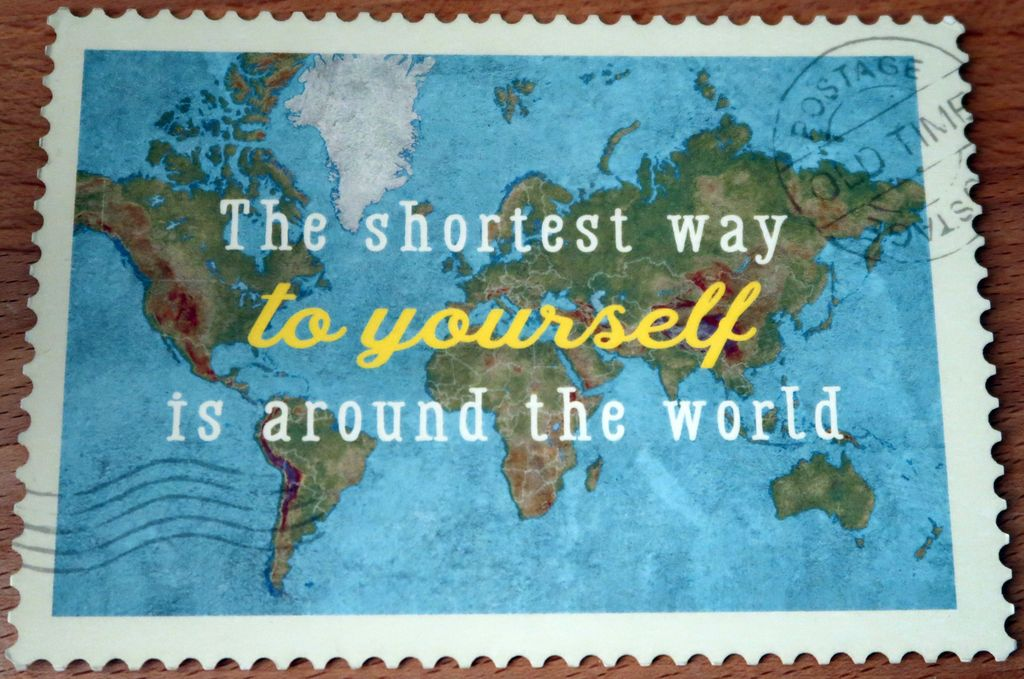
\includegraphics{images/world_postcard.jpg}
\caption{Merci à Marie-Christine pour cette carte postale qui incarne à
merveille l'esprit du voyage...}
\end{figure}

D'ici là, on vous laisse avec deux belles citations avant d'entamer
notre voyage à travers l'espace et à travers le temps :

\begin{quote}
Nous n'aurons de cesse d'explorer et la fin de toutes nos explorations
sera de revenir à l'endroit d'où nous sommes partis et de connaître le
lieu pour la première fois.
\end{quote}

\emph{T. S. Eliot,
\href{https://www.franceinter.fr/emissions/sur-les-epaules-de-darwin/sur-les-epaules-de-darwin-21-avril-2018}{cité
par Jean Claude Ameisen}}

\begin{quote}
"Vous avez longtemps voyagé", dit le Simurgh à ses sujets les oiseaux,
lorsqu'ils le découvrent enfin après une très longue quête, "vous avez
cru parfois vous perdre, mais vous ne vous êtes pas quittés. C'est vous
que vous avez retrouvés."
\end{quote}

\emph{\href{https://fr.wikipedia.org/wiki/La_Conférence_des_oiseaux}{Mantiq
at-Tayr} (La conférence des oiseaux), Farid Al-Din Attar,
\href{https://www.franceinter.fr/emissions/sur-les-epaules-de-darwin/sur-les-epaules-de-darwin-21-avril-2018}{cité
par Jean Claude Ameisen}}

\emph{Elida et Florian}

\hypertarget{la-photographie-en-voyage-un-muxe9tier}{%
\section{La photographie en voyage, un métier
?}\label{la-photographie-en-voyage-un-muxe9tier}}

\emph{Mardi 01 mai 2018}

A l'approche du voyage, nous avons acheté un appareil photo. Un Canon
PowerShot G7X Mark II, vivement recommandé par Pierre.

\begin{figure}
\centering
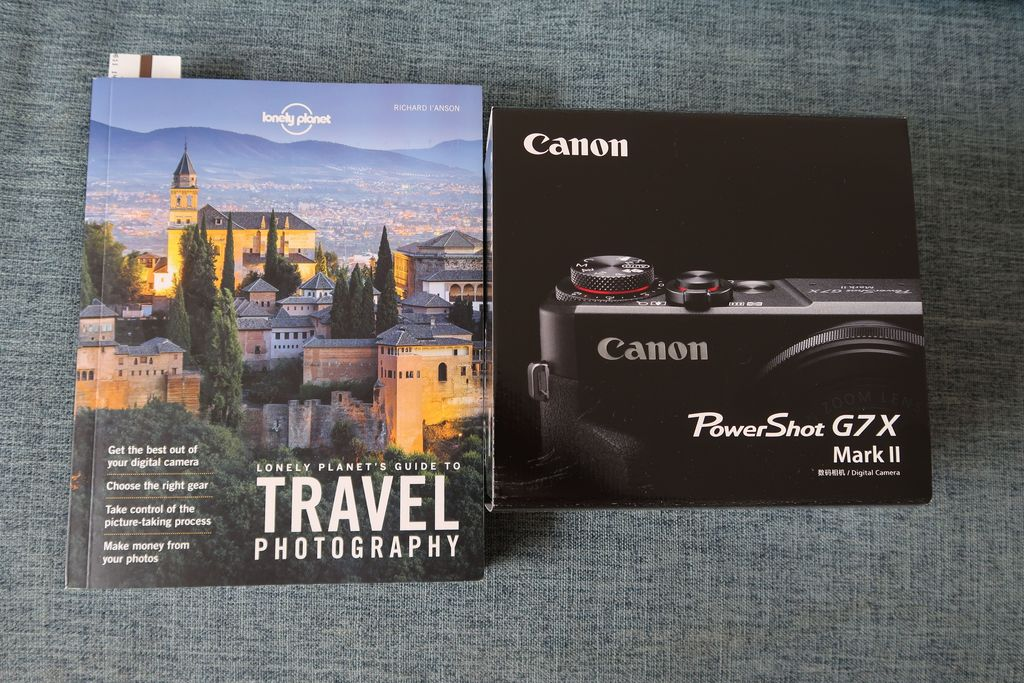
\includegraphics{images/appareil_photo_canon_g7x.JPG}
\caption{La boîte de l'appareil et le livre prêté par Ruocong pour
commencer à appréhender la thématique.}
\end{figure}

L'idée que je m'étais faite est que lorsqu'on est équipé d'un bon
appareil, on fait facilement des bonnes photos. Après quelques semaines
de pratique, je me rends bien compte que ce n'est que la partie émergée
de l'iceberg. On ne devient pas photographe en un jour.

Qu'à celà ne tienne, vous trouverez ci-dessous quelques exemples de
photos prises durant les dernières semaines avec ce bel appareil photo.
Ceci me permet également de tester l'intégration d'une gallerie photo
cliquable dans les articles de blog.

\emph{Florian}

\hypertarget{jour-j-faire-le-pont-entre-loccident-et-lorient}{%
\section{Jour J : faire le pont entre l'Occident et
l'Orient}\label{jour-j-faire-le-pont-entre-loccident-et-lorient}}

\emph{Jeudi 03 mai 2018}

Ca y est ! Après les derniers préparatifs (sportifs), nous avons laissé
derrière nous notre chez-nous. Le Liban nous attend pour le début de ce
périple.

\begin{figure}
\centering
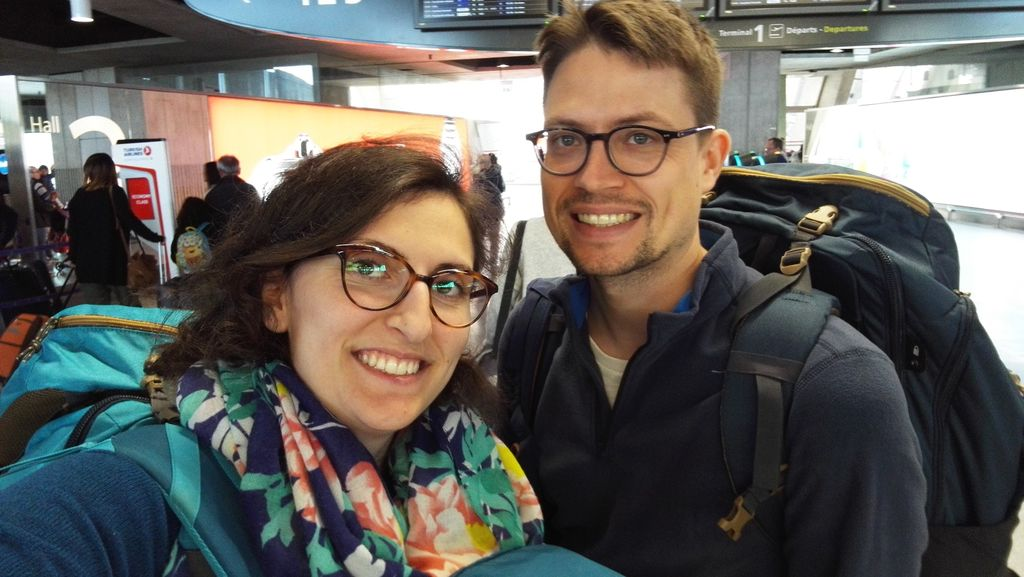
\includegraphics{images/20180503_depart.jpg}
\caption{Selfie-sac à dos de rigueur.}
\end{figure}

Est-ce qu'on réalise ce qui nous arrive ? Pas vraiment. Est-ce qu'on est
stressés ? Un peu. Une chose est sûre : on est contents :D

\begin{figure}
\centering
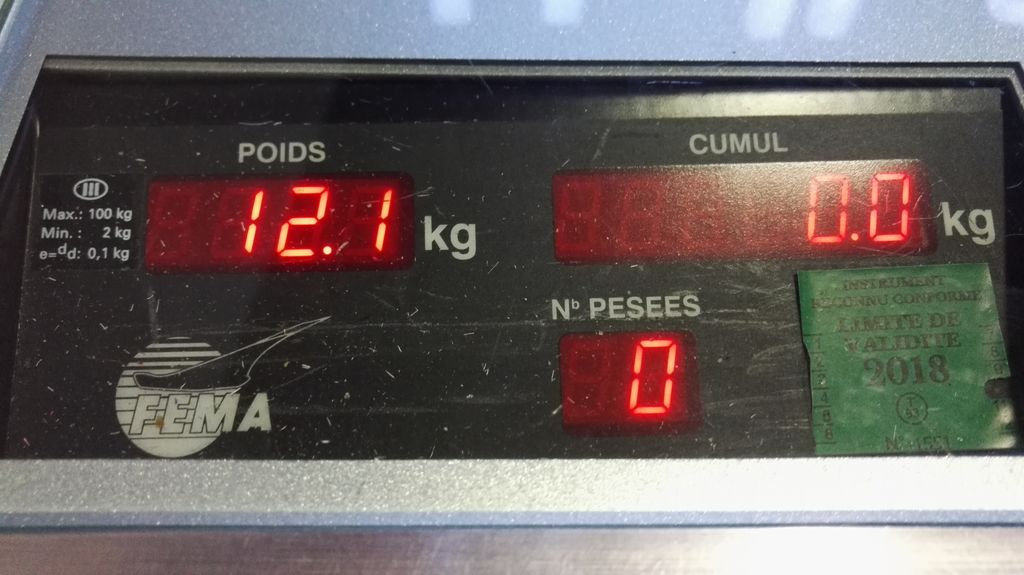
\includegraphics{images/20180503_Elida_sac.jpg}
\caption{Pour ceux qui n'y croyaient pas : elle l'a fait (ou presque...
aïe les 100 grammes de trop !).}
\end{figure}

\begin{figure}
\centering
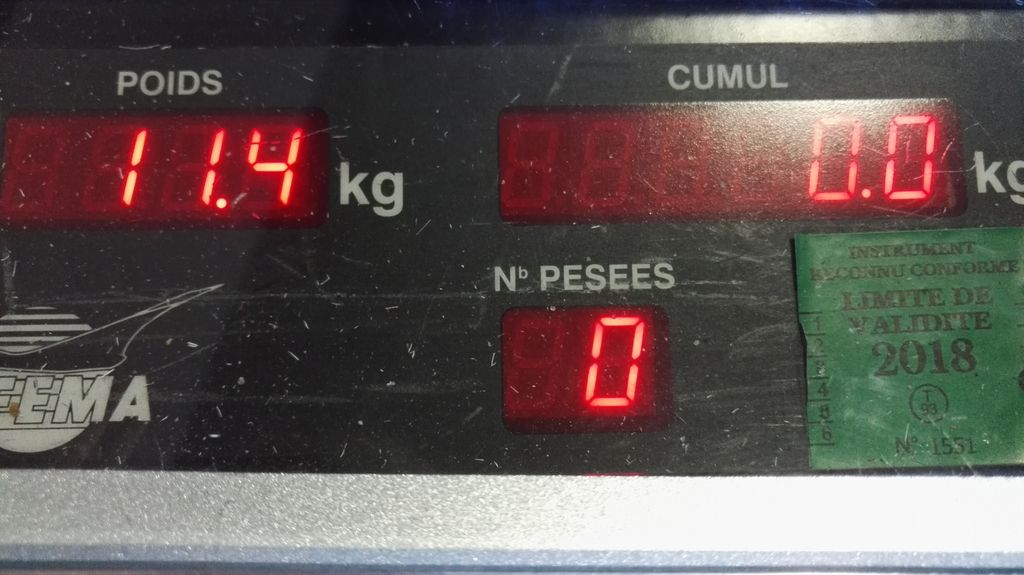
\includegraphics{images/20180503_Florian_sac.jpg}
\caption{Florian 1 - Elida 0.}
\end{figure}

Et devinez d'où on écrit ce billet ? Istanbul, première escale d'une
longue série. On fait pas mieux comme transition entre les continents !

\begin{figure}
\centering
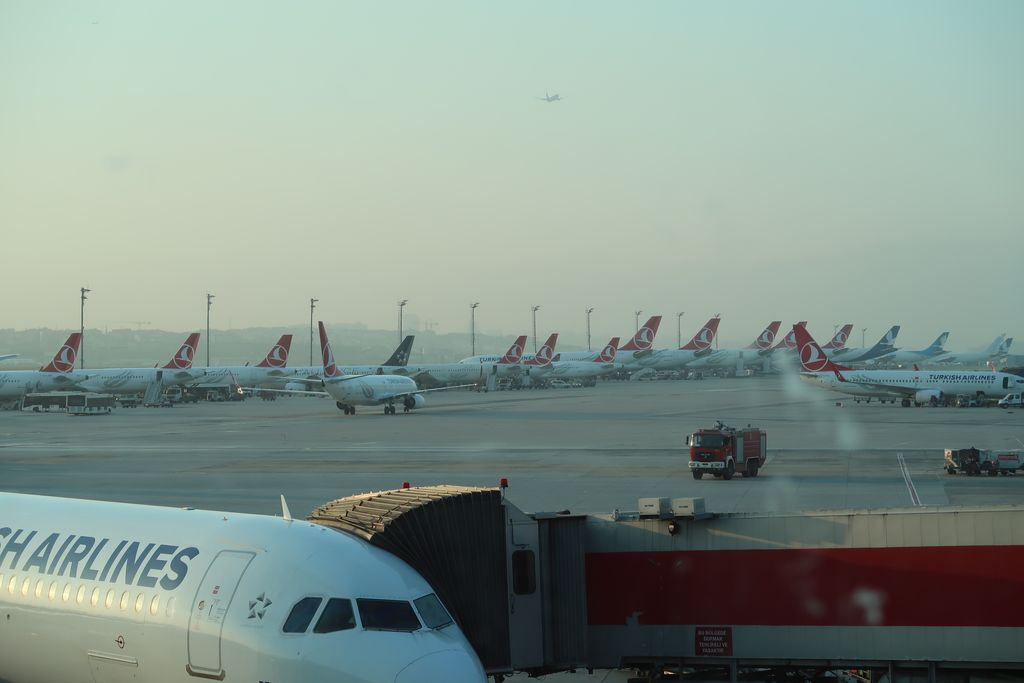
\includegraphics{images/20180503_Escale_Istanbul.JPG}
\caption{Le soleil se couche maintenant sur l'aéroport d'Istanbul (et
Flo ne rate pas une occasion de s'entraîner avec l'appareil photo ;) ).}
\end{figure}

Vite, on embarque. A très vite !

\emph{Elida et Florian}

\hypertarget{le-bonjour-du-village}{%
\section{Le bonjour du village !}\label{le-bonjour-du-village}}

\emph{Dimanche 06 mai 2018}

Les premières impressions du Liban (by Flo) :

\begin{itemize}
\tightlist
\item
  il fait chaud
\item
  il y a des voitures partout, notamment des SUV, et ça klaxonne pour
  tout et pour rien
\item
  ça sent la pollution dans la rue
\item
  on s'arrête régulièrement à des checkpoints militaires sur la route,
  plus généralement on note l'omniprésence de militaires
\item
  on se fait réveiller dès 5 heures du matin par des enfants qui jouent
  au foot dans la rue ou par la douce voix de l'épicier d'en face qui
  s'énerve sur tout le monde
\item
  c'est plein d'affiches politiques avec les têtes des candidats (le
  concours "ma binette partout"), ce qui s'explique par la tenue des
  élections législatives aujourd'hui
\end{itemize}

\begin{figure}
\centering
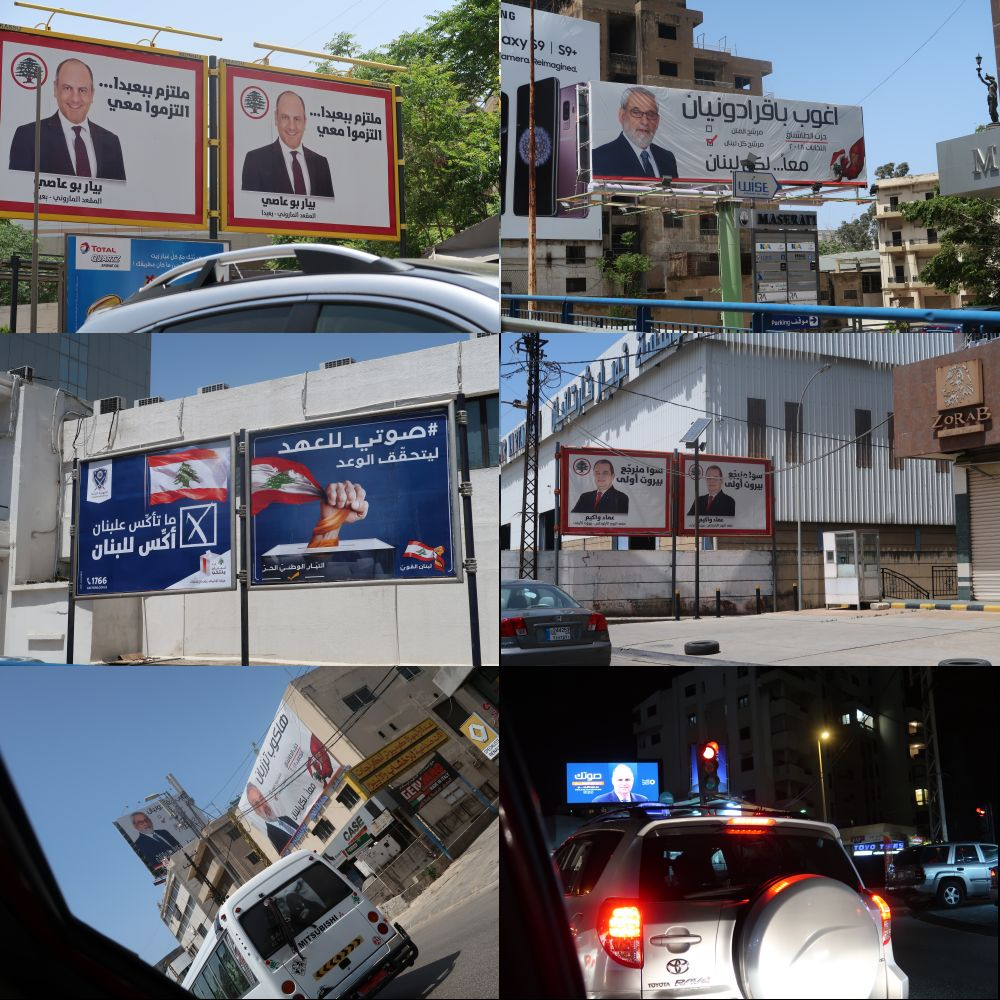
\includegraphics{images/20180506_politique.jpg}
\caption{Un échantillon d'affiches électorales libanaises.}
\end{figure}

Pour ne pas déséquilibrer le tableau, il faut rajouter deux choses : la
nourriture, qui est délicieuse (petit barbecue sur le toit pour nous
recevoir), et l'accueil adorable qui nous est reservé par la famille
d'Elida. De quoi envisager sereinement les prochains jours.

\begin{figure}
\centering
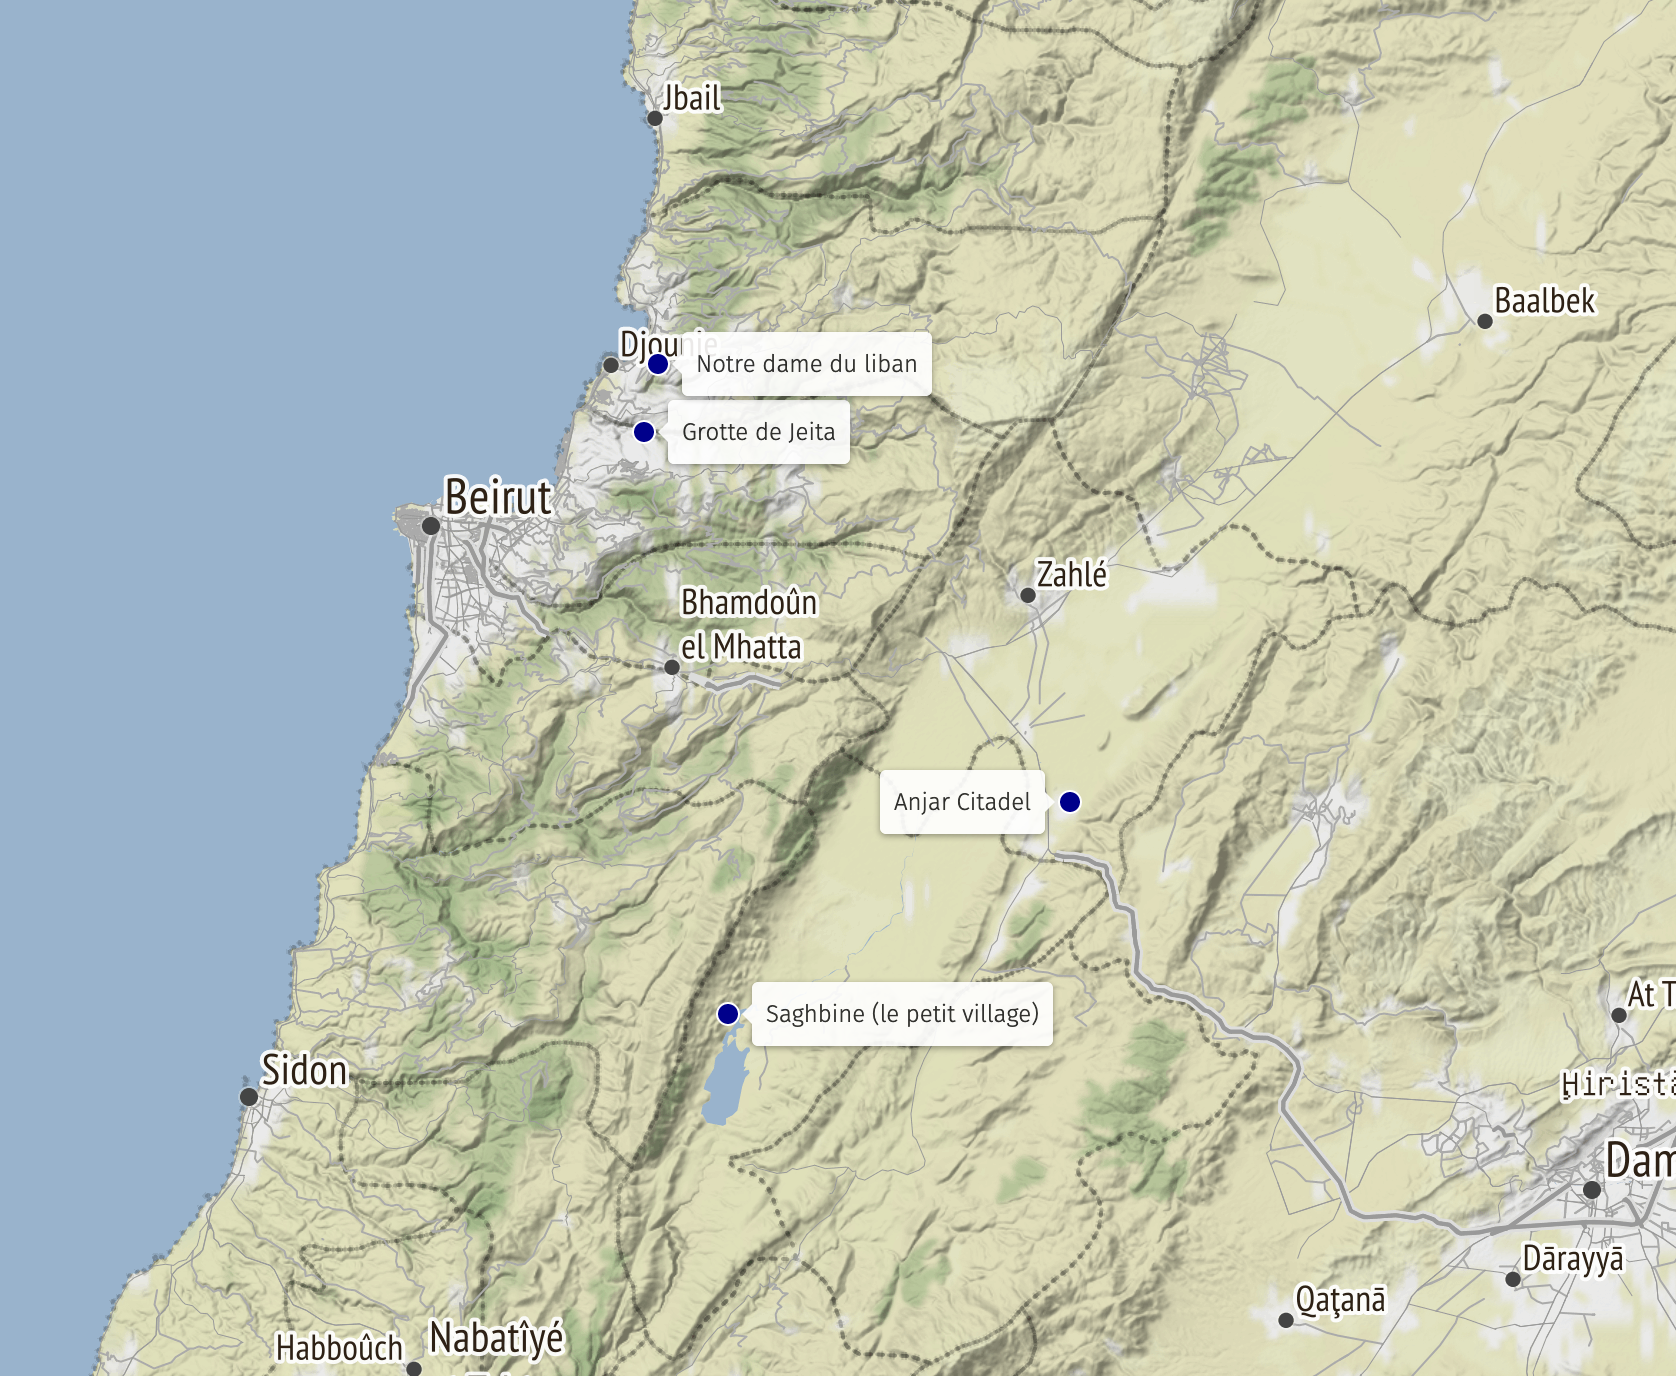
\includegraphics{maps/Liban1.png}
\end{figure}

Nous avons passé deux jours à Beyrouth, ce qui nous a donné
l'opportunité de commencer les visites au pas de course : les grottes de
Jeita, Notre Dame du Liban (NDDL pour ceux qui connaissent), le port de
Byblos.

\begin{figure}
\centering
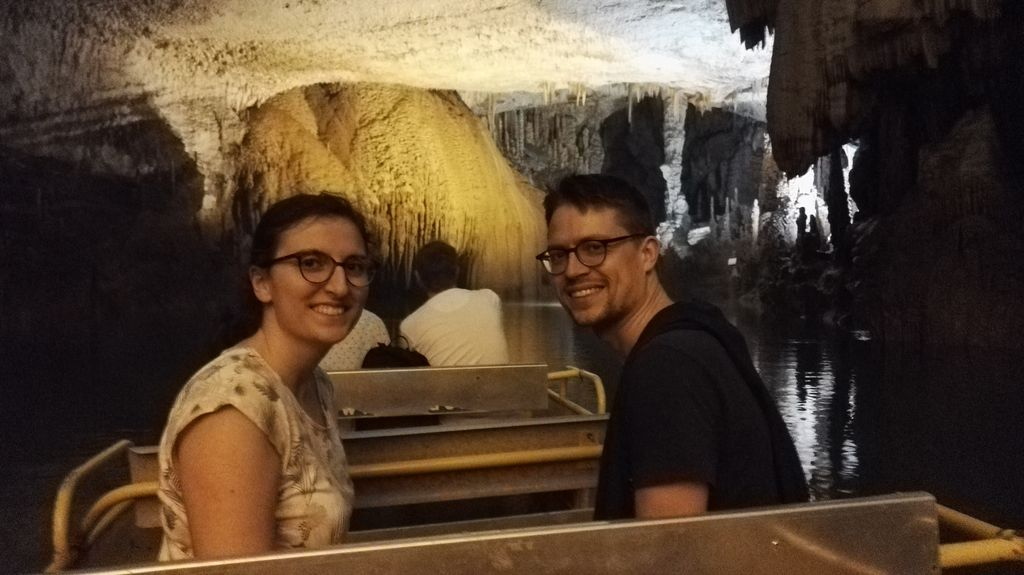
\includegraphics{images/20180506_Jeita.jpg}
\caption{Les grottes de Jeita, impressionnantes (photo volée exclusive,
bakchiche à la clé pour braver l'interdiction de photographier, on se
fait vite aux coutumes locales ;) )}
\end{figure}

Nous sommes maintenant à Saghbine, un petit village de la Bekaa de
l'ouest, une vallée coincée entre la chaîne montagneuse du mont Liban et
celle de l'anti-Liban (en face, quoi \^{}\^{}). Sur le chemin, nous
avons fait un détour par la ville d'Anjar (voir les photos de ruines
Omeyyades dans le style byzantin ci-dessous).

Ambiance politique aujourd'hui, on reste à l'écart et on vous tient au
courant !

\emph{Florian et Elida}

\hypertarget{commentaires}{%
\subsection{Commentaires}\label{commentaires}}

\begin{itemize}
\item
  François Baqué, \emph{2018-05-08 06h57}

  Bonjour depuis la Provence où la météo reste bien variable et
  fraiche... mois de mai hyper calme avec tous nos ponts et viaducs...\\
  Merci pour votre reportage libanais, au pays des cèdres majestueux et
  millénaires.\\
  Irez-vous à Byblos ? Ruines entremêlées sur 2000 ans d'histoire : des
  phéniciens aux croisés puis aux temps modernes !\\
  Vous êtes au cœur de l'origine de notre civilisation méditerranéenne :
  le barycentre (on reste dans les maths ?) de la culture mondiale
  actuelle (hors Chine : chaque chose en son temps).\\
  A très bientôt.\\
  François
\item
  Florian LB, \emph{2018-05-09 09h43}

  Bonjour François, merci pour ton message. Nous sommes passés en coup
  de vent à Byblos, mais nous y retournerons sans doute. Effectivement,
  les traces historiques sont très nombreuses au Liban et elles
  s'étalent sur des centaines et des centaines d'années, à ne plus
  savoir quelle époque on est en train de regarder. Concernant la météo,
  elle s'est nettement rafraîchie dans la vallée de la Bekaa depuis les
  lignes écrites ci-dessus...\\
  A bientôt,\\
  Florian
\end{itemize}

\hypertarget{des-uxe9lections...uxe0-la-foruxeat-des-cuxe8dres}{%
\section{Des élections...à la forêt des
Cèdres}\label{des-uxe9lections...uxe0-la-foruxeat-des-cuxe8dres}}

\emph{Jeudi 17 mai 2018}

\begin{figure}
\centering
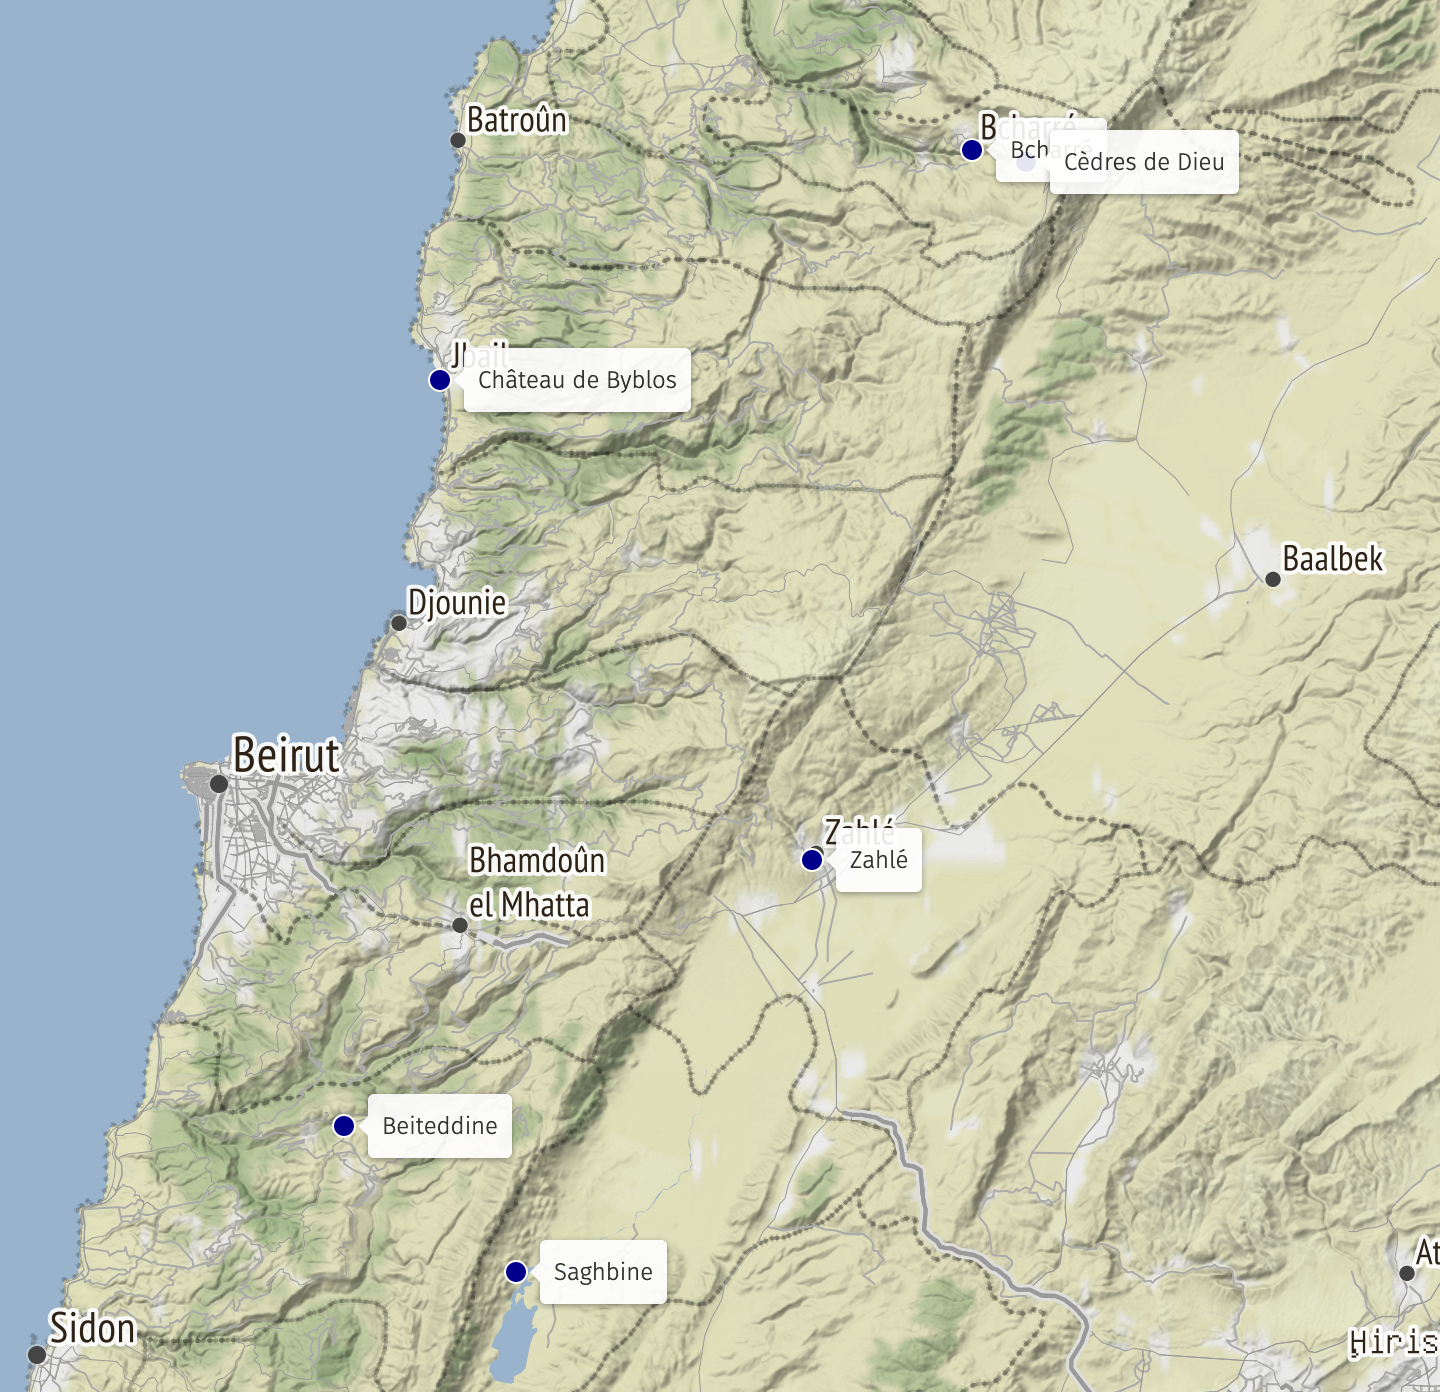
\includegraphics{maps/Liban2.png}
\end{figure}

Dans un climat bien chargé, autant politiquement que météorologiquement
(des pluies battantes et orages en mai pendant plusieurs jours, tous les
libanais nous ont juré n'avoir jamais vu ça...), nous avons tout de même
continué nos explorations diverses. A commencer par les bureaux de vote
! Les élections législatives qui se sont tenues sont les premières
depuis 9 ans. Les gens étaient globalement partagés, entre la motivation
de s'exprimer par les urnes et le côté défaitiste devant la corruption
(on a entendu des promesses d'achats de voix jusqu'à 2000 dollars !) et
les tricheries, qui ont malheureusement bien eu lieu. J'ai choisi mon
camp et je suis allée voter ! (et mon candidat, malgré un score ridicule
dans le village, a bien été élu dans la circonscription !
\textbackslash{}o/). Outre l'omniprésence militaire autour et dans les
bureaux de vote, voir les listes électorales triées par religion fait
toujours son petit effet... Bref, une fois les différents entre
partisans politiques réglés (en gros, une fois que tout le monde s'est
bien foutu sur la tronche), on a pu reprendre le fil de nos excursions.

Nous avons parcouru la vallée de la Bekaa, coincée entre deux chaînes
montagneuses et traversée par le fleuve Litani, retenu par le barrage de
Qaraoun.

\begin{figure}
\centering
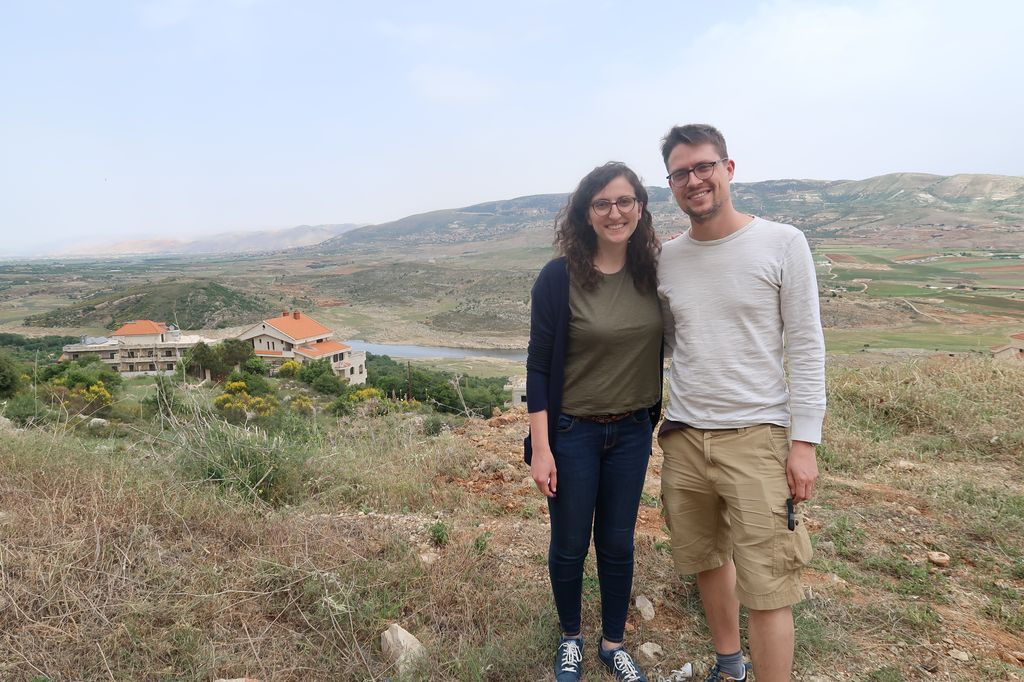
\includegraphics{images/20180517_bekaa.jpg}
\caption{Vallée de la Bekaa après le vote.}
\end{figure}

Un de mes cousins nous a ensuite emmenés vers le palais de Beiteddine,
en passant par la forêt des Cèdres du Chouf (qu'on a pas vraiment vue
-private lebanese joke inside- du fait d'une météo peu clémente dont on
va continuer à se plaindre un peu).

Le palais de Beiteddine a été construit au 19ème siècle pour le grand
émir du Liban. Il est actuellement utilisé comme résidence d'été par le
président de la République, et tous les étés pour le festival de musique
et de danse.

\begin{figure}
\centering
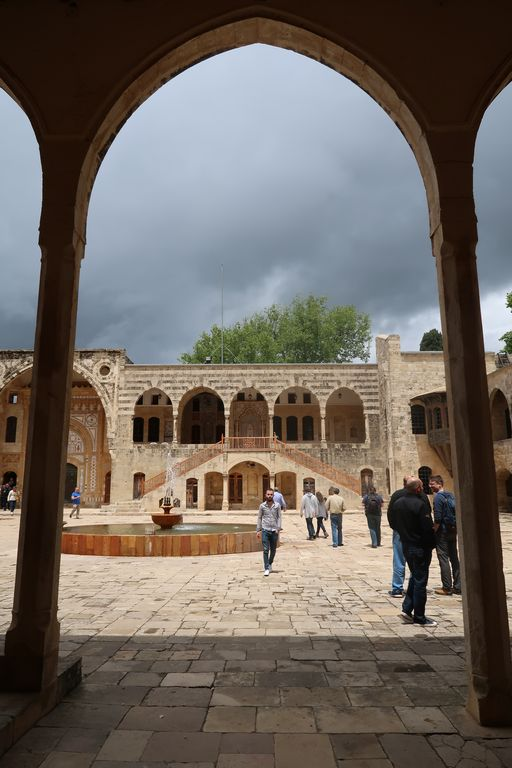
\includegraphics{images/20180517_beiteddine.jpg}
\caption{Le palais, de style ottoman.}
\end{figure}

Zahlé est la capitale du gouvernorat de la Bekaa. Nous avons grimpé les
240 marches de Notre Dame de Zahlé pour admirer la vue panoramique sur
la ville et la vallée. Après un bon taouk (article gastronomique dédié à
venir), nous avons continué nos explorations jusqu'aux caves de Ksara,
où des centaines de tonneaux de vin sont entreposés dans des galeries
datant de l'époque romaine (et où l'on a dégusté le vin produit sur
place).

\begin{figure}
\centering
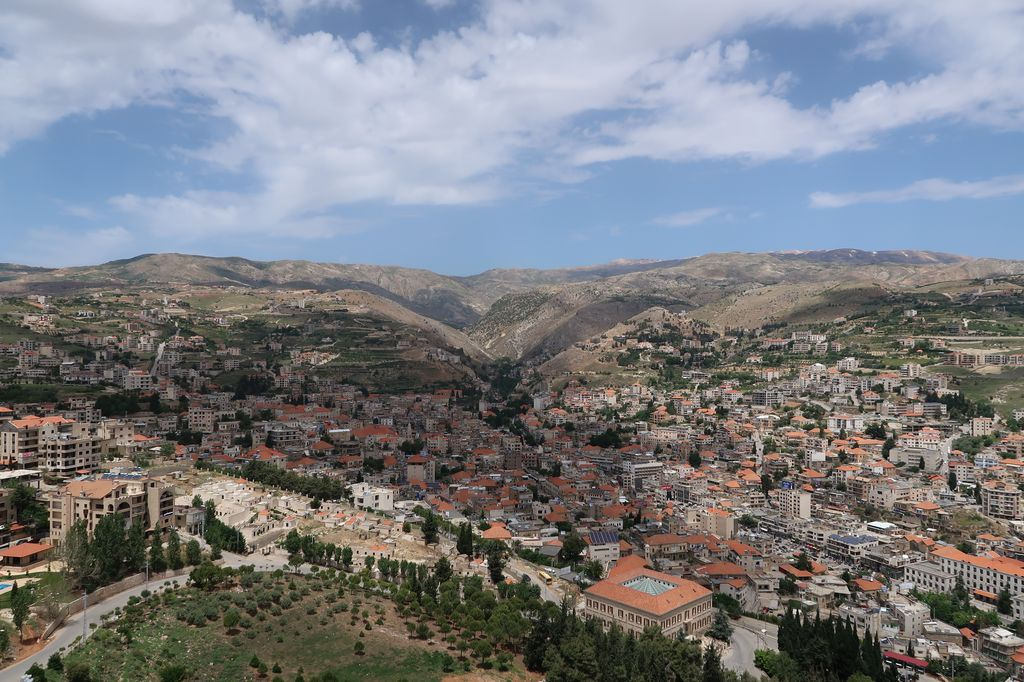
\includegraphics{images/20180517_zahle.jpg}
\caption{Vue panoramique de Zahle.}
\end{figure}

Byblos, que nous avions déjà exploré de nuit la semaine précédente,
mérite le détour de jour pour la visite des vestiges près du port. Le
fort date de l'époque des croisés, mais repose en fait sur les strates
d'occupation plus ancienne (Byblos prétend au titre de ville la plus
vieille du monde). Dans la lumière du jour déclinant, on prend la mesure
de la beauté du site.

\begin{figure}
\centering
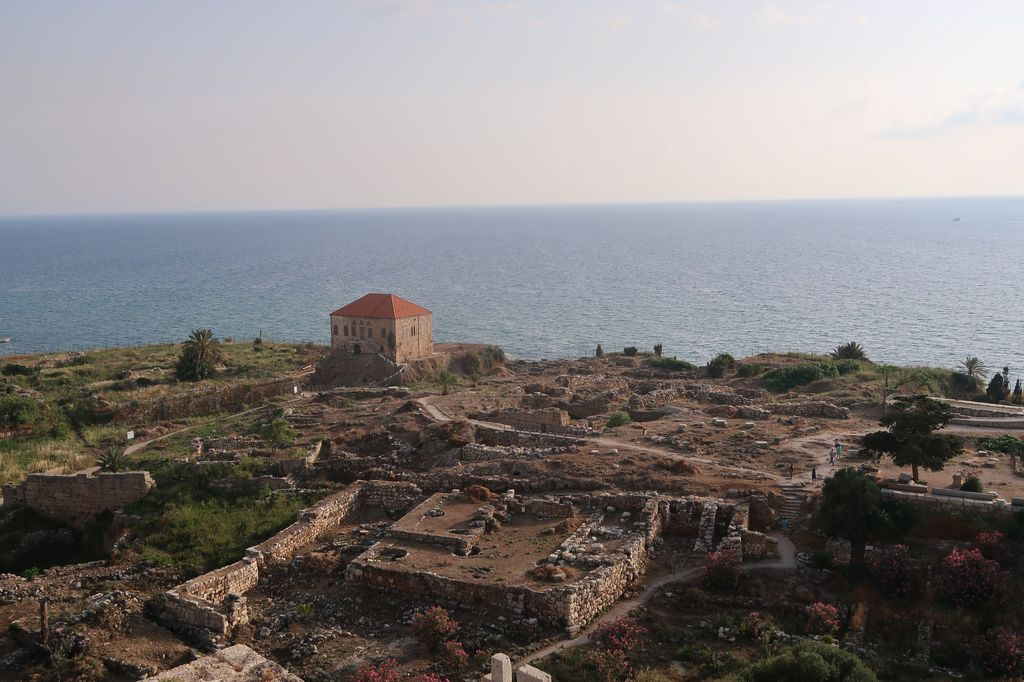
\includegraphics{images/20180517_byblos.jpg}
\caption{Le site de Byblos, au bord de la mer.}
\end{figure}

Premières aventures au volant (et ce n'est pas une mince affaire, vu
l'absence totale de règles de la route "ici, la priorité est au plus
brave", "tu conduis comme tu le sens, et ça marche bien comme ça"), Flo
nous a conduit dans le Nord du pays, jusqu'à une autre forêt de cèdres,
celle de Bcharré. Cette fois nous avons un temps agréable qui nous
permet d'admirer ces colosses parfois millénaires, et dont l'utilisation
du bois est attestée depuis la Mésopotamie... Une balade très agréable,
qui se poursuit à Bcharré où nous visitons le musée de Khalil Gibran
(pour ceux qui ne connaissent pas, lire \emph{Le Prophète} est un must
!), où sont exposées les nombreuses peintures de l'artiste. Cette visite
nous a refait plonger dans ses écrits dont l'extrait suivant nous avait
particulièrement parlé avant notre départ :

\begin{quote}
Me voici prêt à partir, et mon impatience aux voiles déployées attend le
vent. Je ne respirerai qu'une dernière bouffée de cet air calme, je ne
jetterai qu'un dernier regard d'amour en arrière, et alors je serai au
milieu de vous, un navigant parmi les navigants.
\end{quote}

C'est les yeux pleins de ces paysages variés (et les ventres bien
pleins) que la suite se prépare...

\textbf{Bonus demandé par Thibaud : prendre la voiture au Liban.}

Je suis désolé, votre navigateur ne supporte pas les vidéos HTML5 au
format WebM avec VP8 ni au format MP4 avec H.264.

\emph{Elida et Florian}

\hypertarget{tripoli-beyrouth-qadisha-sauxefda}{%
\section{Tripoli, Beyrouth, Qadisha,
Saïda}\label{tripoli-beyrouth-qadisha-sauxefda}}

\emph{Lundi 21 mai 2018}

\hypertarget{mapid}{}

La semaine dernière, nous avons poursuivi nos excursions depuis
Beyrouth.

La première a été la ville de Tripoli, au nord du Liban. On y trouve le
château Saint Gilles, initialement construit par les croisés, en très
bon état. Situé au sommet de la colline, il propose une belle vue sur la
ville et la côte. Nous y avons également visité un hammam vieux de 800
ans et restauré depuis sa fermeture dans les années 1970. Après avoir
traversé le dédale des ruelles du vieux souk, nous avons fini la journée
dans une des institutions de la ville : la pâtisserie Hallab où on a pu
déguster des douceurs locales...

\begin{figure}
\centering
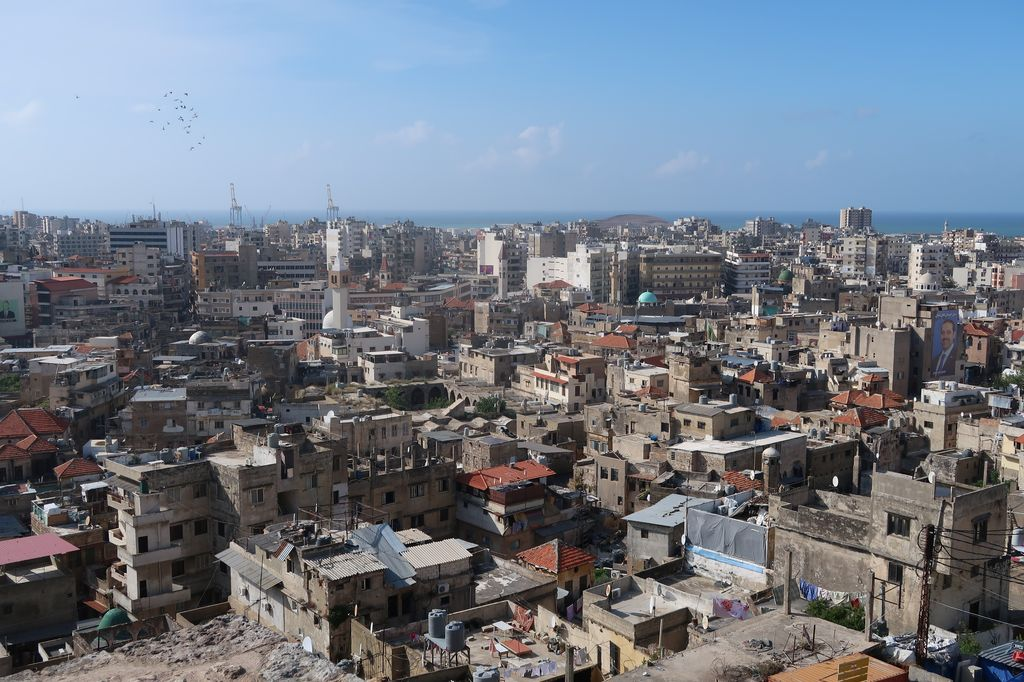
\includegraphics{images/20180521_tripoli.JPG}
\caption{Vue sur Tripoli depuis le château Saint Gilles.}
\end{figure}

Nous avons profité d'avoir un gîte à Beyrouth pour nous promener durant
plusieurs journées dans la ville. Que retenir de la capitale du Liban ?
Pour moi, c'est un mélange étonnant de routes serrées et de ruelles, de
voitures trop nombreuses, de promenades en bord de mer, d'immeubles
abandonnés, d'impacts de balles rebouchés ou non sur les façades, de
blocs d'appartement modernes et de villas somptueuses. On peut noter que
le centre ville a été reconstruit à neuf après les années de guerre
civile (1975 - 1990) et a une allure atypique et très propre de ce fait.
Nous avons également profité de l'agréable musée national qui nous a
permis de couvrir du regard les millénaires d'histoire du Liban, et du
musée de l'American University of Beirut qui est venu compléter cette
parenthèse dans le passé.

\begin{figure}
\centering
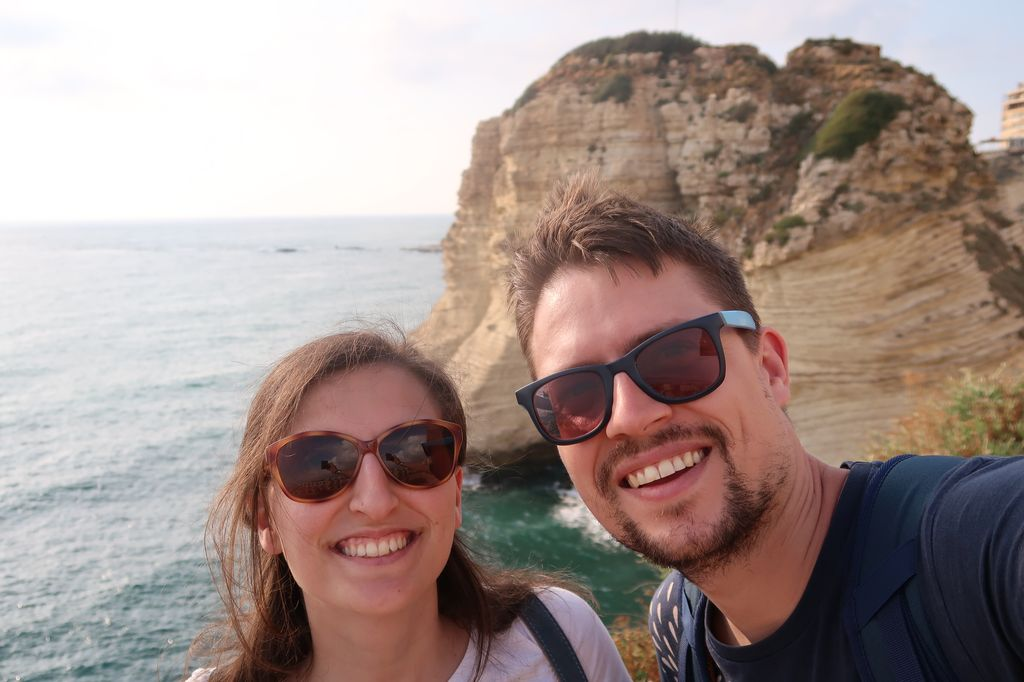
\includegraphics{images/20180521_Rausche.JPG}
\caption{Selfie devant l'une des vues touristiques de Beyrouth : le
rocher aux pigeons.}
\end{figure}

L'un des moments les plus agréables de cette semaine a été l'excursion
dans la "vallée sainte de Qadisha". Cette vallée porte une longue
histoire religieuse, ayant été tour à tour refuge de chrétiens
persécutés ou d'ermites, avec de nombreuses caves creusées dans la roche
ainsi que de nombreux monastères construits au fil des quinze derniers
siècles. Nous avons eu la chance de la visiter en présence d'un guide
français, "Monsieur Yves", qui nous a plus d'une fois surpris par la
profondeur de son érudition et sa connaissance pointue du lieu. Il nous
a emmené randonner dans la vallée, jusqu'à Hawqa où vit actuellement un
ermite, puis jusqu'au couvent de Qannoubine où vivent encore deux
religieuses. La marche est raide mais très belle et impressionnante. On
a du mal à imaginer les conditions d'accès à ces sanctuaires il y a
plusieurs centaines d'années, sans équipement si aménagements du
sentier.

\begin{figure}
\centering
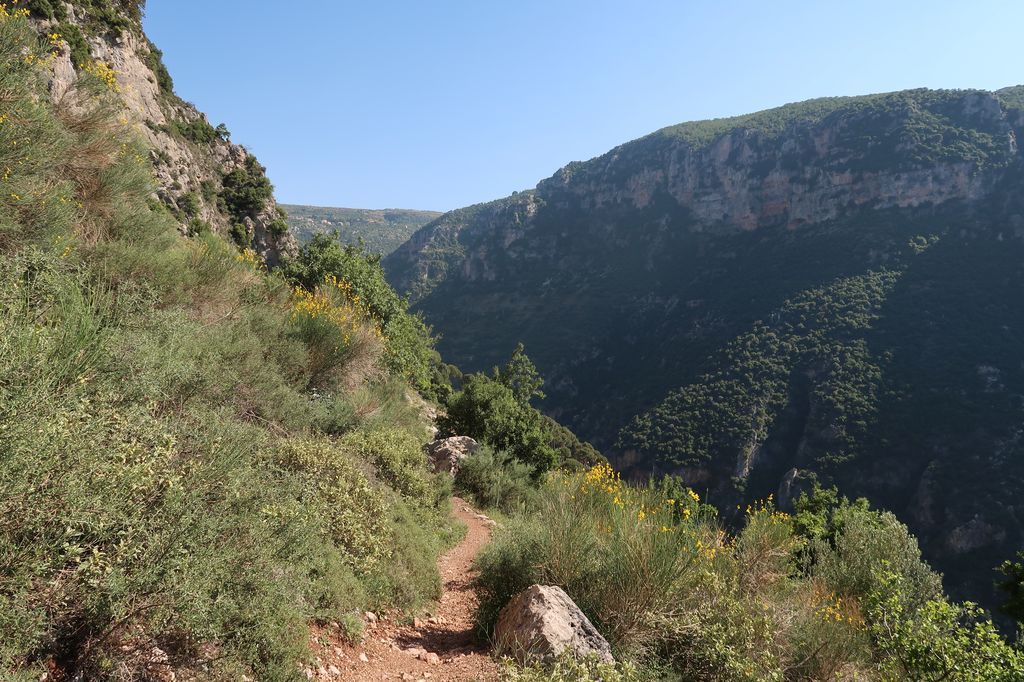
\includegraphics{images/20180521_qadisha.JPG}
\caption{La végétation dans la vallée de Qadisha.}
\end{figure}

Notre dernière excursion de la semaine nous a amené à Saïda, au sud de
Beyrouth. A ce sujet, il est intéressant de noter que l'on se déplace
facilement en bus au Liban, mais avec un certain nombre de différences
par rapport aux bus que j'ai l'habitude de prendre : absence d'arrêts
officiels (on peut monter à partir du moment où on fait signe au
chauffeur, y compris sur la bande d'arrêt d'urgence de l'autoroute), pas
d'horaires définis, prix non affichés... A Saïda, nous avons trouvé une
petite ville avec un souk typique, une citadelle marine de l'époque des
croisés (encore eux !) ainsi qu'un musée du savon plutôt bien fait. Note
pour plus tard : visiter une ville à prédominance musulmane le premier
jour du Ramadan n'est pas une mince affaire lorsqu'il s'agit de se
restaurer ;)

Enfin, nous avons également ajouté à la liste des sanctuaires visités
celui de Saint Charbel, l'un des saints libanais les plus connus.

Bon, il commence à faire un peu trop chaud à Beyrouth, on retourne plus
en altitude pour nos derniers jours ici :)

\emph{Florian et Elida}

\hypertarget{manger-au-liban}{%
\section{Manger au Liban}\label{manger-au-liban}}

\emph{Mercredi 23 mai 2018}

Comme je l'ai déjà écrit dans le premier billet sur le Liban, nous avons
été accueilli de manière extrêmement généreuse par la famille d'Elida.
Tout le monde s'occupe de nous, nous propose des excursions, demande
comment je trouve le Liban et... nous invite à manger. Cela se traduit
principalement par deux choses : la commande d'un nombre extraordinaire
de plats, bien au-delà du raisonnable, et le fait qu'on ressort de table
après plusieures heures en n'ayant plus du tout faim :D

\begin{figure}
\centering
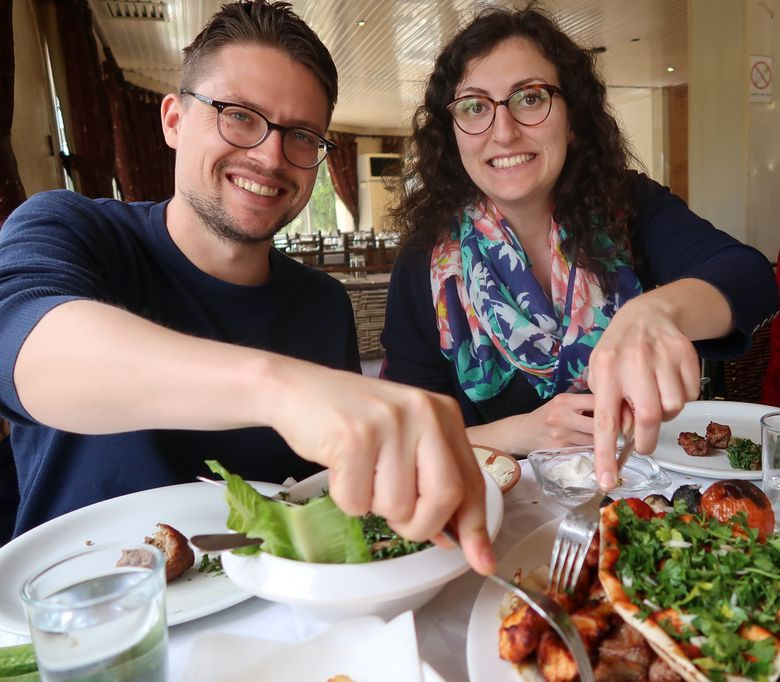
\includegraphics{images/20180523_manger.JPG}
\caption{Exemple de festin sur fond de gastronomes heureux.}
\end{figure}

Le déroulement d'un repas peut être décrit par la séquence suivante :

\begin{itemize}
\tightlist
\item
  on amène des petites choses à grignoter à la table (par exemple :
  olives, amandes vertes qu'on mange en entier, petits pois,
  cacahouètes)
\item
  le serveur demande "Fattoush ou Tabbouleh ?" et prend la commande des
  mezzés et des plats
\item
  le serveur sert le Fattoush / Tabbouleh, puis les mezzés arrivent et
  on en mange avec du pain libanais qu'on déchire pour former des petits
  récipients pour aller "pêcher" du Hommous et du Labneh
\item
  on n'a plus faim car tout est très bon et on a eu envie de tout goûter
\item
  les grillades (kefta, taouk de poulet, brochettes de boeuf) arrivent,
  on est surpris car on ne s'y attendait plus, et on en mange même si on
  a plus faim
\item
  on n'a vraiment plus faim
\item
  on passe au dessert (fruits frais, gâteau d'anniversaire ou de baptême
  s'il y a lieu, gâteaux pleins de sirop de sucre)
\end{itemize}

Optionnellement, on peut bien entendu commander un narguilé (qu'on
appelle d'ailleurs arguilé ici) que l'on "déguste" au fil du repas.

On peut noter que par rapport au repas français traditionnel, le repas
libanais ne s'accompagne pas forcément d'un café à la fin (je me suis
rendu compte qu'on sert le café "à la turque" à n'importe quelle heure
de la journée, et qu'il est généralement moins fort que le café que l'on
a coutume de boire en France).

Concernant les boissons alcoolisées, l'Arak occupe une place de premier
choix sur la table libanaise. Qu'il soit fait maison ou pas, on en
rencontre bien plus souvent que le vin de nos contrées.

Vous l'aurez compris, on mange bien au Liban.

Malheureusement, ceci m'amène au revers de la médaille : au restaurant,
ce qui est commandé mais n'a pas pu être mangé par les convives finit...
à la poubelle ! La culture de l'hospitalité prescrit un festin, mais ne
prévoit pas (encore ?) de garder les restes et de les ramener à la
maison.

Allez, on vous laisse saliver avec nos photos de repas libanais !

\emph{Florian}

\hypertarget{baalbeck-au-revoir-liban}{%
\section{Baalbeck \& au revoir, Liban
!}\label{baalbeck-au-revoir-liban}}

\emph{Vendredi 25 mai 2018}

Le point d'orgue de nos derniers jours au Liban a été la visite des
ruines de Baalbeck. Ces ruines, dont l'origine remonte aux romains, sont
extrêmement impressionnantes. Dans les presques vingt siècles qui ont
suivis leur construction, elles ont été réutilisées par les différents
peuples qui ont habité cette région. Jusqu'à aujourd'hui, puisque le
site est utilisé pour accueillir le festival international de musique de
Baalbeck.

\begin{figure}
\centering
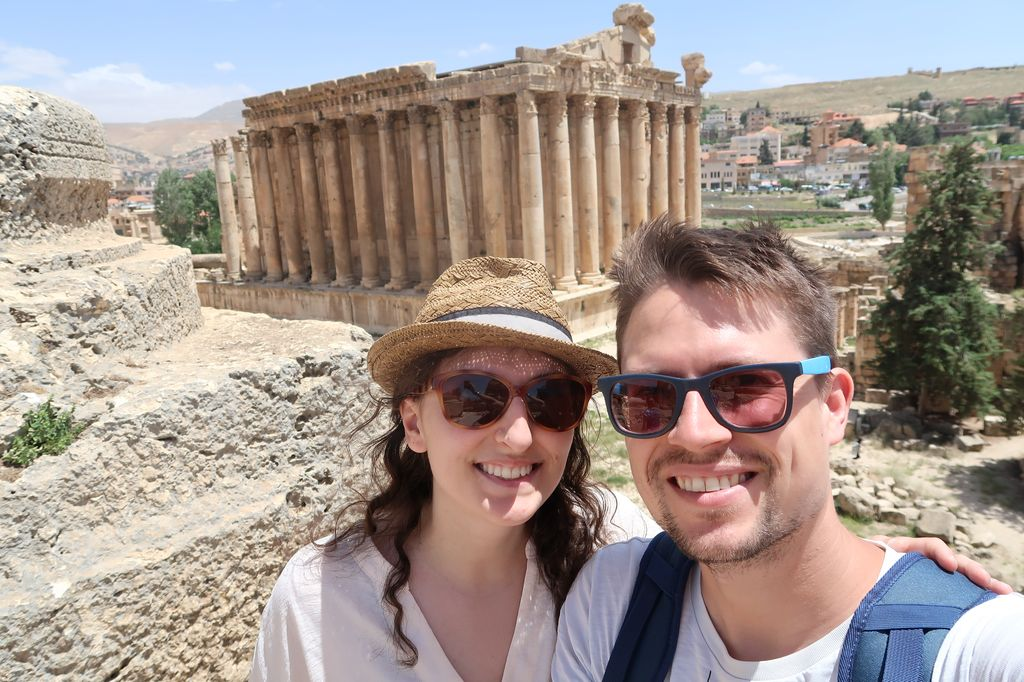
\includegraphics{images/20180525_baalbeck.JPG}
\caption{La vue sur le temple de Bacchus.}
\end{figure}

Ce qui frappe lorsqu'on visite le site, c'est l'ampleur des
installations romaines, construites sur plusieurs siècles. On distingue
l'édifice principal ("temple de Jupiter") dont les six colonnes
d'environ 20 mètres sont emblématiques et le temple dit de Bacchus, le
mieux conservé. Les pierres sont si grandes qu'on se pose immédiatement
la question des techniques de construction utilisées. Cela dit, il
semblerait qu'il n'y ait pas besoin d'invoquer de forces
extra-terrestres à cet endroit, mais bien la présence de nombreux bras,
boeufs et de systèmes de poulie comme expliqué dans
\href{http://www.persee.fr/doc/syria_0039-7946_1977_num_54_1_6623}{cet
article de 1977}.

Les derniers jours au Liban, nous les avons passés à Saghbine, à l'abri
du soleil qui tape de plus en plus fort et à explorer quelques endroits
alentours : vergers, sources et terres forestières de ce pays qui à la
belle saison regorge de fruits.

Au revoir, Liban ! Ou plutôt : à bientôt. Nous reviendrons :)

\emph{Florian et Elida}

\hypertarget{commentaires}{%
\subsection{Commentaires}\label{commentaires}}

\begin{itemize}
\item
  Pierre Guérold, \emph{2018-06-07 20h57}

  Et voilà que je me retrouve à lire un article sur le levage des
  pierres dans l'antiquité....\\
  C'est juste wahou votre voyage.\\
  Merci :)\\
  Pierre
\item
  Florian LB, \emph{2018-06-08 18h11}

  Trop cool ! Je me demandais qui allait être assez courageux pour
  cliquer sur le lien. J'ai trouvé ce sujet très intéressant, mais j'ai
  pas tout compris. Alors j'espère qu'on pourra en reparler quand on
  sera rentré ! A bientôt !
\end{itemize}

\hypertarget{proluxe9taires-de-tous-les-pays-unissez-vous}{%
\section{Prolétaires de tous les pays, unissez-vous
!}\label{proluxe9taires-de-tous-les-pays-unissez-vous}}

\emph{Dimanche 27 mai 2018}

Bonsoir à tous !

Nous sommes arrivés à Moscou vendredi.

Nous avons eu droit à un accueil formidable de la part de nos deux hôtes
russes, Stanislav et Irma, et nous sommes déjà largement promenés dans
le centre-ville de Moscou.

\begin{figure}
\centering
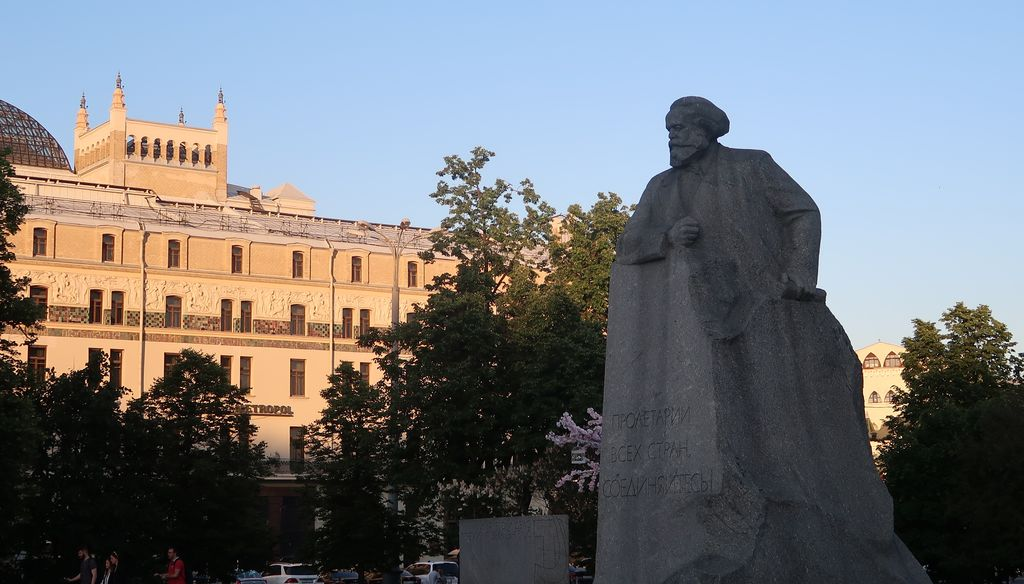
\includegraphics{images/20180527_marx.JPG}
\caption{La statue de Marx près de la place Rouge, sur le socle de
laquelle il est écrit "Prolétaires de tous les pays, unissez-vous !". Un
slogan aujourd'hui étonnant, caché en plein centre-ville.}
\end{figure}

Alors que dire, à ce stade, de nos impressions ? Je suis sous le charme
de la grande et belle ville de Moscou. Et en même temps, un mystère
demeure : c'est donc ici, le pays de Vladimir Poutine et de l'ancienne
URSS ? Mes idées reçues ne correspondent pas à la soirée quasi-estivale
que nous venons de passer avec ces groupes qui font de la musique en
plein-air et tout ce beau monde qui se promène.

Affaire à suivre !

\emph{Florian}

\hypertarget{commentaires}{%
\subsection{Commentaires}\label{commentaires}}

\begin{itemize}
\item
  Thibaud, \emph{2018-05-29 19h08}

  Dis-toi que bientôt des milliers de fan de foot vont se dire
  exactement la même chose \^{}\^{} Ce qui est très bon pour la Russie.
  Perso ça me fait plaisir !
\item
  pythux, \emph{2018-05-31 10h18}

  Pourquoi les fans de foot se diraient "prolétaires unissez-vous" ? :p
  Le foot n'intéresse pas que les prolétaires !!
\item
  Thibaud, \emph{2018-06-25 20h40}

  On voit les mecs qui ne lisent que le titre avant de filer aux
  commentaires \^{}\^{}
\item
  pythux, \emph{2018-06-25 20h44}

  Le contenu de l'article n'est qu'on prétexte ! Les commentaires, c'est
  là que tout se passe !
\item
  pythux, \emph{2018-05-31 10h25}

  On ne m'ôtera pas de l'idée, que tout ceci date de l'époque où ils
  con-solidaient une certaine idéologie en con-struisant des statues
  partout. La fameuse con-stellation de la grande URSS.
\end{itemize}

\hypertarget{crapahutages-sur-la-moscova}{%
\section{Crapahutages sur la
Moscova}\label{crapahutages-sur-la-moscova}}

\emph{Dimanche 03 juin 2018}

Nous venons de passer 6 jours à Moscou, que nous avons exploré en long,
en large, en travers, mais surtout à pied ! La marche y est très
agréable : les trottoirs sont très larges, propres, les bâtiments sont
beaux avec des bas-reliefs et des statues à tout va, et la ville est
globalement plate ce qui facilite grandement les choses :)

Comme ça risque d'être un peu long de raconter tout ce qu'on a vu et
visité, je vais plutôt vous raconter mes impressions et constats sur la
vie à Moscou. Aucune prétention de sociologie, juste des ressentis :

\begin{itemize}
\tightlist
\item
  Moscou c'est grand, pas seulement par la taille de la ville mais par
  la taille de chaque bâtiment, que ce soit la Lubjanka, le parlement,
  la bibliothèque nationale ou des immeubles de HLM, tout est démesuré.
\item
  Moscou c'est joli. Alors je pense qu'il y a un gros biais avec la
  préparation de la coupe du Monde de football qui commence dans quinze
  jours, mais on trouve partout des rues avec un toit de loupiotes, des
  arbres illuminés la nuit dans les parcs, des arcades de fleurs...
\end{itemize}

\begin{figure}
\centering
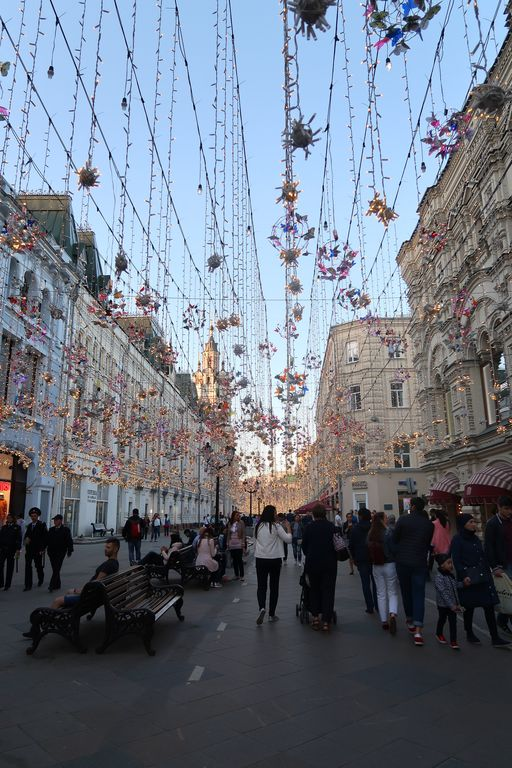
\includegraphics{images/20180603_moscou.JPG}
\caption{La rue Nikolskaya et son plafond de lumière.}
\end{figure}

\begin{itemize}
\tightlist
\item
  à propos de fleurs, si queulqu'un veut faire fortune à Moscou, ça ne
  sert à rien de se lancer dans la pétro-chimie ou dans le caviar, il
  faut faire fleuriste. Ces gens ont un truc avec les fleurs... on
  pourrait dire qu'on vit ici un bouquet à la main.
\item
  le métro est incroyable, surtout pour de bons parisiens que nous
  sommes : c'est grand, c'est propre, ça sent bon (!), et c'est surtout
  un musée à part entière, avec des stations majestueusement décorées et
  toutes différentes les unes des autres. C'est aussi très profond (les
  escalators sont vertigineux) et très bien organisé. J'imagine la tête
  des touristes moscovites à Paris quand ils prennent notre métro pour
  la première fois...
\end{itemize}

\begin{figure}
\centering
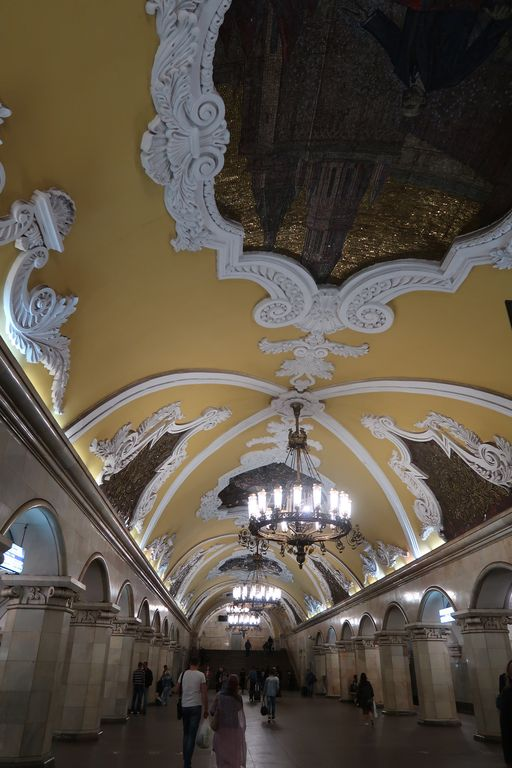
\includegraphics{images/20180603_metro.JPG}
\caption{Les stations de métro sont quasiment des oeuvres d'art !}
\end{figure}

\begin{itemize}
\tightlist
\item
  les femmes moscovites ont du style, vraiment, lookées de la tête aux
  pieds
\item
  par contre, par rapport à nos standards (encore une fois), nous
  n'avons pas trouvé les russes très polis. On ne nous a jamais, ne
  serait-ce qu'une fois, tenu la porte, les gens de l'hôtel ne m'ont
  jamais répondu quand je leur disais bonjour ni au-revoir, on se fait
  souvent bousculer (et je ne parle pas des hordes de touristes en
  groupe, c'est une autre histoire !) et on ne nous a jamais souri à une
  caisse de restaurant ou de supermarché. Heureusement qu'il y a des
  exceptions. Je pense à cette dame qui passait par là et qui, devant
  nos airs paumés nous a spontanément proposé son aide pour retrouver
  notre chemin vers la gare de Léningrad :)
\item
  et l'alphabet cyrillique, on en parle ? Un alphabet avec globalement
  des lettres qu'on connaît, mais t'as une chance sur deux pour que ça
  se prononce pas du tout comme tu crois. Donc, petit cours rapide : le
  P se prononce R, le C se prononce S, le H se prononce N, le Y se
  prononce OU, le grand B se prononce V, le petit b est en fait un grand
  B et se prononce B. Voilà, vous avez tout suivi ? Du coup, si je vous
  écris PECTOPAH, vous le prononcez...? Restaurant ! Bravo, vous êtes
  niveau 1 en cyrillique \textbackslash{}o/. Heureusement que Flo s'en
  sort bien en Russe sinon je serais perdue \^{}\^{}
\item
  dans un autre domaine, la scène musicale est super riche et très
  intéressante. Il y a des concerts de rue à tous les coins,
  généralement de bonne qualité, où les gens s'arrêtent volontiers pour
  écouter, et ça fait une super ambiance
\item
  bon, je crois qu'on parlera pas de la nourriture, les souvenirs du
  Liban sont trop frais encore, on n'est pas prêts ;)
\end{itemize}

D'ailleurs, parce que j'aime bien me contredire, une petite anecdote sur
le gentillesse des russes, qui s'exacerbe avec le nombre de verres
d'alcool absorbés... Un soir, nous rejoignons Irma qui nous promène dans
le quartier de Prospekt Mira (avenue du Monde) jusqu'à une petite place
où elle nous promet de déguster des Cheburieki, spécialité populaire qui
se mange au bar, avec les mains. On arrive impatients (et un peu affamés
aussi) devant le bar en question, qui se trouve être fermé depuis 10
minutes ! Plusieurs groupes de gens en sortent, Irma exerce ses talents
de comédienne en insistant sur les \emph{kilomètres} qu'on a fait pour
arriver là, pour \emph{ces} Cheburieki et qu'elle a amenée des
\emph{invités}... Sous les cris d'Irma, grande comédienne, coup de
théâtre ! L'un des derniers clients sort de l'endroit et nous tend une
assiette de Cheburieki avec un verre de cognac. Il explique que c'est
son anniversaire, et qu'il nous donne tout ça. Quelques secondes plus
tard, le propriétaire de la gargote nous apporte encore un autre
Cheburieke, qu'il nous offre aussi. Nous voilà donc avec trois
Cheburieki qu'on dégute sur la place, tout contents :)

\begin{figure}
\centering
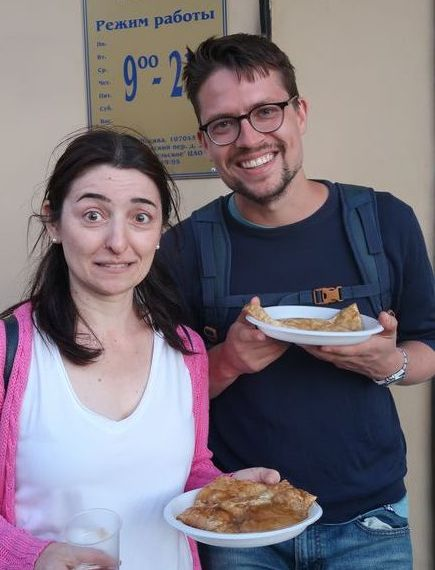
\includegraphics{images/20180603_cheburieki.JPG}
\caption{Les fameux Cheburieki, obtenus grâce à Irma.}
\end{figure}

On vous laisse avec quelques photos (dont l'une a été réalisée avec un
trucage optique, on attend vos commentaires pour savoir si ça se voit).
Prochaine étape : Saint Pétersbourg, la Venise du nord, et ses nuits
blanches.

Et petit bonus réalisé avec la caméra 360° (merci Vaness ;) ).

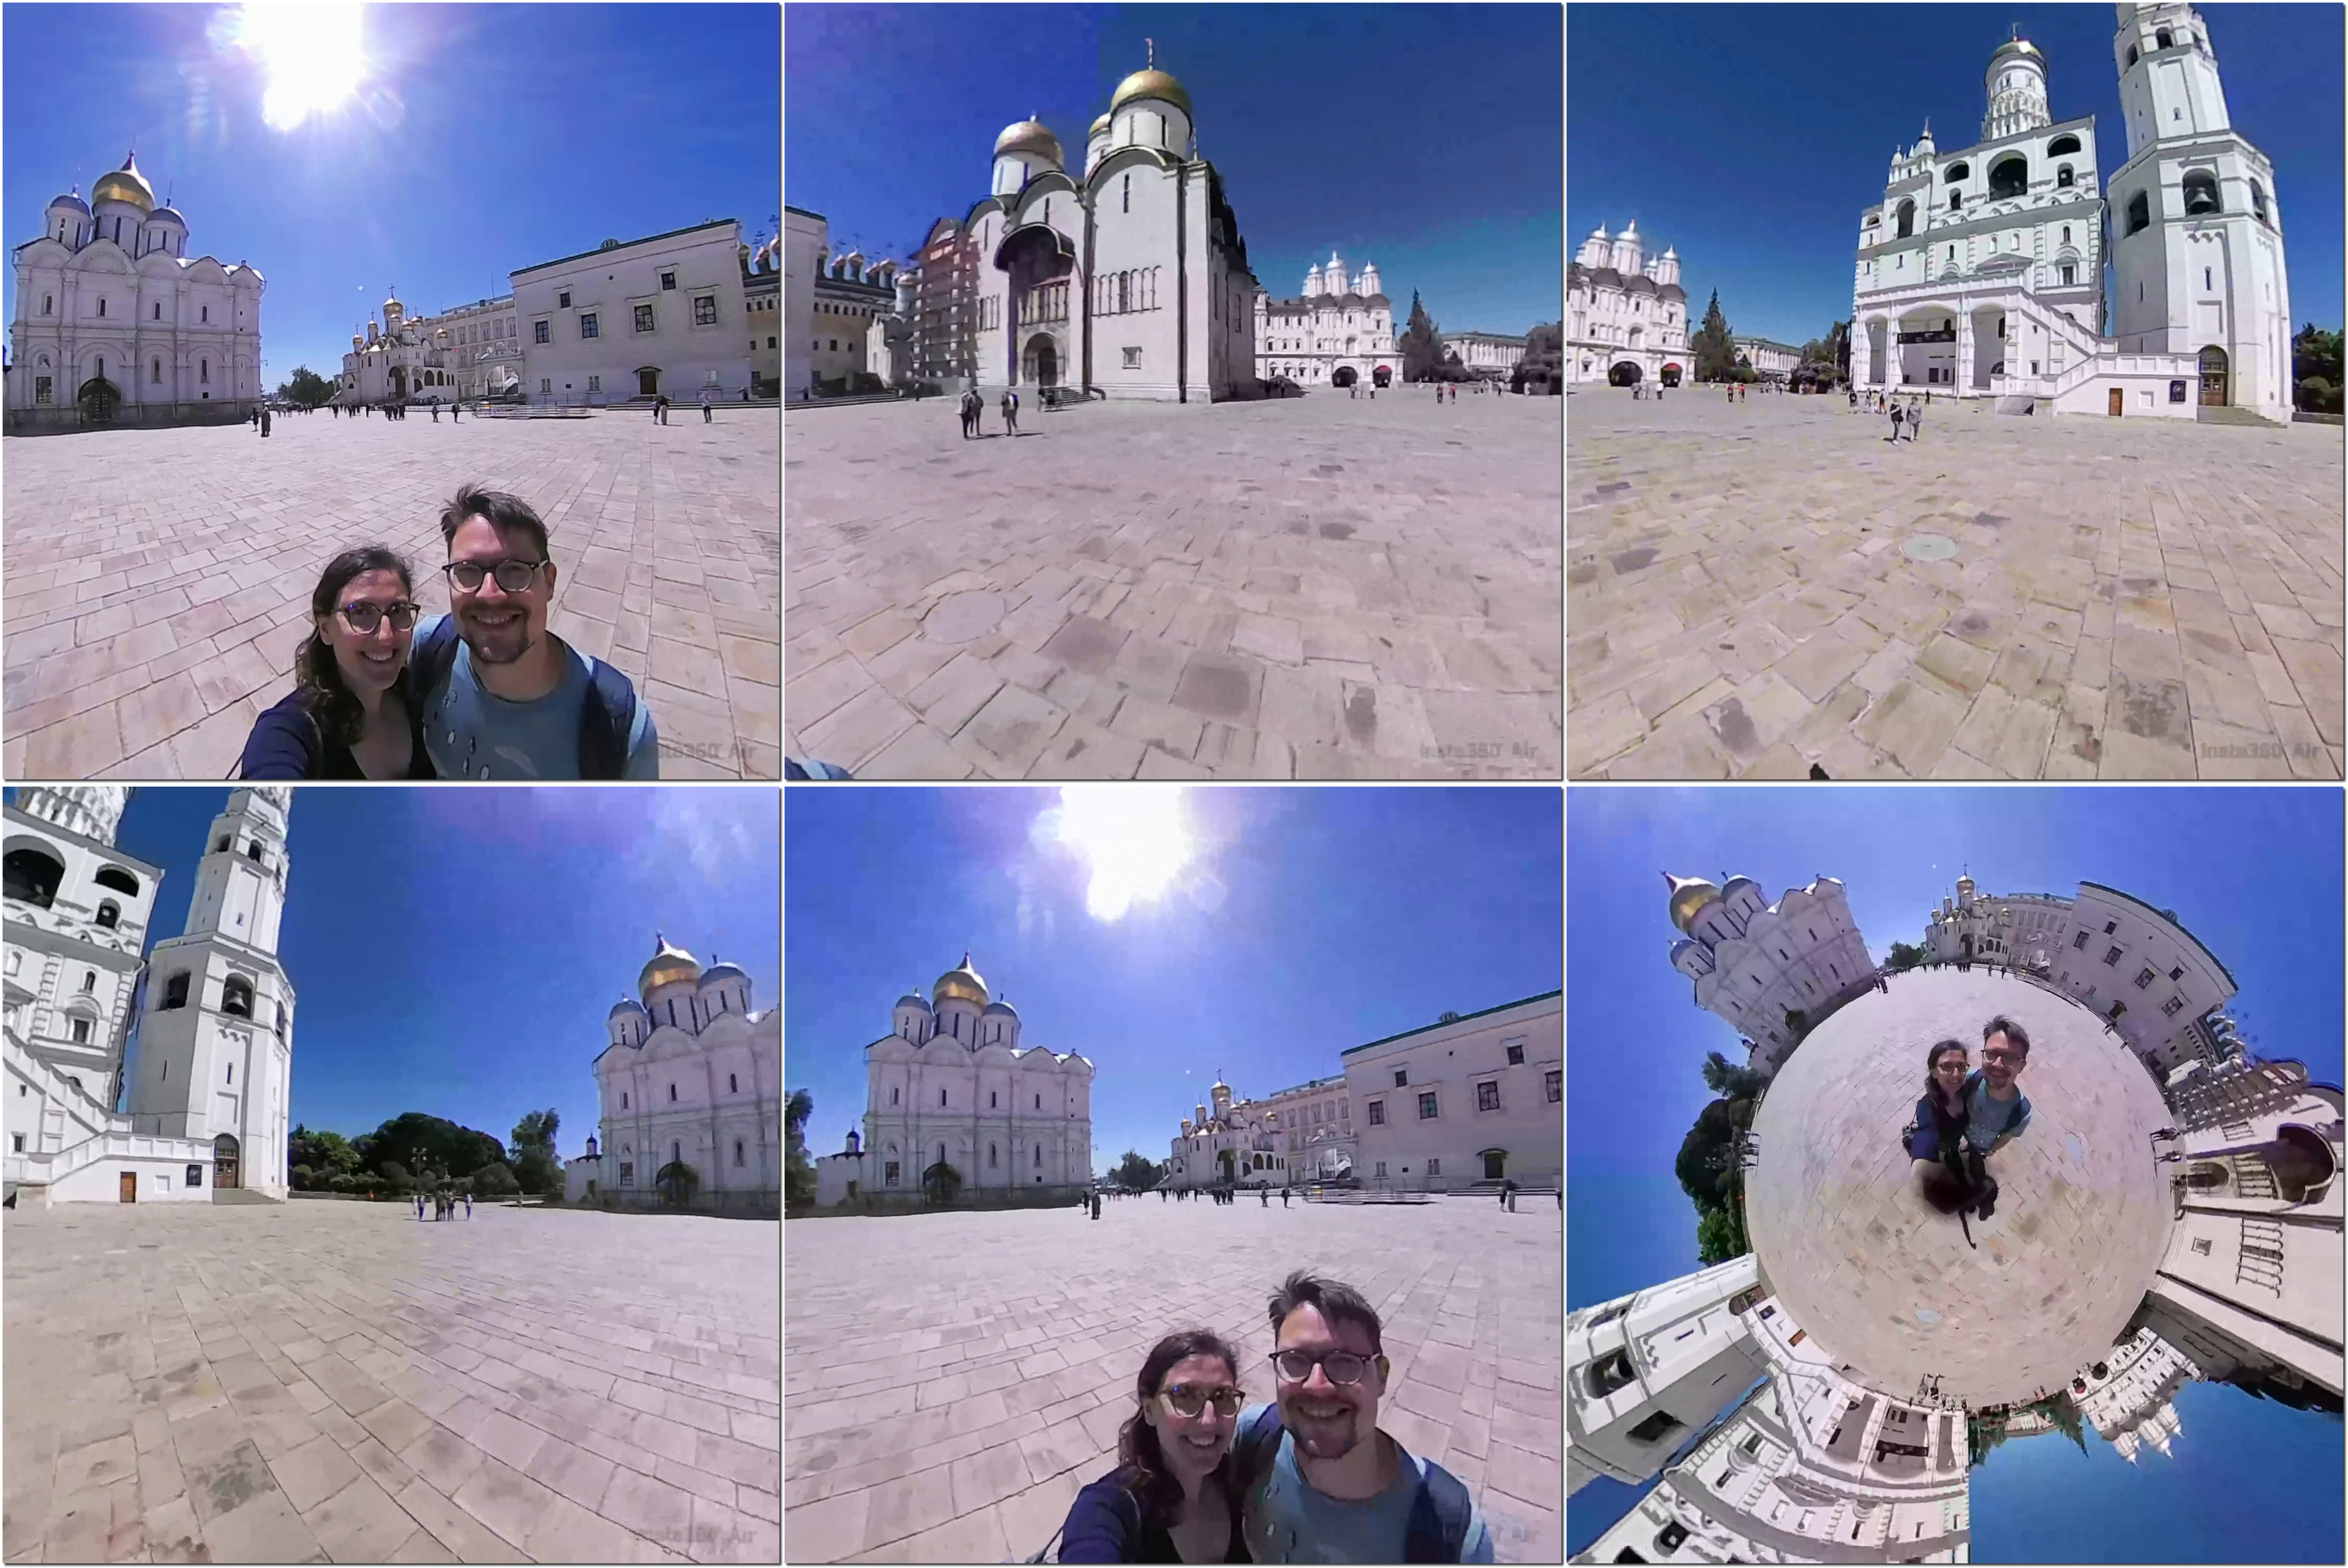
\includegraphics{montage/russie.jpg}

\emph{Elida et Florian}

\hypertarget{commentaires}{%
\subsection{Commentaires}\label{commentaires}}

\begin{itemize}
\item
  ZRC, \emph{2018-06-03 15h48}

  Moi je dis que la statue de la photo 23 ne repose pas exactement sur
  l'eau... Flo aurait pu citer un texte qu'on a vu en cours de russe,
  qui disait que la vie était dure et qu'on ne souriait pas pour rien en
  Russie.
\item
  Thibaud, \emph{2018-06-03 17h59}

  C'est vrai que la photo 23 est chelou.\\
  J'avais lu à peu près la même chose sur les sourires en Russie : on ne
  sourit pas juste par politesse, ça peut d'ailleurs être considéré
  comme offensant !
\item
  Florian LB, \emph{2018-06-03 21h04}

  Je ne savais pas tout ça. Du coup, je viens de taper la requête dans
  mon moteur de recherche favori et il semble que le sourire russe soit
  un point d'interrogation pour beaucoup de gens. Me voilà rassuré. :-)
\item
  Florian LB, \emph{2018-06-03 20h52}

  Ah zut, je ne m'en souviens pas ! Tu crois que tu peux retrouver le
  texte et le mettre ici ?

  En tout cas bravo, tu as trouvé la photo truquée ! On a utilisé un
  écran de smartphone pour donner un reflet de ciel à l'image.
\item
  Timothée Nicolas, \emph{2018-06-03 21h05}

  C'est magnifique et très intéressant ! On a hâte d'en savoir plus !
\end{itemize}


\hypertarget{saint-puxe9tersbourg-berceau-de-la-ruxe9volution}{%
\section{Saint-Pétersbourg, berceau de la
révolution}\label{saint-puxe9tersbourg-berceau-de-la-ruxe9volution}}

C'est en train que nous avons rejoint Saint-Pétersbourg depuis Moscou.
Quatre heures, c'est le temps qu'on met à relier la ville nouvelle
fondée en 1703 par Pierre le Grand depuis la capitale actuelle. Nous y
avons passé presque une semaine et, au fil des balades à pied, découvert
une ville riche en palais colorés.

Comme un écho aux lourdes pierres de Baalbeck, on y trouve cette statue
équestre de Pierre le Grand :

\begin{figure}
\centering
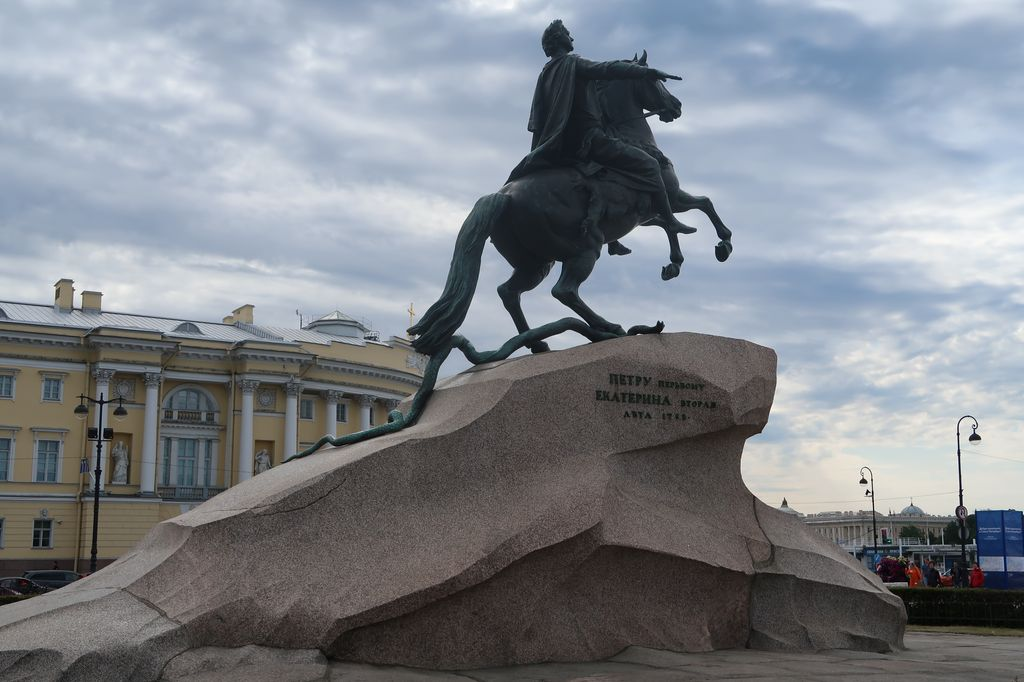
\includegraphics{images/20180606_pierre.JPG}
\caption{A notre droite, l'Ermitage, devant nous, la Neva et sous nous,
le granit.}
\end{figure}

On peut à ce sujet citer l'article de Jean-Pierre Adam justement déniché
lors de \href{/au-revoir-liban.html}{notre billet précédent}.

\begin{quote}
1.250.000 kilogrammes ! c'est le poids du formidable bloc de granite
(sic) que l'impératrice de Russie Catherine II (1762 à 1796) fit
transporter à Saint-Pétersbourg (aujourd'hui Leningrad) pour servir de
socle colossal à la statue équestre de Pierre le Grand. Il s'agit là
fort probablement de la plus grosse pierre jamais déplacée par l'homme,
une fois et demie le poids des blocs du trilithon.
\end{quote}

Mais Saint-Pétersbourg, après sa fondation comme nouvelle capitale de la
Russie des Tsars, a également été le siège de l'un des évènements les
plus marquants du XXème siècle (dixit notre ami Stanislav) : la
révolution d'octobre. Pour résumer, la prise de pouvoir des communistes
et le renversement du gouvernement provisoire après l'abdication des
Tsars en 1917 a entraîné la création de l'Union Soviétique à l'issue des
années de guerre civile qui ont suivi. Et c'est ici que cela a commencé.

\begin{figure}
\centering
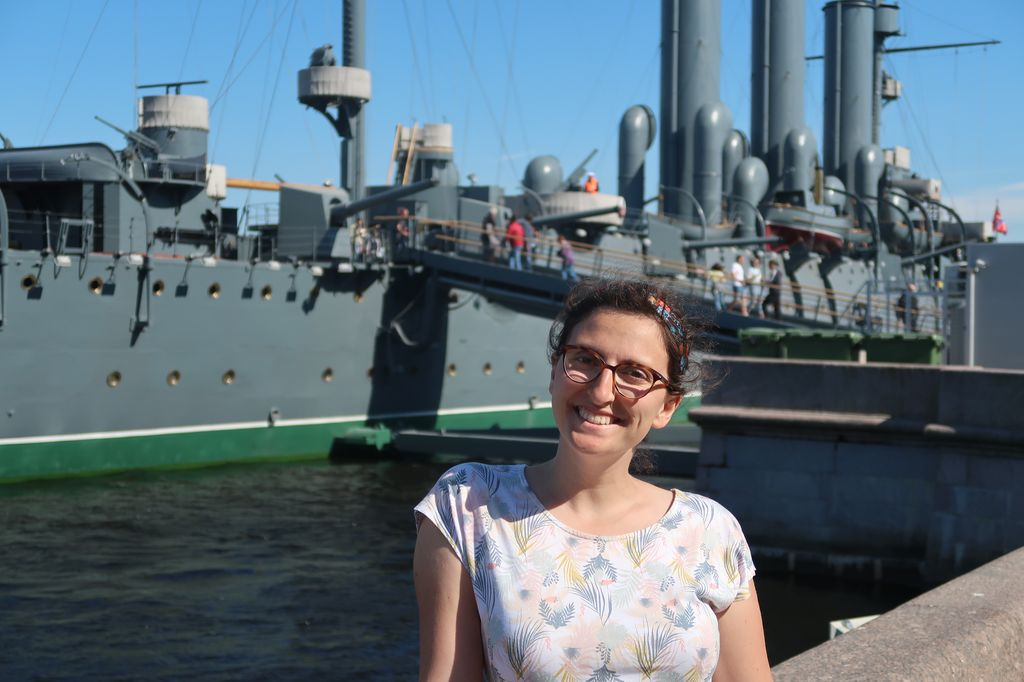
\includegraphics{images/20180606_Aurora.JPG}
\caption{Elida et le croiseur Aurora, contemporain aujourd'hui muet de
la révolution d'octobre, mais qui a donné le signal le jour J (en tirant
à blanc des coups de canon pour lancer l'assaut.}
\end{figure}

Avant de clore ce billet, il faut également mentionner que nous sommes
ici à une latitude bien plus élevée qu'à Paris. En conséquence, les
journées sont très longues et le soleil ne se couche presque pas à ce
moment de l'année. Cela rend d'autant plus agréable les nombreuses
balades par temps clair que nous avons pu faire. En particulier, nous
avons apprécié le lever des ponts de la ville, moment d'affluence
étonnant sur les berges et les eaux de la Neva à 1h30 du matin. En
principe rendu nécessaire par la navigation fluviale, c'est aussi l'une
des attractions constamment proposées aux touristes dans la ville. Mais
le charme opère, après une longue soirée à écouter un groupe de rock
russe sur la place de l'Ermitage...

\begin{figure}
\centering
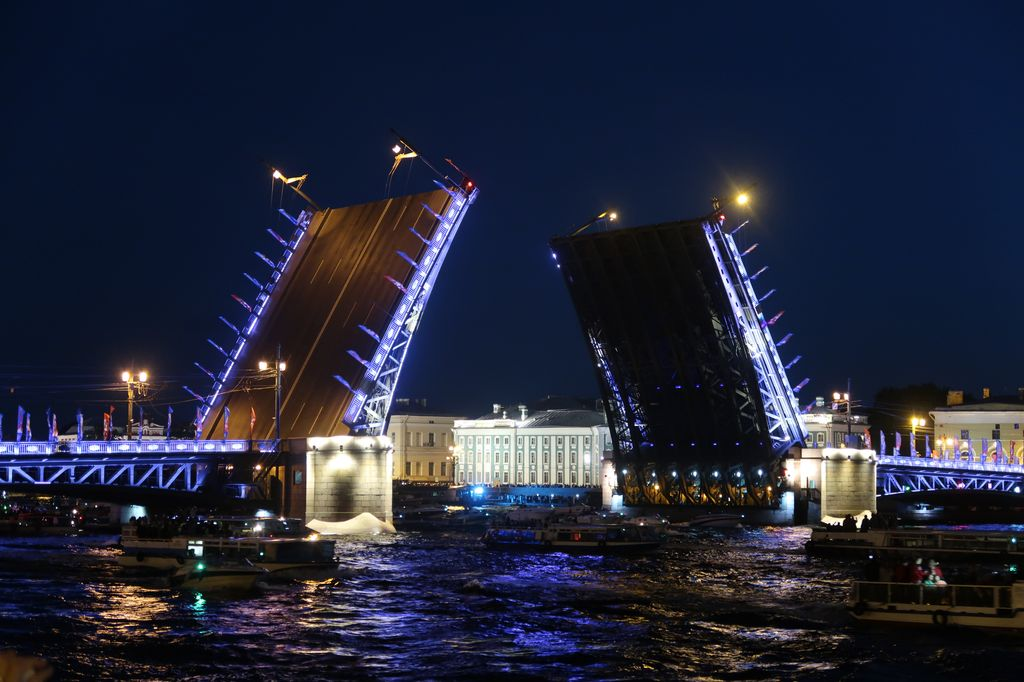
\includegraphics{images/20180606_pontpalais.JPG}
\caption{Le pont du palais vers 1h40 du matin.}
\end{figure}

Sur ce, nous vous donnons rendez-vous en Chine pour notre prochain
article !

\emph{Florian et Elida}

\hypertarget{ux434ux43e-ux441ux432ux438ux434ux430ux43dux438ux44f-russie}{%
\section{До свидания, Russie
!}\label{ux434ux43e-ux441ux432ux438ux434ux430ux43dux438ux44f-russie}}

\emph{Samedi 09 juin 2018}

Le temps file à vive allure. Et il nous amène déjà à notre prochaine
destination. Nous avons donc passé nos deux derniers jours à dire
au-revoir à nos amis russes en festoyant, tout en gardant pour la fin de
notre séjour une visite au musée Pouchkine.

\begin{figure}
\centering
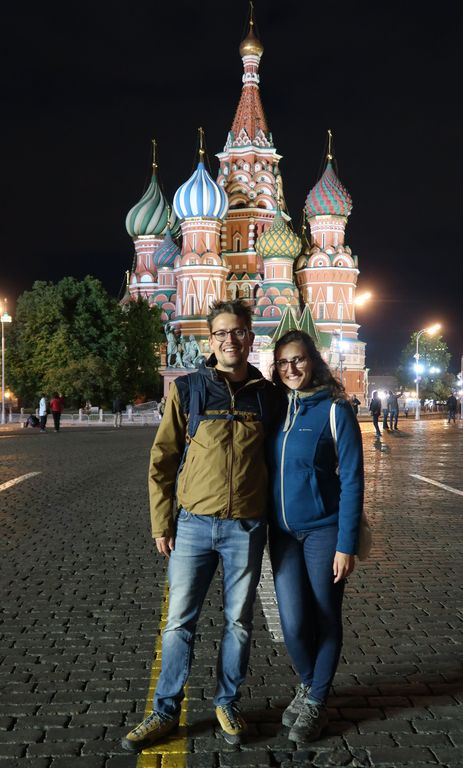
\includegraphics{images/20180609_aurevoir.JPG}
\caption{Souvenir du dernier soir : la place Rouge et la cathédrale de
Basile.}
\end{figure}

Pourquoi cette visite ? Les lecteurs attentifs de ce blog apprécieront :
inspirés par
\href{https://www.franceinter.fr/emissions/sur-les-epaules-de-darwin/sur-les-epaules-de-darwin-10-mars-2018}{une
récente émission de Jean-Claude Ameisen}, nous sommes allés voir le
"trésor de Priam" découvert lors des fouilles sur la côte turque par
Heinrich Schliemann à la fin du XIXème siècle. Cédé à un musée berlinois
par l'archéologue, le trésor avait disparu lors de la prise de
l'Allemagne en 1945 par l'union soviétique. Et comme l'histoire a
souvent plus d'un tour dans son sac, ce trésor est réapparu dans les
années 90 à Moscou. Cette anecodote racontée lors de l'émission était
trop belle pour rater cette visite. D'autant plus que le musée présente
également de belles tablettes mésopotamiennes...

Avant de nous diriger vers l'aéroport qui va nous emmener en Russie,
nous faisons le tour des stations de métro sur la ligne circulaire de
Moscou et admirons une dernière fois la diversité et la qualité de cet
endroit. Direction : la Chine !

\emph{Florian et Elida}

\hypertarget{arrivuxe9e-dans-lempire-du-milieu}{%
\section{Arrivée dans l'empire du
milieu}\label{arrivuxe9e-dans-lempire-du-milieu}}

\emph{Lundi 11 juin 2018}

C'est au terme d'une correspondance ratée (mais reroutée avec brio par
China Southern Airlines, au prix d'une course à travers tout l'aéroport
de Wuhan) que nous sommes arrivés à Shanghai.

Nous y avons eu le plaisir de passer deux soirées avec Longhui et Chen
qui, en tant que bons connaisseurs de la France, nous ont expliqué
quelques fondamentaux sur la Chine.

\begin{figure}
\centering
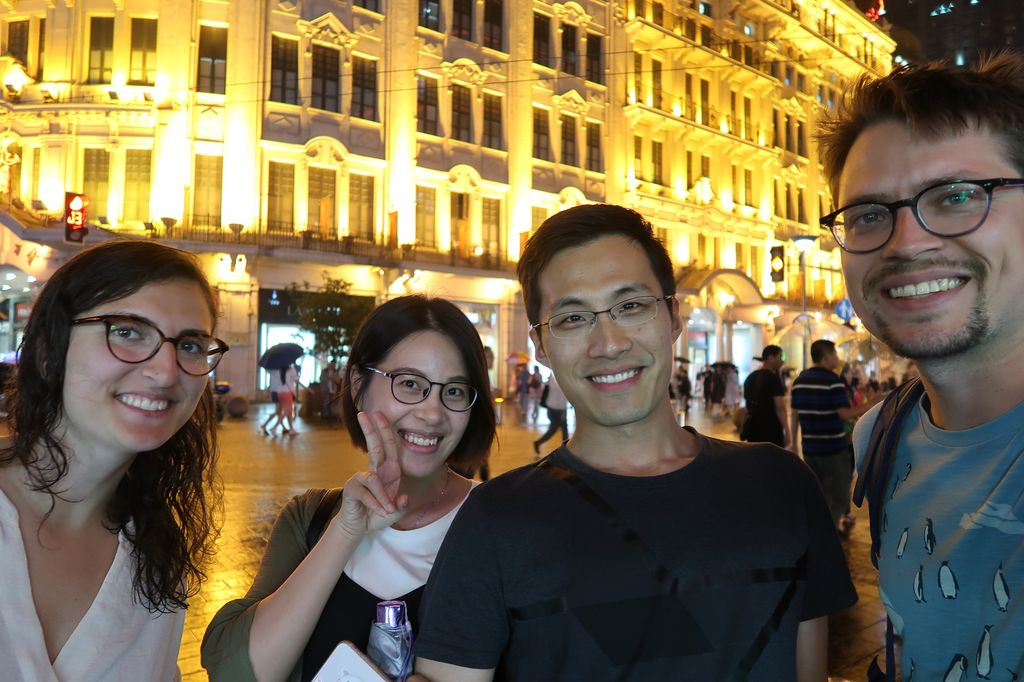
\includegraphics{images/20180611_shanghai.JPG}
\caption{Selfie 'classique' dans la rue piétonne Nanjing Road, près du
Bund.}
\end{figure}

Nous avons ensuite admiré la vue depuis la promenade du Bund, sur les
berges du fleuve Huangpu.

\begin{figure}
\centering
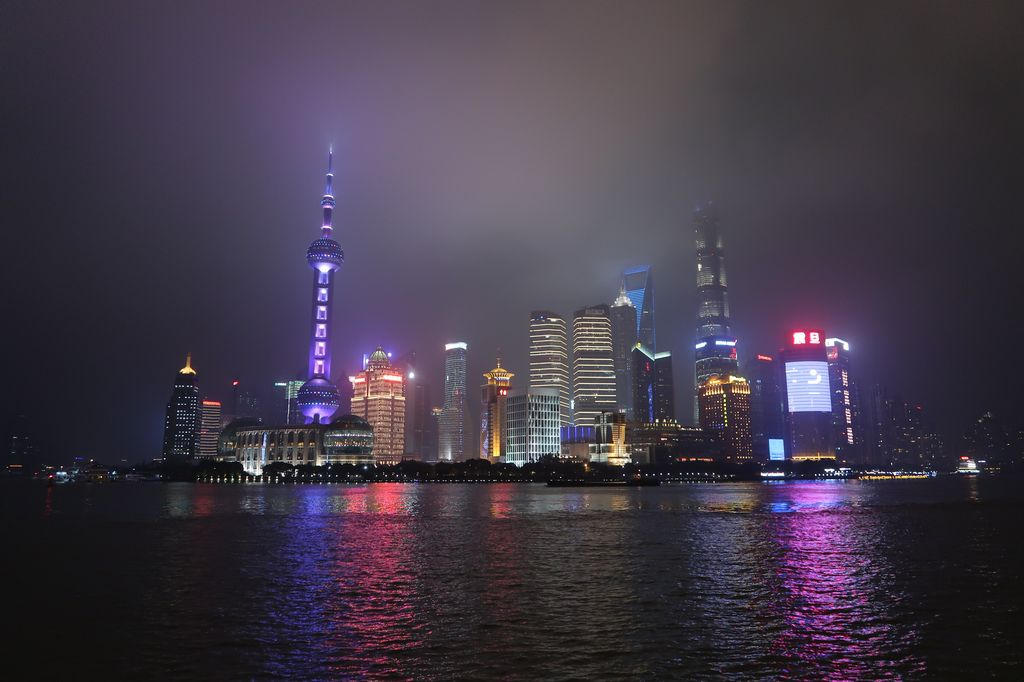
\includegraphics{images/20180611_bund.JPG}
\caption{La vue sur les gratte-ciels de la nouvelle ville de Shanghai,
Pudong.}
\end{figure}

Tout ceci augure de belles découvertes pour notre tour de la Chine dans
les deux prochaines semaines !

\emph{Florian et Elida}

\hypertarget{la-chine-au-pas-de-course}{%
\section{La Chine au pas de course}\label{la-chine-au-pas-de-course}}

\emph{Samedi 16 juin 2018}

Depuis notre arrivée en Chine, le rythme de notre voyage s'est accéléré.
Après avoir passé deux semaines pour visiter deux villes en Russie, la
cadence de deux jours par ville est un peu rude ! Les étapes de notre
parcours jusqu'ici ont été : Shanghai, Suzhou, Beijing, Gubeikou, Xi'an.

Après nos deux premières nuits à Shanghaï, marquées surtout par une très
mauvaise tolérance du décalage horaire surajouté à la nuit blanche du
voyage (on vous a pas raconté la correspondance ratée, mais elle a été
marquée par une scène mythique de course à travers l'aéroport de Wuhan
avec nos sac à dos, derrière l'employé de la compagnie qui arrêtait pas
de crier "hurry up! hurry up!", alors que bon les 3 heures de retard de
notre vol, on les avait pas vraiment demandées...), on a pris un train
pour notre première étape : Suzhou.

Première expérience de train, un peu effrayante (surtout qu'on venait
d'acheter pour 200 euros de billets de train à travers le pays) : ce
sont des trains type TER, donc pas très rapides et faisant de nombreux
arrêts, d'allure plutôt vétuste. Il y a 5 sièges par rangée, face à
face, dont l'assise fait à peine plus que la moitié des assises
auxquelles ont est habitués. Les tout petits porte-bagages sont pris
d'assaut par les sacs de courses des gens qui rentrent en banlieue
(c'est pas l'Essonne hein, on parle d'un tout autre ordre de
grandeur...) et le train est complètement surbooké, avec des gens debout
dans tous les sens. Les contrôleurs jouent à se chamailler entre eux,
les gens se pressent au distributeur d'eau chaude pour manger leur boite
de nouilles instantanées ou juste remplir leur gourde à thé qu'ils ne
lâchent pas. Bon, on va dire que pour une heure de train, ça se fait
plutôt bien, et puis c'est un peu une "expérience d'un autre âge" (clin
d'oeil à Ruocong).

\begin{figure}
\centering
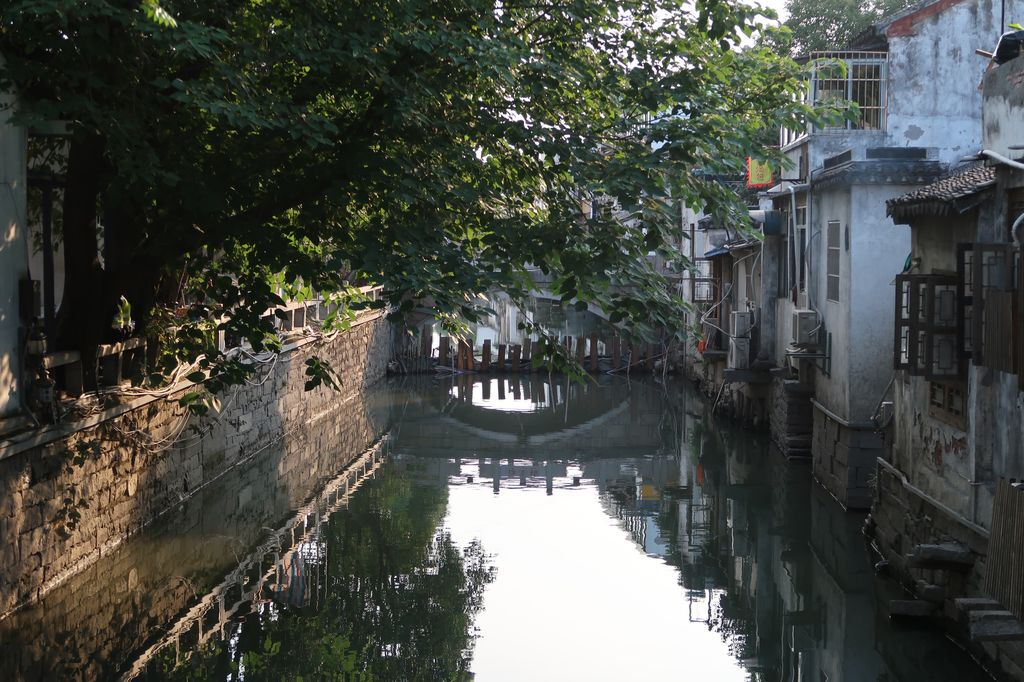
\includegraphics{images/20180616_suzhou.JPG}
\caption{L'un des canaux du vieux centre de Suzhou.}
\end{figure}

Faut dire qu'après ça, on était bien contents de prendre un taxi pour
rejoindre notre auberge, sur le canal central de la ville. Oui parce que
Suzhou, c'est "la Venise de l'Orient", une ville dont le centre est
quadrillé par des canaux et ponctuée par des jardins traditionnels aux
noms rigolos dispersés à ses quatre coins. Les balades au fil de l'eau
étaient plutôt agréables, mais l'agrément des jardins était vite altéré
par les hordes de touristes à perche (à selfie). Le meilleur moment de
notre court séjour a été la visite d'un temple bouddhiste, un peu à
l'écart. On a été accueillis par une statue de Bouddha souriant devant
une belle pagode, mais aussi par une dame qui travaille dans le temple
et qui a appris à Elida à prier en chinois, puis par un maître
calligraphe qui nous a appris à écrire "France" sur le sol du temple,
puis par un moine bouddhiste qui nous a offert des délicieux fruits dont
on n'a toujours pas réussi à retenir le nom, puis par un monsieur de
Pékin qui se prélassait sur un promontoire et qui a discuté avec nous
pendant que nous sortions ensemble du temple. Un vrai moment de calme et
de générosité...

Mais le calme est de courte durée, nous avons un train de nuit à
attraper pour notre troisième étape : Pékin !

Deuxième expérience de train, que nous abordons avec méfiance, surtout
qu'il s'agit de rester 11 heures dans le machin. C'est finalement une
très agréable surprise, car les trains de la ligne Shanghaï-Pékin ont
été récemment remplacés par des trains-couchette extrêmement
confortables et bien équipés. D'après Flo, grand habitué des voyages
nocturnes : "c'est le meilleur train de nuit de toute ma vie !", et on
était qu'en deuxième classe !

\begin{figure}
\centering
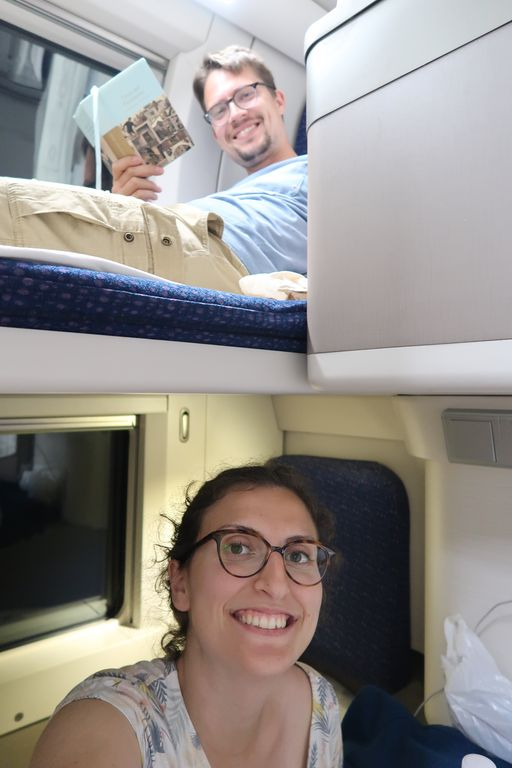
\includegraphics{images/20180616_trainnuit.JPG}
\caption{Selfie dans le train de nuit D312. Flo est en train de lire
Dostoïevski, souvenir emporté de Russie.}
\end{figure}

Nos premiers pas à Pékin nous propulsent un peu plus loin dans le
dépaysement. Notre auberge, le Red Lantern (coucou les Thibali ! on a vu
\emph{a posteriori} que vous y êtes passés aussi !) se trouve dans un
\emph{hutong}, un de ces quartiers typiques de la ville constitués de
ruelles et de petites maisons basses. Et comme on est levés tôt, on
commence la journée par la visite de la Cité Interdite ! Cet
enchaînement de palais en enfilade qui se termine par un jardin nous
fait voyager plus de 500 ans en arrière... et le flot dense de touristes
nous ramène à la réalité, et rend la visite vite pénible (80 000
touristes par jour, c'est 1 fois et demi Disneyland Paris en plein été).
Voilà que l'orage s'en mêle et on s'abrite dans les petits palais
latéraux où sont exposés des objets des différentes dynasties. Le temps
que la météo se calme, on est devenus experts en céramique chinoise ;)
On continue la journée par une balade depuis les "Drum Tower" et "Bell
Tower", anciennes tours jumelles qu'on retrouvera en fait dans toutes
les vieilles villes du pays, puis par le parc Beihai et le parc Jingshan
depuis lequel on a une vue panoramique sur la Cité Interdite et sur un
beau coucher de soleil sur Pékin.

\begin{figure}
\centering
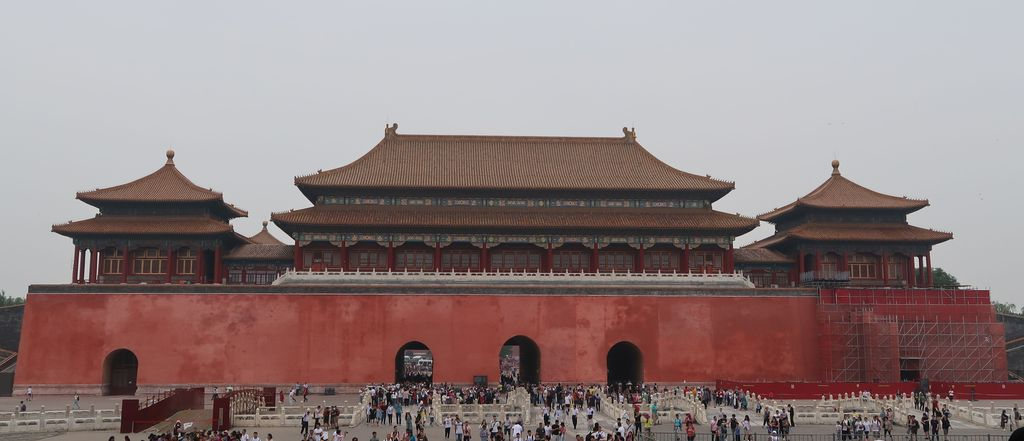
\includegraphics{images/20180616_cite.JPG}
\caption{L'un des palais de l'Harmonie de la Cité Interdite}
\end{figure}

La visite du Palais d'Eté le lendemain nous permettra de nous échapper
de la chaleur étouffante de la ville. On se s'attarde pas sur les
bâtiments, mais la visite est tout de même intéressante. Le tour du lac
nous permet de nous écarter des foules, ce qui est toujours très
agréable ! Le soir, sur des recommandations expertes, nos papilles
découvrent le vrai canard à la pékinoise, grillé à point et découpé avec
art sous nos yeux. Nous qui étions soucieux de ne pas pouvoir finir un
canard entier, nous l'avons dévoré jusqu'à la dernière miette !

\begin{figure}
\centering
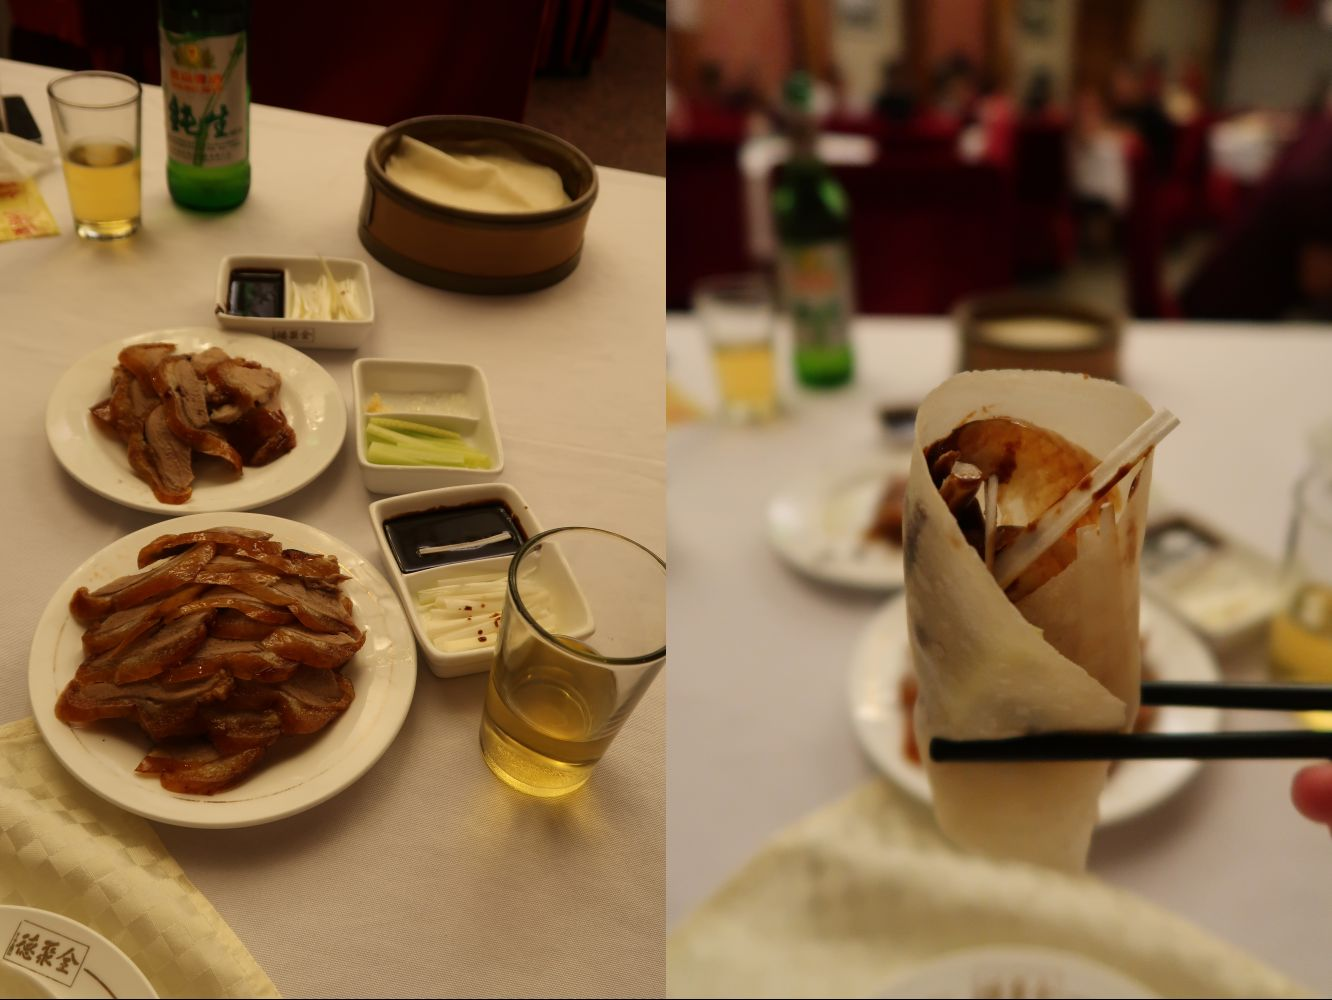
\includegraphics{images/20180616_canard.jpg}
\caption{Avant / après : voici comment on nous a appris à manger le
canard de Pékin.}
\end{figure}

Nous avons fait nos derniers pas à Pékin au temple des Lamas, constitué
de plusieurs bâtiments successifs dont la magnificence va crescendo
jusqu'au dernier où trône une statue de Bouddha debout de 18 mètres de
haut taillé dans une seule pièce de bois. Après avoir avalé un délicieux
Jianbing (une sorte de crêpe salée à l'oeuf et au sésame, garnie de
salade, d'oignon vert, de sauces diverses et de tofu grillé), on part
pour un périple en bus qui nous prendra 4 heures pour une destination
reculée : Gubeikou.

A Gubeikou nous attend Angela, notre hôte, avec un délicieux repas à
base de légumes de son potager, mais surtout la grande muraille de Chine
! Quelques dizaines de minutes de marche et la muraille est sous nos
pieds, d'aspect brut, sans rénovation. Il semble incroyable qu'on ait pu
construire un tel édifice... Comme on a fait l'effort de se lever tôt,
on passe près de 2 heures complètement seuls sur la muraille, entourés
de nombreux oiseaux, dans l'air frais du matin. L'expérience est unique,
la muraille s'étend à perte de vue des deux côtés au milieu d'une forêt
luxuriante, et même sur le flanc raide d'une montagne au loin.

\begin{figure}
\centering
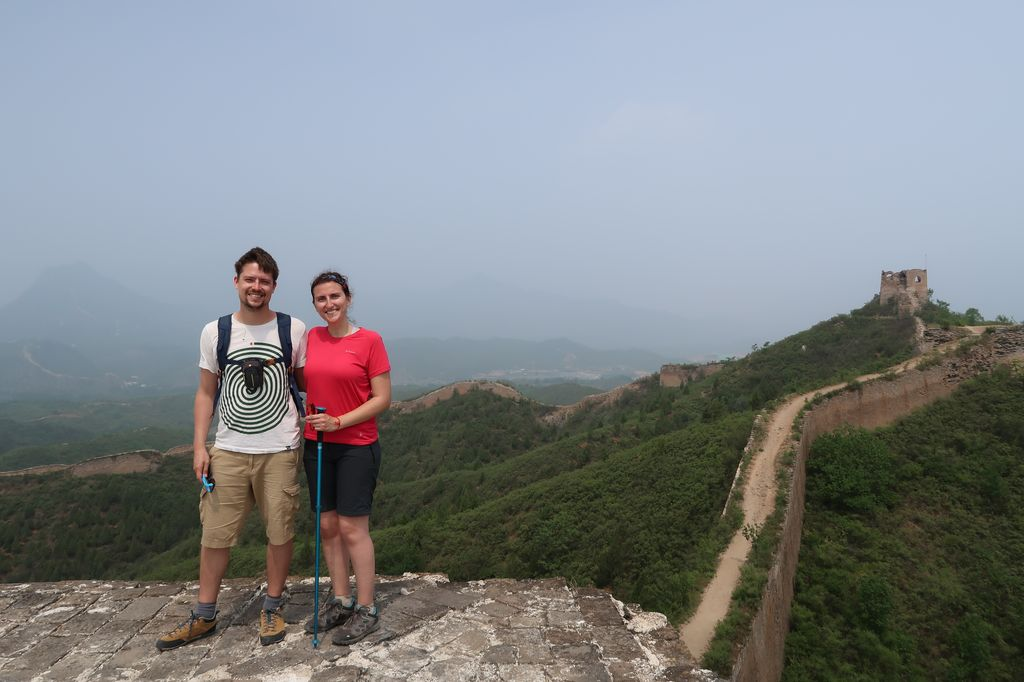
\includegraphics{images/20180616_muraille.JPG}
\caption{Debout sur la muraille de Chine, un moment dont on se
souviendra longtemps.}
\end{figure}

C'est avec un petit pincement au coeur qu'on quitte ce coin de
tranquilité pour notre deuxième train de nuit, direction Xi'an. Mais ça,
c'est pour la prochaine fois !

\emph{Elida et Florian}

\hypertarget{deuxiuxe8me-semaine-et-impressions-uxe0-lencre-de-chine}{%
\section{Deuxième semaine et impressions (à l'encre) de
Chine}\label{deuxiuxe8me-semaine-et-impressions-uxe0-lencre-de-chine}}

\emph{Vendredi 22 juin 2018}

Notre deuxième semaine en Chine a continué au même rythme que la
première. Nous en ressortons donc fatigués après avoir exploré les
villes de Xian, Luoyang et Nanjing.

\hypertarget{les-derniuxe8res-uxe9tapes}{%
\subsection{Les dernières étapes}\label{les-derniuxe8res-uxe9tapes}}

\begin{figure}
\centering
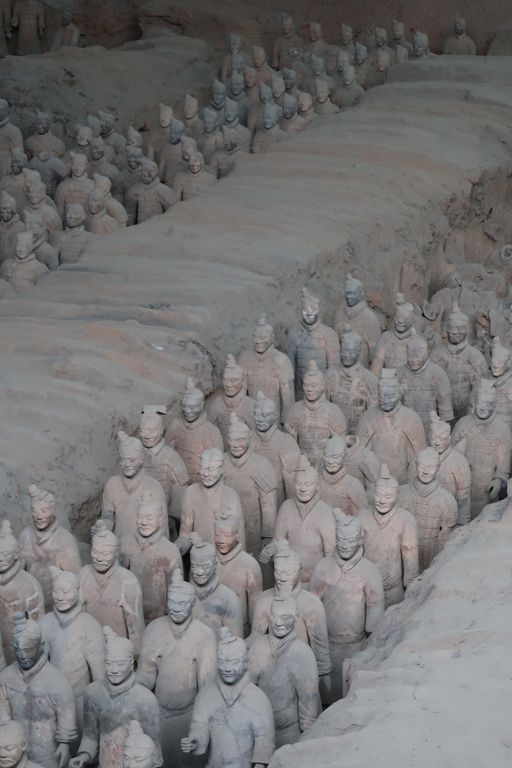
\includegraphics{images/20180622_terracotta.JPG}
\caption{Les soldats de terre cuite, rangés en ordre de bataille pour
l'au-delà.}
\end{figure}

A Xian, nous avons visité le parc des soldats de terre-cuite de
l'empereur Qin. Premier unificateur de la Chine, fervent croyant dans la
vie après la mort, il semblerait qu'il ait voulu poursuivre ses
conquêtes dans l'au-delà à l'aide d'une armée de statues de soldats, de
cavaliers, d'archers et même de généraux. Ce parc est en fait une
fouille archéologique qui continue d'évoluer depuis la découverte des
statues en 1974 (après deux millénaires passés sous terre et oubliées du
monde). Ce qui impressionne est d'abord le nombre de statues, mais aussi
le fait que chacune soit différente, avec un visage unique. L'armée est
bien fournie, avec des généraux, des chars, des cavaliers, des archers
et des fantassins. Et quand on imagine que chacune était peinte, ce
devait être incroyable ! L'affluence est tout simplement énorme. Pour
l'anecdote, le record est à 460 000 visiteurs en un jour (soit dix fois
Disneyland en régime de pointe, pour une surface visitable bien
moindre). On est à peine surpris que le sol du pavillon d'exposition est
glissant à cause de l'humidité apportée par les hordes de touristes.

A Xian, nous avons également été surpris de voir de nombreux chinois
danser dans les rues (des sortes de milongas de danse traditionnelle
chinoise), chose que nous avons revue à Luoyang. Par ailleurs, la ville
est agréable à parcourir à pied. Nous aurions aimé marcher sur ses
immenses remparts restaurés mais nous n'en avons pas eu le temps.

\begin{figure}
\centering
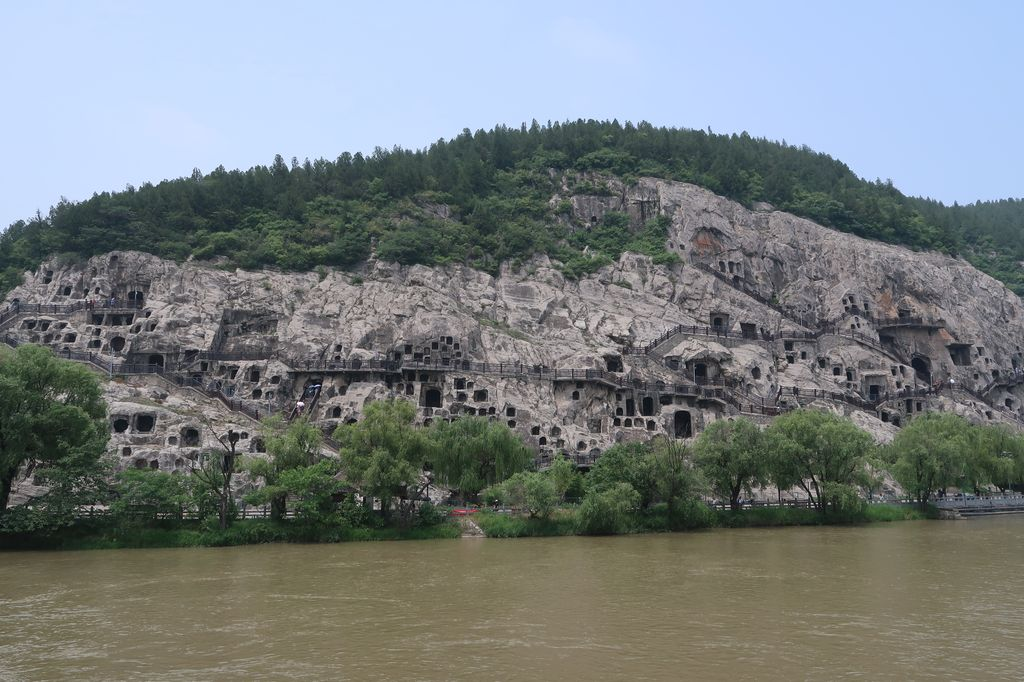
\includegraphics{images/20180622_luoyang.JPG}
\caption{Les grottes de Longmen à Luoyang. Chaque petite (ou grande)
alcôve rocheuse a accueilli une sculpture bouddhiste. Malheureusement,
la plupart a été pillée.}
\end{figure}

A Luoyang, nous avons pu explorer le très grand complexe des grottes
bouddhistes de Longmen. Des dizaines voire des centaines de milliers
d'ouvrier ont ici taillé la roche durant plusieurs centaines d'années
pour honorer la religion boudhiste.

Nous avons également visité le musée de Luoyang dans lequel nous avons
appris que la ville est célèbre pour ses pivoines (prévoir de venir au
printemps pour les admirer) depuis de nombreux siècles. Elle a également
été un point de passage important lors du commerce par la route de la
soie.

\begin{figure}
\centering
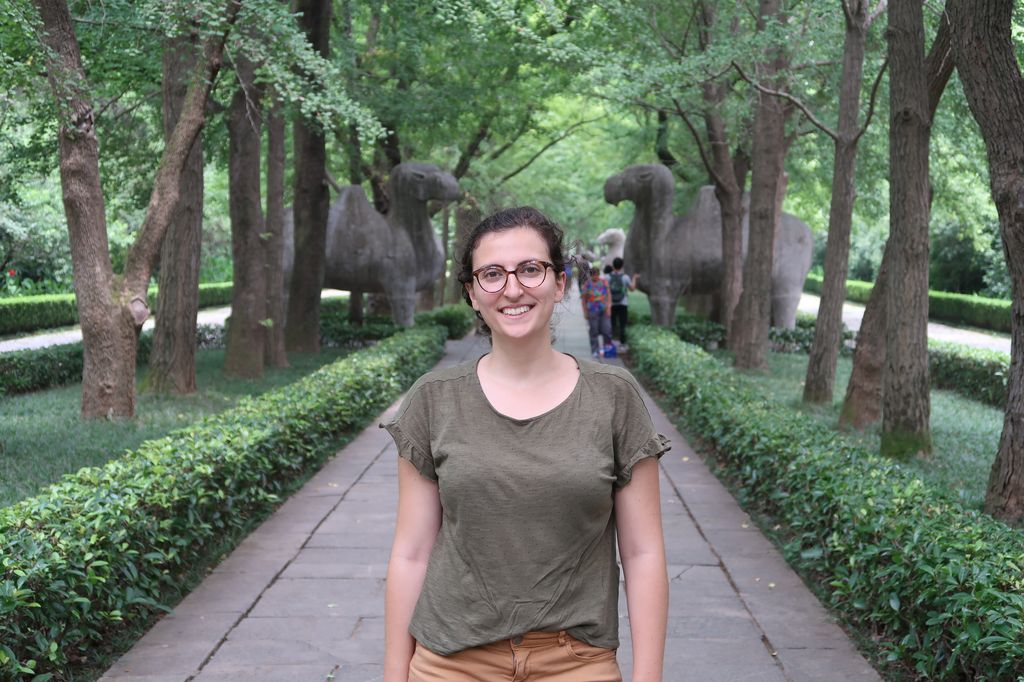
\includegraphics{images/20180622_nanjing.JPG}
\caption{Portrait dans l'allée des animaux sacrés devant la tombe Ming
de Nanjing.}
\end{figure}

Enfin, nous avons achevé de faire notre tourisme en Chine en visitant
Nanjing. On y trouve notamment, au pied de la montagne pourpre, un
sanctuaire d'un empereur de la dynastie Ming et le mémorial de Sun Yat
Sen (\emph{le} révolutionnaire chinois). Avant de quitter la ville, nous
avons visité le musée-mémorial du massacre de Nanjing, tristement
célèbre.

Voici la carte des villes que nous avons visitées lors de ces deux
dernières semaines :

\begin{figure}
\centering
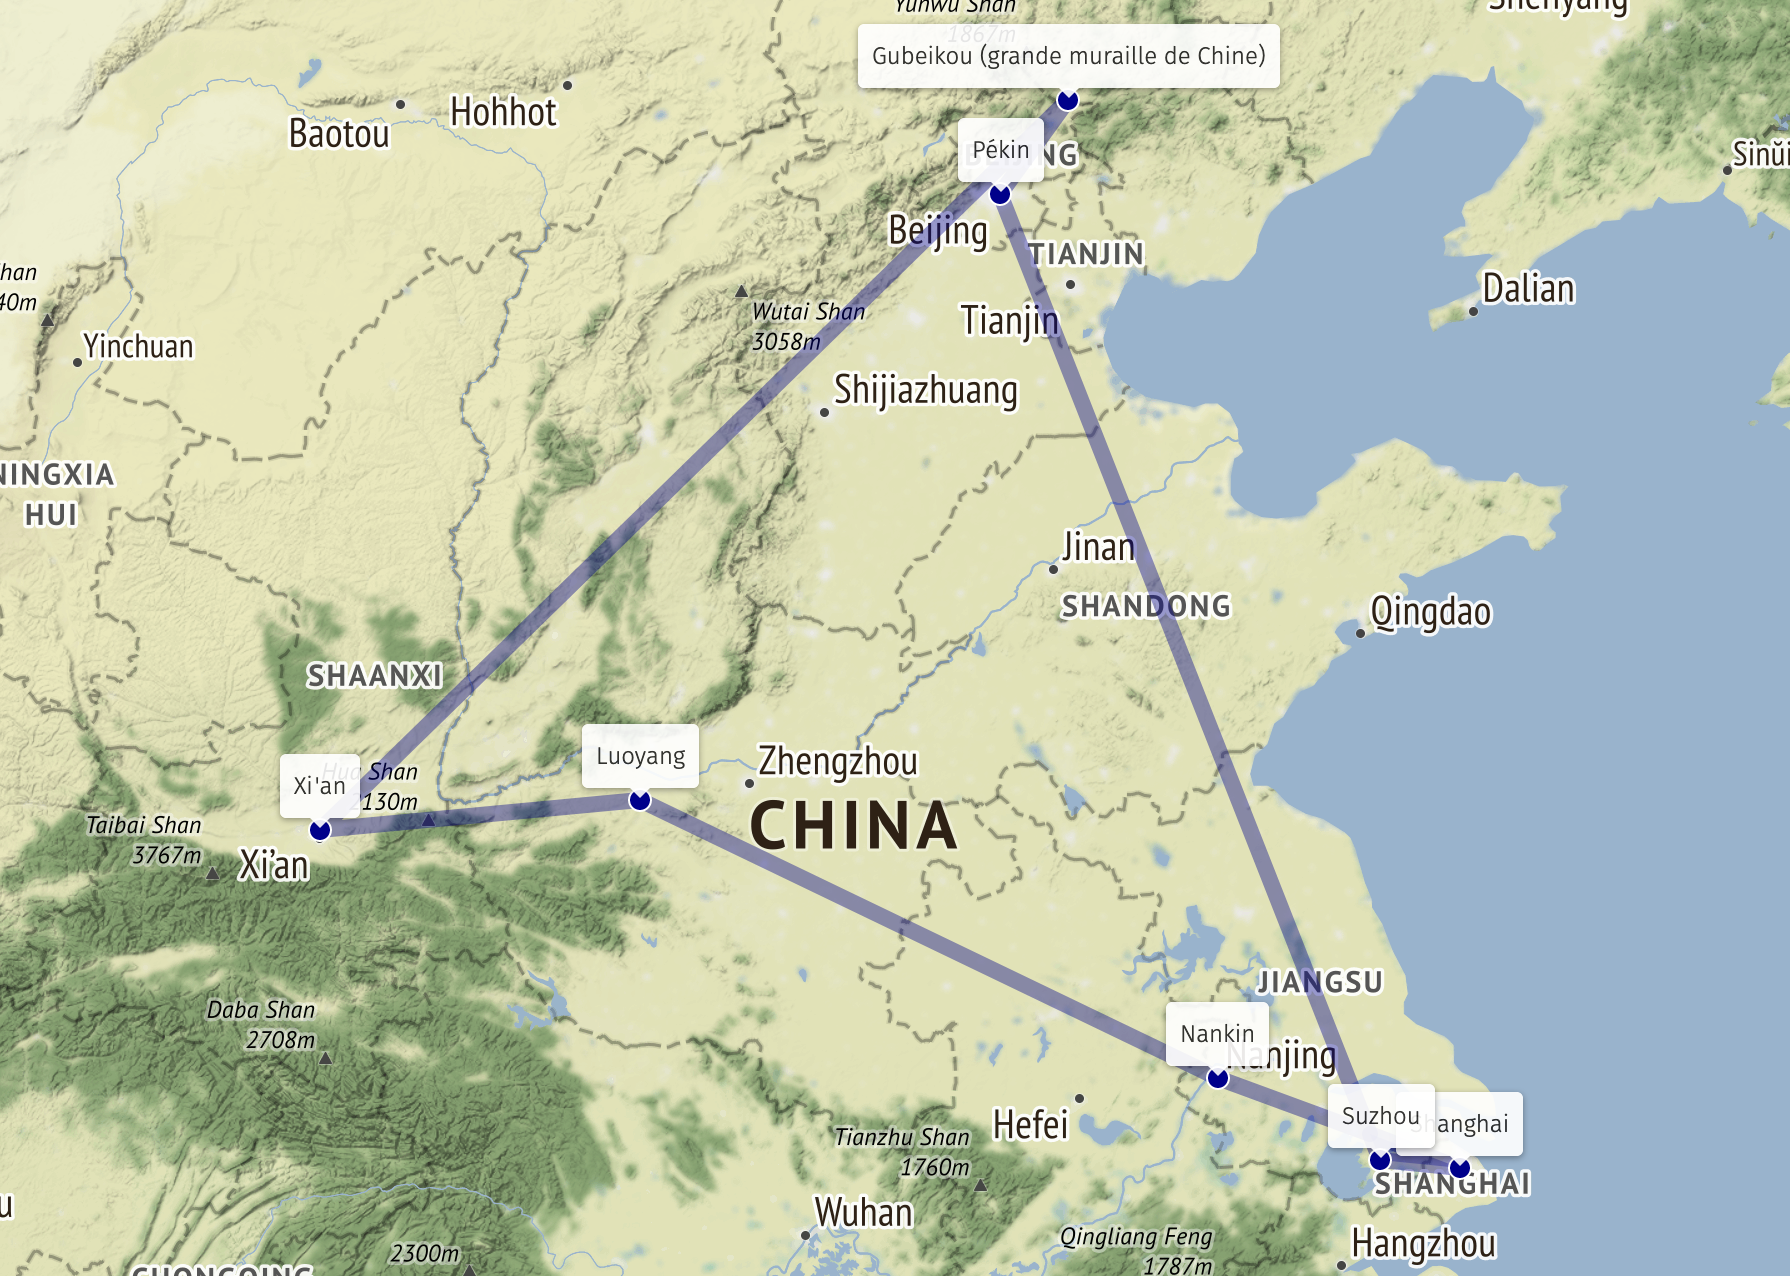
\includegraphics{maps/Chine.png}
\end{figure}

\hypertarget{et-nos-impressions}{%
\subsection{Et nos impressions ?}\label{et-nos-impressions}}

Mais avant de quitter ce beau pays qu'est la Chine, voici quelques
observations accumulées durant les deux dernières semaines.

Et autant le dire tout de suite, nous avons été fortement impressionnés
par les choses que nous avons observées. La Chine est un pays démesuré.
Les problèmes de logistique que résolvent les villes et les
infrastructures chinoises sont plusieurs ordres de grandeur au-dessus de
ce qu'on a l'habitude de voir en région parisienne. Les transports en
sont un exemple flagrant : le nombre de lignes de métro à Beijing, la
capacité des trains, la fréquence des passages, la manière d'organiser
les trajets de foules (à l'aide de barrières métalliques), la taille des
gares ferroviaires où on a des salles d'attentes dédiées par train (et
non pas une pour tous les trains)...

\begin{figure}
\centering
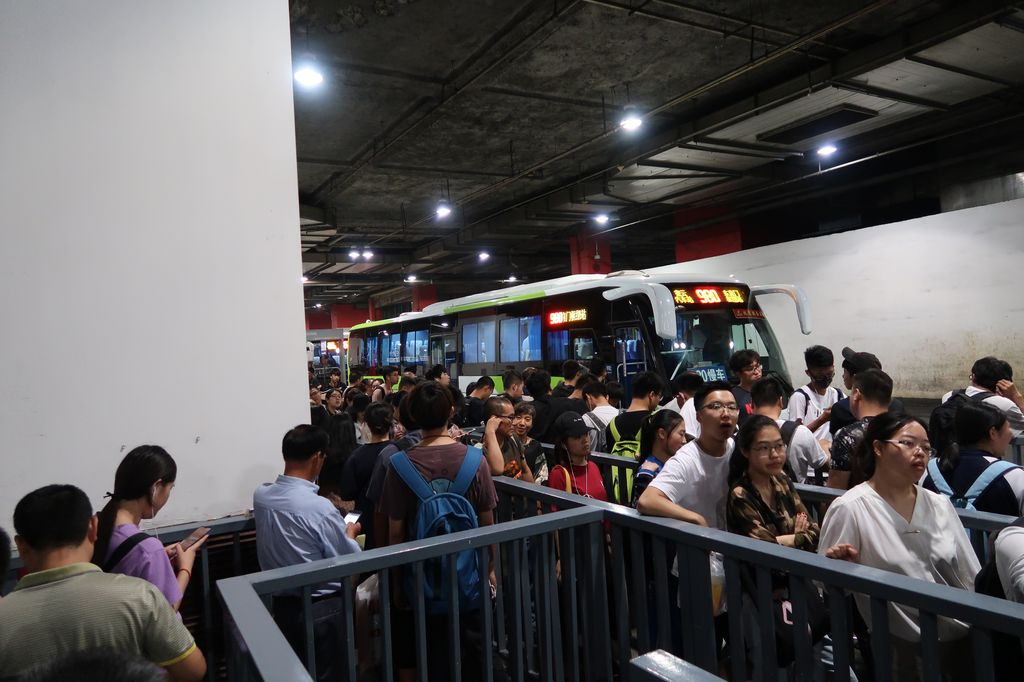
\includegraphics{images/20180622_bus.JPG}
\caption{Exemple illustratif : comment faire prendre la même ligne de
bus à 200 personnes ? 1. mettre des barrières métalliques pour guider
les gens 2. faire partir des bus toutes les cinq minutes !}
\end{figure}

Mais parlons des Chinois, que nous avons pris soin d'étudier.

Nous avons été étonnés de les voir cracher par terre (un peu partout),
fumer dans les lieux publics alors que c'est interdit, jouer des coudes
dans les transports ou dans les lieux touristiques, se tasser comme des
dingues dans le métro aux heures de pointes (à côté de ça, le RER B un
jour de grève à 8 heures du matin, c'est bon enfant), mener des
conversations téléphoniques en haut-parleur dans les transports publics.
On les croise quasiment toujours avec un thermos d'eau chaude ou de thé
à la main.En France on croise souvent des jeunes qui se baladent avec de
la musique à fond dans la rue, en Chine ce sont les personnes âgées qui
font ça, surtout dans les parcs (bon du coup c'est pas vraiment du rap
qu'ils écoutent !). On a souvent été pris en photo, parfois seulement
avec notre accord (par des adolescentes surexcitées principalement),
mais parfois plus "discrètement", si tant est que le flash à 2 mètres de
nous en pleine nuit est discret ! Même si le premier contact nous a
souvent semblé un peu froid et distant, une fois la glace brisée on a pu
échanger avec des personnes adorables et bienveillantes (un monsieur
assis à côté de nous dans le train a décidé que la barrière de la langue
ne l'empêcherait pas de nous questionner sur la France et de nous parler
de médecine traditionnelle chinoise, ce qu'il a plus ou moins réussi à
faire en jonglant avec les fonctionnalités de nos 3 téléphones
portables).

Nous avons découvert que leur nouveau Dieu s'appelle WeChat (une
application mobile un peu comme WhatsApp), qui permet de faire ses
achats en scannant le QR code du vendeur, d'afficher sa vie (comme
Facebook), de parler à ses grand-parents, de prendre le métro, de faire
des transferts d'argent, de payer le bus, d'acheter ses billets de
train, de contacter des entreprises... L'empire du milieu sous l'emprise
du smartphone ? D'après ce que nous avons vu, les transactions se font
quasiment toutes par WeChat. Lors d'une rencontre, une jeune fille nous
a même confié que ça faisait plus de six mois qu'elle n'avait pas
utilisé de l'argent papier. Si cette technologie de paiement se répand
dans le monde entier, il y a de fortes chances que les Visa et
Mastercard du futur se prénomment un jour WeChat Pay et Alipay !

\begin{figure}
\centering
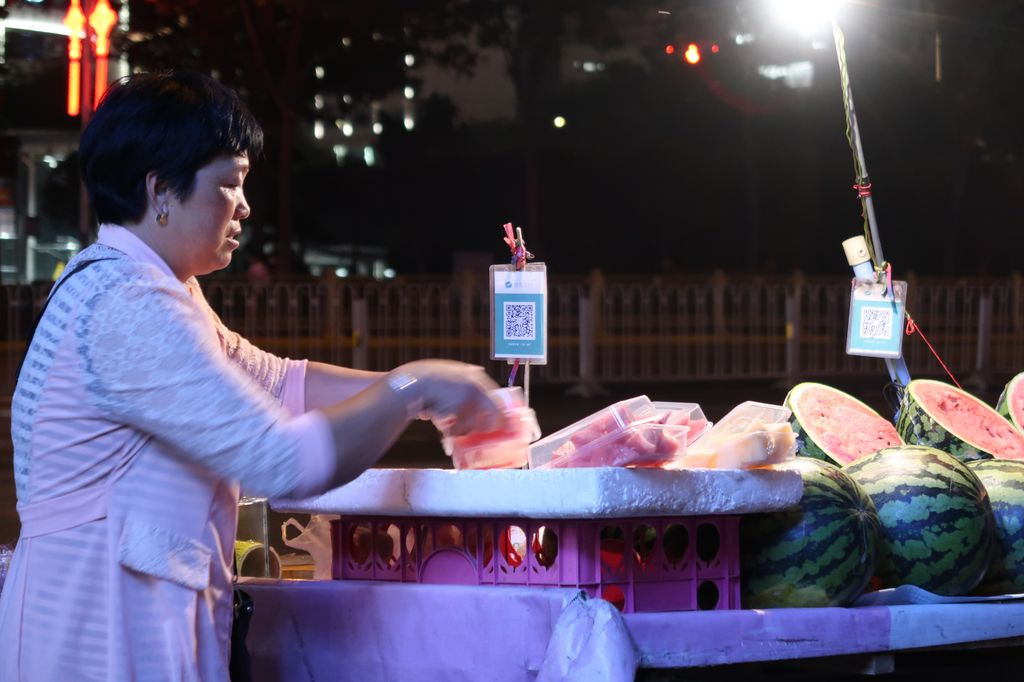
\includegraphics{images/20180622_wechat.JPG}
\caption{Puisqu'on vous dit que tout le monde utilise WeChat : même le
stand ambulant de fruits a son QR code.}
\end{figure}

Nous avons souvent eu du mal à nous faire comprendre en anglais, même
avec l'aide des applications de traduction hors-ligne. Les rares
personnes qui parlent anglais semblent souvent embêtées par nos
questions. Quelques contacts sont plus spontanés : des retraités ou bien
des enfants nous saluent par un "hello !" sympathique. Du coup pour
voyager, on s'en remet très souvent à des papiers écrits par les hôtes
des différentes auberges que nous présentons aux chauffeurs de bus ou au
passants. Mais à vrai dire, il n'y a là rien de bien curieux. Dans un
pays de 1400 millions d'habitants et donc de touristes potentiels, ce ne
sont pas les quelques millions de touristes étrangers qui comptent. Les
touristes en Chine, ce sont avant tout les chinois !

Nous avons également eu quelques tracas plus embêtants en Chine. Après
avoir visité la Cité interdite, nous avons été abordés par deux
Chinoises qui nous ont proposé de prendre un thé avec elles pour
discuter en anglais. La conversation nous a mis en confiance, mais
l'addition est salée, avec un prix plus de 20 fois supérieur à ce qui
aurait été raisonnable, que nous partageons avec elles. Très étonnés,
nous constatons sur internet que ce genre d'arnaque est arrivé à
d'autres touristes. Une autre aventure du même type concernait l'un de
nos trajets que nous devions faire en bus. Alors qu'on essayait
d'identifier notre arrêt de bus après un changement, un homme s'est
approché de nous, faisant mine de vouloir nous aider, puis nous a
affirmé que le dernier bus pour notre destination était déjà passé. Il
nous propose alors de nous emmener en voiture (c'était un trajet de 70
km) et à ce moment là, le bus est arrivé ! Belle technique de taxi pour
gagner des passagers...

Sur le plan de l'hygiène, autant dire que malgré les très nombreux
employés de nettoyage dans les rues ou devant chaque WC public, et le
nombre impressionnant de poubelles, c'est pas encore ça. On a bien
souvent vu jeter des emballages par terre sans problème. Pour les
toilettes, règle numéro 1 : amener son propre papier et savon aux
toilettes. Règle numéro 2 : travailler sa souplesse car, amateurs de
trônes confortables s'abstenir, ce sont presque toujours des toilettes à
la turque. Et deux constats étonnants : si il y a parmi les nombreuses
cabines un ou deux toilettes assis, on y trouvera des traces de
chaussures sur la cuvette. Et même s'il y a foule aux toilettes des
femmes, les cabines assises resteront inoccupées... Chez les enfants,
ceux en âge de parler ne portent plus de couches-culottes mais des
pantalons ouverts au niveau des fesses. Pourquoi ? Les parents leur font
faire leurs besoins dans les poubelles ou directement par terre sur le
trottoir !

\begin{figure}
\centering
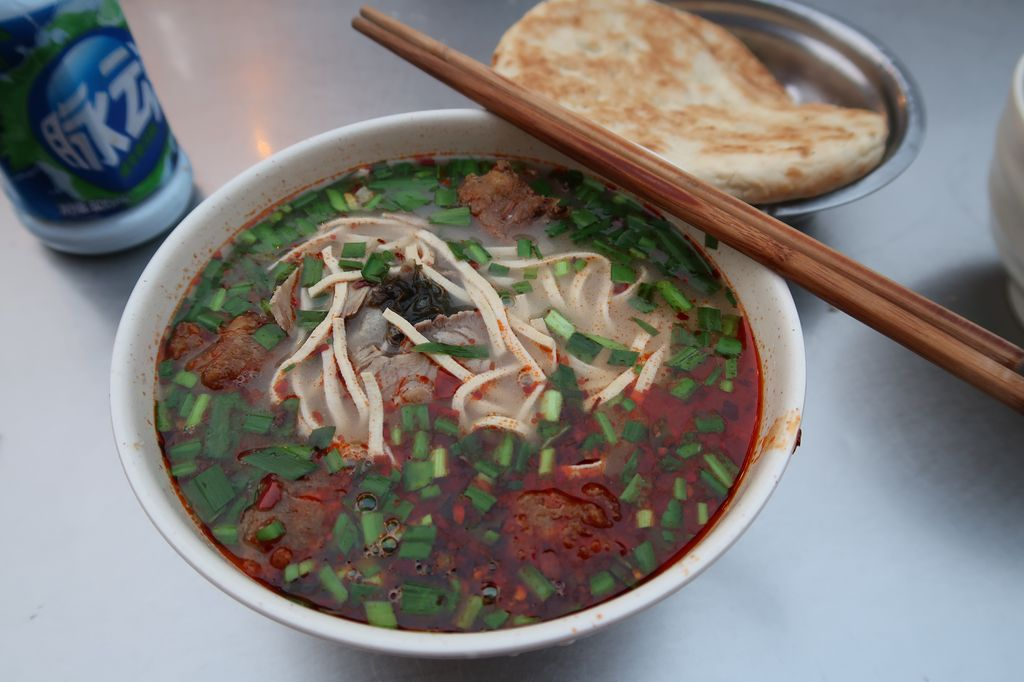
\includegraphics{images/20180622_soupe.JPG}
\caption{L'une des spécialités de Luoyang : une soupe de nouilles épicée
dans laquelle on jette des petits bouts de pain frais.}
\end{figure}

Mais concluons sur un point positif : nous avons beaucoup apprécié la
nourriture chinoise. Même en choisissant les plats au hasard, la grande
majorité de ce que nous avons pu manger était délicieux !

Un grand merci à Ruocong pour ses conseils avisés depuis Paris, et à
Longhui et Chen qui nous ont récupéré après ce tour de la Chine et aidé
à rejoindre l'aéroport.

A bientôt !

\emph{Florian et Elida}

\section{Konnichiwa!}

\emph{Lundi 25 juin 2018}

C'est après une très courte nuit dans l'avion qui nous amène de Shanghai
que nous posons pied sur l'archipel japonais, aussi appelé "la banane".
Une fois notre Japan Rail Pass en poche, des retrouvailles nous
attendent à Osaka, où nous sommes accueillis par Sorouch et Wakana.

\begin{figure}
\centering
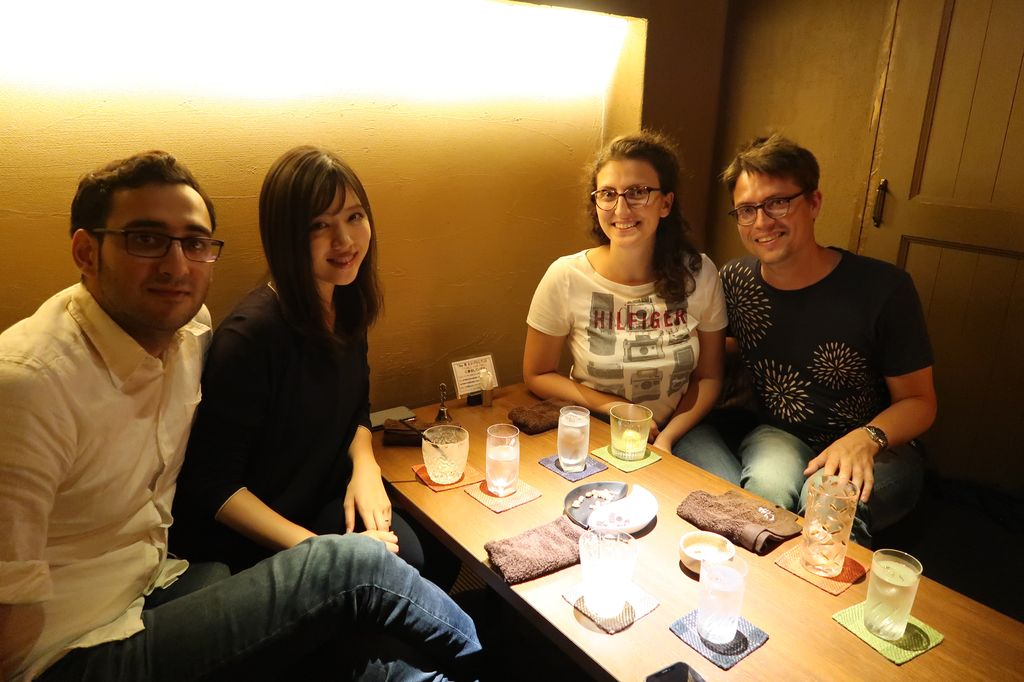
\includegraphics{images/20180625_osaka.JPG}
\caption{Nos hôtes dans le Kansai (région autour de Kyoto et Osaka),
Sorouch et Wakana, nous ont fait découvrir les spécialités d'Osaka.}
\end{figure}

Après deux courtes journées à Osaka, nous enchaînons avec un séjour dans
l'île la plus à l'ouest de l'archipel nippon, Kyushu.

Ce que nous vous raconterons bientôt, pour la suite de nos aventures au
Japon !

\emph{Florian et Elida}

\hypertarget{commentaires}{%
\subsection{Commentaires}\label{commentaires}}

\begin{itemize}
\item
  pythux, \emph{2018-06-25 20h46}

  C'est donc comme ça que ça s'écrit...
\item
  Elida, \emph{2018-07-10 03h43}

  Comme ça se prononce ! ;)
\end{itemize}

\hypertarget{quelques-jours-uxe0-kyushu}{%
\section{Quelques jours à Kyushu}\label{quelques-jours-uxe0-kyushu}}

En arrivant au Japon, nous nous sommes rendus compte que nous n'avions
pas de programme clair. La procédure de visa pour la Russie et la Chine
nous avait forcé à définir nos étapes avant de partir, donc nous sommes
arrivés un peu les mains dans les poches. Une fois passée l'euphorie de
retrouver mon pays de coeur et après un premier aperçu d'Osaka, nous
avons décidé de commencer notre séjour par l'île de Kyushu, l'île la
plus au sud de l'archipel nippon, que je ne connaissais pas du tout.

\begin{figure}
\centering
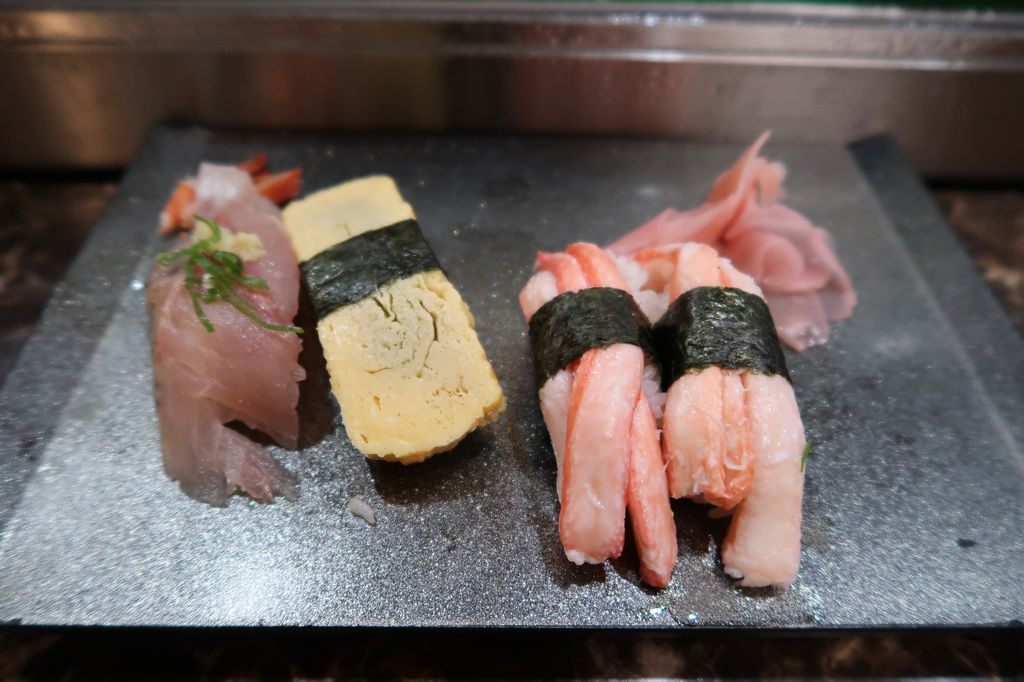
\includegraphics{images/20180709_sushi.JPG}
\caption{Après l'effort, le réconfort : de délicieux sushis mangés à
Osaka.}
\end{figure}

Au programme : la visite des villes de Fukuoka, Nagasaki et Kagoshima.
Nous avons pris nos quartiers à Fukuoka étant donné qu'avec
l'indispensable Japan Rail Pass on peut facilement (et économiquement)
prendre un train rapide vers les autres villes de l'île.

Fukuoka est la grande ville au nord de Kyushu. Nous avons profité des
conseils d'une expatriée et amoureuse du coin,
\href{http://www.benefukuoka.com/2015/12/fukuoka-conseils.html}{Béné no
Fukuoka}, pour découvrir les quartiers de cette ville découpée par des
canaux. La balade autour de la Fukuoka Tower a révélé une jolie plage
(depuis le temps qu'on avait pas mis les pieds dans le sable...) où les
poissons-volants offraient un drôle de spectacle au coucher du soleil.
Nous y avons mangé des \emph{Hakata ramen}, spécialité de pâtes
renommée, et y avons vu les préparatifs du festival Gion-Yamakasa. Il
s'agit d'une course de chars décorés de manière impressionnante,
opposant les différents quartiers de Fukuoka, portés à travers la ville
par des équipes d'hommes portant ce qui ressemble étrangement à des
"culottes" de sumo ; on vous laisse imaginer !

Nagasaki, c'est bien sûr la ville du drame atomique, mais aussi un port
de commerce qui a marqué l'histoire du Japon. Nous avons ainsi découvert
le complexe de Dejima, île artificielle installée en bordure de la ville
au 16ème siècle pour accueillir les portugais et hollandais de passage
(et circonscire fermement leur influence). L'île avait disparu avec le
temps, englobée par l'extension de Nagasaki, mais des fouilles ont
permis de la reconstituer avec un extraordinaire sens du détail. Quant
au musée de la bombe, il permet de se rendre compte de la gravité et de
l'horreur de l'évènement. Le parc de la paix, à côté, souligne le
message du musée de manière paisible.

\begin{figure}
\centering
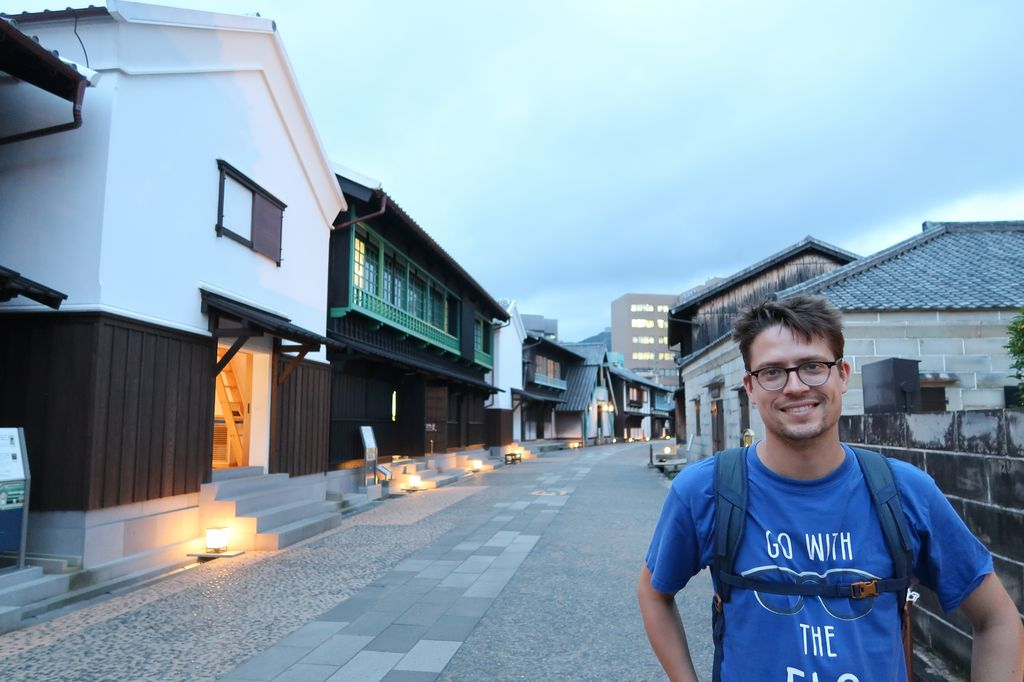
\includegraphics{images/20180709_dejima.JPG}
\caption{On peut vraiment passer des heures sur l'île reconstituée de
Dejima.}
\end{figure}

Enfin, Kagoshima. Une ville célèbre pour son rapport à l'île volcanique
avoisinante, Sakurajima. Peut-on vivre à côté d'un double-volcan avec
deux éruptions majeures au 20ème siècle à son actif, et qui crache des
cendres de façon quotidienne ? Il semblerait que oui. Les habitants vont
même jusqu'à collecter les cendres dans les sacs en plastique mis à
disposition par la ville (et que les touristes peuvent acheter
\^{}\^{}). Malheureusement, Sakurajima a gardé la tête dans les nuages
pendant notre journée à l'arpenter. L'île est un bel endroit pour
marcher et acheter des légumes, car le sol y est très fertile. On y a
d'ailleurs déjà fait pousser un radis de 30 kilogrammes...

\begin{figure}
\centering
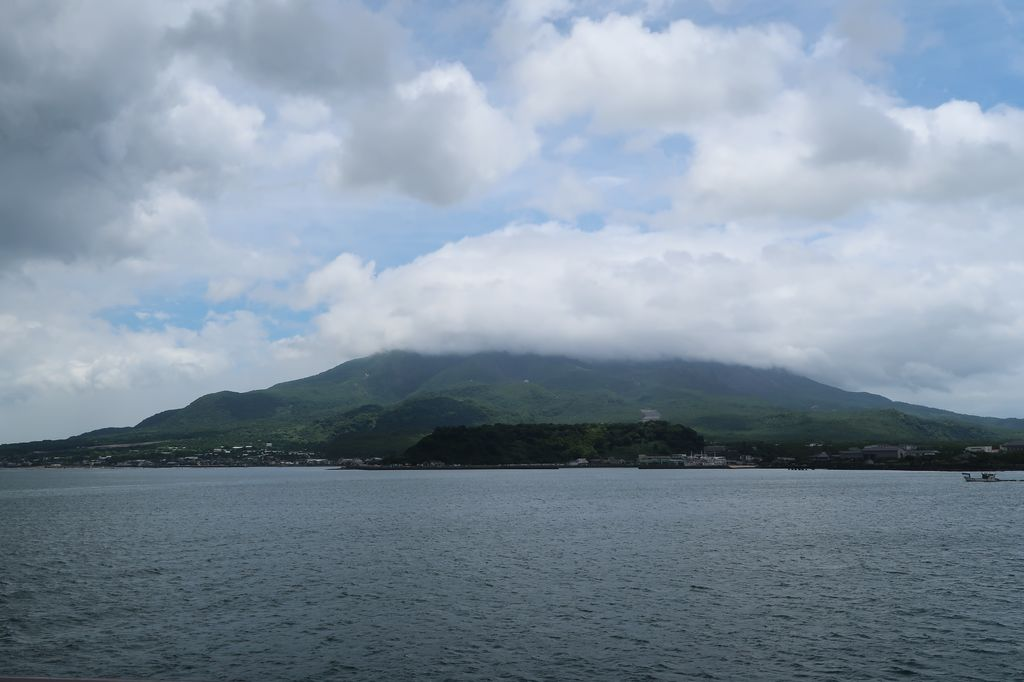
\includegraphics{images/20180709_sakurajima.JPG}
\caption{Île volcanique à l'horizon, capitaine !}
\end{figure}

Et voilà le récit de nos premiers jours au Japon, on vous laisse
maintenant découvrir les photos ci-dessous !

\emph{Florian et Elida}

\hypertarget{grand-uxe9cart-entre-tradition-et-gratte-ciels.}{%
\section{Grand-écart entre tradition et
gratte-ciels.}\label{grand-uxe9cart-entre-tradition-et-gratte-ciels.}}

Après notre sympathique escapade méridionale, et même si Flo l'a déjà
arpentée en long en large et en travers, nous sommes allés nous
installer à Tokyo. Chez Boris et Miwa plus exactement, qui nous ont
généreusement ouvert leurs portes dans le quartier du Tokyo Dome. Nous
avons récupéré en chemin ma cousine canadienne Marianne, qui est venue
partager un bout de vacances avec nous !

\begin{figure}
\centering
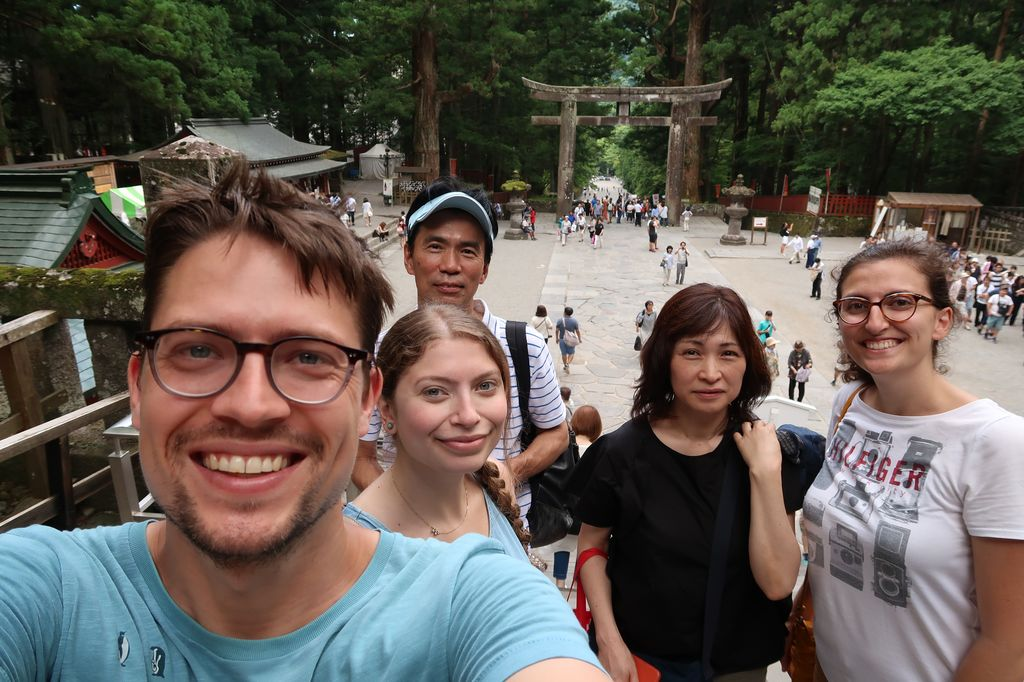
\includegraphics{images/20180710_nikko.JPG}
\caption{Excursion à Nikko avec Masaru et Keiko.}
\end{figure}

Mais après une soirée sous la chaleur de la capitale, nous voilà à
nouveau dans le train : Masaru, un ami de Flo, nous a concocté un
programme plein de surprises et de tradition pour le weekend. On le
retrouve à Mito, puis il nous fait passer par Oarai, ville de bord de
mer équipée d'un centre de recherche où Flo a passé une grosse partie de
sa seconde année au Japon. Après une très agréable soirée chez lui en
compagnie de Keiko, sa femme, nous partons le lendemain pour Nikko. On y
visite un sanctuaire impressionnant, le lac de Chuzenji, et en milieu
d'après-midi on s'installe dans un ryokan (hôtel traditionnel) pour
profiter des onsen (bains chauds) venant des sources volcaniques
avoisinantes. Pour ceux qui sont curieux il y a plein d'explications sur
le "rituel du onsen" partout sur internet, mais sachez que se baigner
dans son plus simple appareil dans des bassins fumants est très relaxant
et agréable, une fois passée l'appréhension initiale de laisser son
maillot de bain dans son sac ! Et le dîner gargantuesque qui suit la
baignade ne gâche aucunement le plaisir...

\begin{figure}
\centering
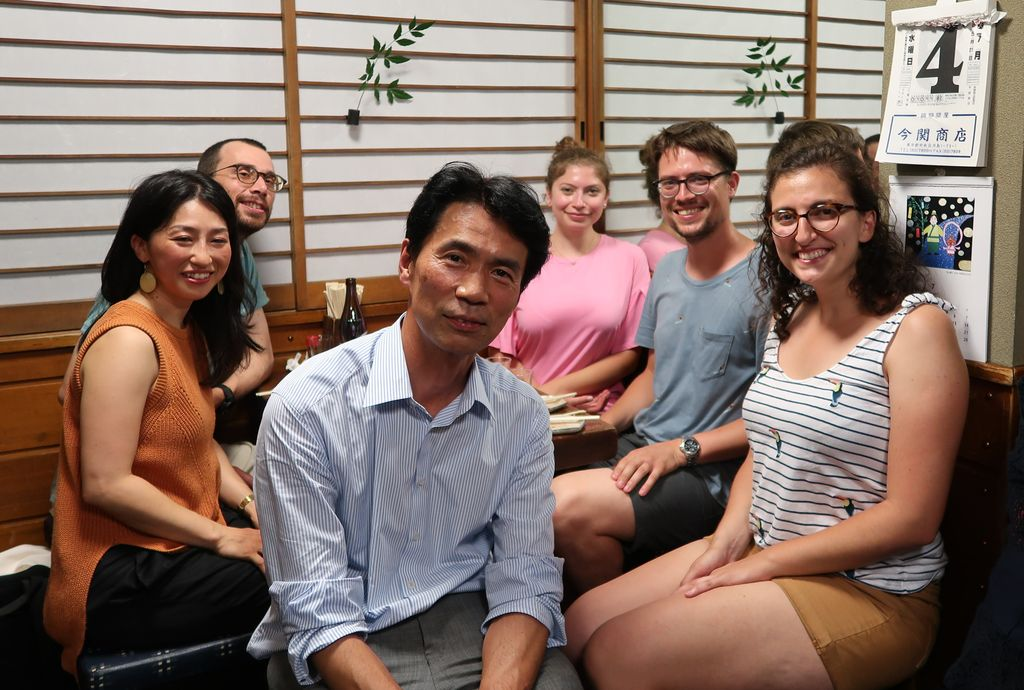
\includegraphics{images/20180710_boris.JPG}
\caption{Excellente soirée ponctuée de découvertes gustatives avec
Boris, Miwa et Masaru à Ginza.}
\end{figure}

De retour à Tokyo, on a arpenté les différents quartiers : Asakusa et
son temple, Ueno et son parc aux multiples musées, Harajuku et ses
magasins, Shinjuku et ses buildings imposants, la vibrante Shibuya, et
complètement à l'opposé le calme quartier de Yanaka et son immense
cimetière. Tout ce que mon imagination avait projeté sur cette ville, je
l'ai retrouvé. Modernité et tradition, j'ai l'impression qu'on se répète
mais c'est vraiment le ressenti que j'en garde. Modernité par l'aspect,
l'architecture, l'activité incessante, ces salarymen en chemise blanche
qui grouillent du matin au soir. Tradition par le caractère des gens,
les rapports extrêmement respectueux, les nombreux temples et
sanctuaires, et bien sûr la nourriture !

\begin{figure}
\centering
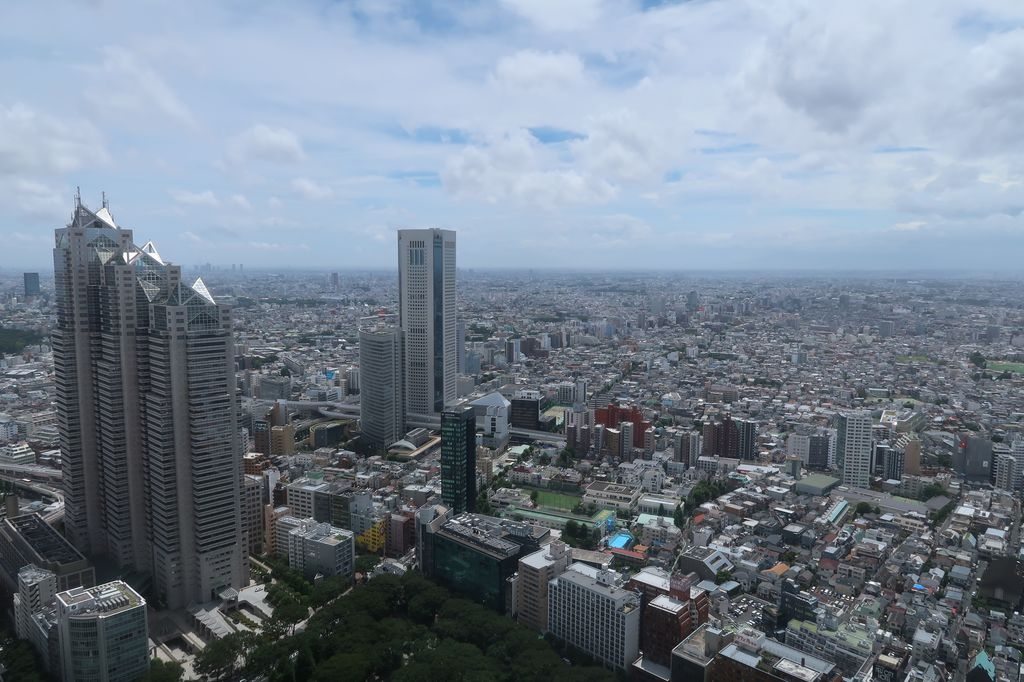
\includegraphics{images/20180710_shinjuku.JPG}
\caption{Tokyo vue d'en haut depuis le siège de la métropole à
Shinjuku.}
\end{figure}

Le temps d'une journée, nous avons aussi découvert la ville de Kamakura,
avec son grand Bouddha de bronze et le magnifique sanctuaire Hasedera.
On a même fini par une baignade dans les eaux tièdes mais agitées de
l'océan !

Notre prochaine étape nous mène à Kyoto, l'ancienne capitale. À suivre !

\emph{Elida et Florian}

\hypertarget{kyoto-autour-de-kyoto-et-hiroshima.}{%
\section{Kyoto, autour de Kyoto et
Hiroshima.}\label{kyoto-autour-de-kyoto-et-hiroshima.}}

Nous avons quitté Tokyo avec le Shinkansen. Ce train rapide, symbole
international du Japon, se distingue par ses retards incroyablement
faibles qui se comptent en moyenne \emph{en dizaines de seconde par
train}, tous trajets cumulés sur une année. Bien sûr, il faut préciser
que ce train rapide est également très cher (environ 110 euros pour 450
kilomètres en deux heures et demi pour un Tokyo - Kyoto).

Manque de chance, des pluies exceptionnelles ont perturbé le service
lors de notre trajet vers Kyoto. C'est donc avec plus de deux heures de
retard que nous arrivons à destination. En plus de dix ans de séjours au
Japon, je sais que c'est exceptionnel. Et malheureusement ces
inondations ont fait des victimes nombreuses dans l'ouest du Japon.
Pourtant, à Kyoto, la situation est sous contrôle. Mis à part la rivière
Kamo qui est en crue, nous ne détectons rien de particulier. D'ailleurs,
la chaleur est étouffante. La température est systématiquement au-dessus
de 30 degrés, l'air humide. Ce qui n'a pas empêché la pluie de nous
surprendre plus d'une fois.

\begin{figure}
\centering
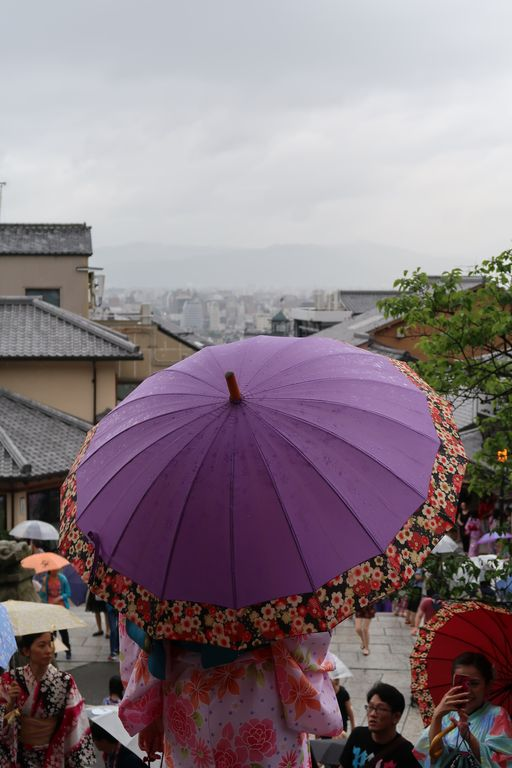
\includegraphics{images/20180716_kyoto.JPG}
\caption{Ambiance parapluie à Kyoto.}
\end{figure}

Nous retiendrons de Kyoto son ambiance à la fois rustique et branchée,
notamment entre Kawaramachi et Shijo, une rivière Kamogawa en crue ou
encore l'allure traditionnelle du quartier autour du Kiyomizudera (et
ses nombreux touristes), le temple de l'eau pure. Et le karaoké, qui
nous a donné l'occasion de chanter du Céline Dion par temps de pluie.

Cela dit, notre coup de coeur va à Arashiyama. A quelques dizaines de
minutes à l'ouest du centre de Kyoto, ce quartier à flanc de montagne
nous a fait découvrir de très beaux jardins et l'étonnante forêt des
singes. On peut y observer une tribu de macaques japonais de très près
(moment mignonitude devant les bébés) tout en profitant du cadre
idyllique.

\begin{figure}
\centering
\includegraphics{images/20180716_bambou.JPG}
\caption{Les spectaculaires bambous d'Arashiyama.}
\end{figure}

Notre plus beau coucher de soleil, ce fut au sommet du mont Inari auquel
on grimpe par l'intermédiaire du sanctuaire Fushimi Inari, le fameux
sanctuaire aux dix-mille portes Torii.

\begin{figure}
\centering
\includegraphics{images/20180716_inari.JPG}
\caption{Kyoto, vue de l'ouest.}
\end{figure}

Nous avons également profité du passage à Kyoto pour aller à Hiroshima,
à la faveur d'un lever aux aurores et du Shinkansen (de nouveau tout à
fait opérationnel). Nous y avons rendu visite à l'île de Miyajima (et y
voir une séance photo de mariage dans le sanctuaire local), vu un
célèbre Torii, mangé un okonomiyaki. On a fini par le mémorial de
l'attaque nucléaire de 1945. Pour nous remonter le moral après cette
triste visite, un petit MacDo à grande vitesse sur le chemin du retour
n'était pas de trop.

\begin{figure}
\centering
\includegraphics{images/20180716_torii.JPG}
\caption{Le Torii "les pieds dans l'eau" de Miyajima, au large
d'Hiroshima.}
\end{figure}

Pour finir, laissez-moi vous raconter comment on prend le bus à Kyoto
(et préparez vous à un sacré contraste avec la France) :

\begin{itemize}
\tightlist
\item
  on entre dans le bus par la porte arrière (et on sortira par celle de
  devant)
\item
  la tarification du trajet est soit un tarif unique, soit fonction de
  la distance, auquel cas cette distance est "mesurée" à l'aide d'un
  petit ticket papier que l'on prend en entrant et sur lequel est
  inscrit le numéro de la station initiale ; un écran informe ensuite
  les passagers des tarifs pour les différents points de départ
\item
  on cherche un endroit où s'asseoir
\item
  on s'étonne que le trajet soit commenté en direct par le chauffeur de
  bus, par exemple : "attention, virage en vue", "désolé, on doit
  s'arrêter au feu rouge", "c'est reparti !", ce qui anime le trajet !
\item
  une fois la destination en vue, on anticipe la descente et on se
  dirige vers la porte avant du bus
\item
  on prépare le montant exact demandé afin de le mettre dans une petite
  boîte à gauche du chauffeur
\item
  si l'on n'a pas pile la monnaie, on utilise la machine qui permet de
  faire du change (par exemple transformer un billet de 1000 yens en
  pièces de 500, 100 et 10 yens)
\item
  enfin, le chauffeur nous gratifie d'un \emph{arigato gozaimasu} bien
  senti lors du paiement et de la descente
\end{itemize}

Alors, ça donne pas envie de prendre le bus au Japon \^{}\^{} ?

\emph{Florian et Elida}

\hypertarget{des-alpes-japonaises-de-nagano-uxe0-la-bruxfblante-osaka}{%
\section{Des alpes japonaises de Nagano à la brûlante
Osaka}\label{des-alpes-japonaises-de-nagano-uxe0-la-bruxfblante-osaka}}

\emph{Lundi 16 juillet 2018}

Pour la suite de nos aventures, on a décidé de poser les valises
quelques jours à Nagano, plus en altitude, dans les "Alpes japonaises".
Effectivement, les chalets en bois et la fraîcheur (relative) de l'air
donnent à l'endroit des allures montagnardes, mais les reliefs sont
beaucoup plus...modérés. On s'installe à l'auberge de jeunesse
Moritomizu Backpackers, à deux pas de la gare, pour faciliter les
excursions. Nous y sommes accueillis à la japonaise : \emph{Alors voici
un plan de l'auberge, ici le premier étage, au-dessus le deuxième étage,
puis le troisième. Voici une maquette de votre futon, avec une petite
poupée qui vous représente, qui vous montre qu'il faut bien dormir entre
les deux draps.} Bien. Les doutes sur l'utilisation des draps ayant été
levés, on entame notre première excursion : Kanazawa.

\begin{figure}
\centering
\includegraphics{images/20180723_nagano.JPG}
\caption{Les petites Alpes japonaises, depuis le train.}
\end{figure}

A Kanazawa, on est accueillis par la porte Torii moderne de la gare, le
marché aux poissons en face, et par le prix des fruits, qui nous
surprend toujours ! Ils sont emballés un à un puis placés dans des
boîtes prêtes à poster (voir la photo dans la galerie). On se balade
ensuite dans l'ancien quartier des samouraïs où on visite la maison de
l'un d'eux, havre de tranquilité avec un jardin japonais d'où on a du
mal à partir. Après les samouraïs, les ninjas : le temple de Myoryuji a
été surnommé Ninja-dera, avec ses nombreuses cachettes, trappes
invisibles, escaliers camouflés et autres passages secrets supposés.
Sans oublier la chambre à thé, parce qu'en cas de siège il ne faut pas
oublier ses priorités ! On y a rencontré aussi Frankel, un touriste
d'Atlanta qui fera un bout de chemin avec nous. Après un court passage
au château de Kanazawa, la chaleur nous pousse plutôt vers le parc
Kenroku-en, où on regrette de ne pas être quelques mois plus tôt, à la
saison des cerisiers en fleurs... La journée se finit dans l'élégant
quartier des geishas, que nous n'aurons malheureusement pas le plaisir
de croiser sur notre chemin.

\begin{figure}
\centering
\includegraphics{images/20180723_kanazawa.JPG}
\caption{Le parc Kenroku-en.}
\end{figure}

Le lendemain, on part un peu plus en altitude, à Yamanouchi, où après
une agréable balade en forêt on arrive dans le domaine des macaques des
neiges. En hiver, ils y trouvent une source d'eau chaude pour se
baigner, mais en plein été ils sont surtout attirés par le repas apporté
par les employés du parc. N'empêche qu'ils sont nombreux et toujours
aussi fascinants à observer !

\begin{figure}
\centering
\includegraphics{images/20180723_singes.JPG}
\caption{Balade au milieu des macaques des neiges.}
\end{figure}

Sur le chemin du retour, on s'arrête à Obuse, la ville où le fameux
peintre Hokusai a passé une partie de ses vieilles années, et on
redécouvre ses oeuvres dans le petit musée qui lui est dédié. D'ailleurs
Hokusai a laissé une belle phrase concernant son art du dessin :

\begin{quote}
Depuis l'âge de 6 ans, j'avais la manie de dessiner la forme des objets.
Vers l'âge de 50 ans, j'avais publié une infinité de dessins, mais tout
ce que j'ai produit avant l'âge de 70 ans ne vaut pas la peine d'être
compté. C'est à l'âge de 73 ans que j'ai compris à peu près la structure
de la nature vraie des animaux, des herbes, des arbres, des oiseaux, des
poissons et des insectes. Par conséquent, à l'âge de 80 ans, j'aurai
fait encore plus de progrès ; à 90 ans, je pénétrerai le mystère des
choses ; à 100 ans, je serai certainement parvenu à un stade merveilleux
et, quand j'aurai 110 ans, tout ce que je ferai, un point, une ligne,
sera vivant.
\end{quote}

De retour à Nagano on arrive à la fin du jour au temple Zenko-ji, lieu
de pélerinage bouddhiste. La fin de journée donne un charme particulier
au lieu, où on se balade quasiment seuls. Une averse de pluie nous prend
au dépourvu mais ne fait qu'ajouter à l'ambiance un peu mystérieuse qui
règne.

\begin{figure}
\centering
\includegraphics{images/20180723_zenko.JPG}
\caption{Seuls au temple Zenko-ji.}
\end{figure}

En quittant Nagano, un peu à regret, on fait une escale à Matsumoto pour
y visiter son célèbre château noir, l'un des 12 châteaux originaux du
Japon. Le château a donc été rénové mais pas reconstruit de zéro, comme
c'est le cas de très nombreux châteaux détruits principalement pendant
la guerre du Pacifique. On profite de la disponibilité d'un adorable
guide volontaire qui nous raconte l'histoire et les secrets du château,
dans un récit ponctué de blagues et de jeux de mots... inattendus ! Ce
monsieur, d'un certain âge, a d'ailleurs systématiquement salué les
touristes étrangers sur notre passage en leur souhaitant la bienvenue
dans leurs langues respectives (allemand, espagnol, français, danois,
finnois, ...). Il nous a expliqué pouvoir échanger quelques mots dans
plus de vingt langues !

\begin{figure}
\centering
\includegraphics{images/20180723_matsumoto.JPG}
\caption{Devant le château du corbeau, surnom du château de Matsumoto.}
\end{figure}

De retour à Osaka, la chaleur ayant atteint son paroxysme, nous avons
pour la première journée opté pour un programme à l'opposé de tout ce
que nous avions fait jusque là : après une bonne heure de marche (pour
garder le rythme), on a enchaîné shopping/burgers/cinéma : presque
dépaysant ! Mais on ne pouvait pas partir sur une note si peu japonaise
: l'élégant château d'Himeji et ses marches dans tous les sens nous a
mis à l'épreuve avant la longue soirée qui nous attendait. On retiendra
que regarder la victoire de la France en finale de la coupe du monde
dans un pub irlandais à minuit à Osaka, entourés de gens de toutes
nationalités, est une expérience étonnamment riche en émotions.

\begin{figure}
\centering
\includegraphics{images/20180723_himeji.JPG}
\caption{L'élégant château d'Himeji, le château du héron blanc.}
\end{figure}

Enfin, avant de quitter Osaka et le Japon, une dernière expérience nous
a attirés : la visite du musée des nouilles instantanées. L'agréable
surprise a été la découverte de l'atelier, où après avoir décoré chacun
sa "cup" de nouilles, on la fait remplir de manière personnalisée, puis
sceller. On n'a pas encore goûté les nôtres, mais on vous en donnera des
nouvelles !

\begin{figure}
\centering
\includegraphics{images/20180723_noodles.JPG}
\caption{Atelier décoration de cup noodles, moment de retour en enfance
!}
\end{figure}

Après un dernier repas de sushis, il est temps de dire au-revoir au
Japon, que je suis heureuse d'avoir enfin découvert (après tout ce que
Flo me racontait tout le temps sur ce pays) et dont je garderai de très
bons souvenirs. Et de dire au-revoir à Marianne, que nous retrouverons à
la fin de notre séjour, au Canada, et qui nous a débarrassés d'un sac
d'affaires qui nous ont peu ou pas servies. On voyage encore plus léger
désormais !

Merci mille fois à tous nos hôtes franco-japonais, avec qui nous avons
passé de très agréables moments. A bientôt pour les prochaines
aventures, dans l'hémisphère Sud cette fois...

\textbf{bonus} Et voici la carte récapitulative de nos destinations au
Japon :

\begin{figure}
\centering
\includegraphics{maps/Japon.png}
\end{figure}

\emph{Elida et Florian}

\hypertarget{arrivuxe9e-au-pays-des-mille-oiseaux}{%
\section{Arrivée au pays des mille
oiseaux}\label{arrivuxe9e-au-pays-des-mille-oiseaux}}

\emph{Dimanche 22 juillet 2018}

Changement d'hémisphère, de saison, perte de plus de 20 degrés et de 4
heures d'ensoleillement par jour, shorts rangés, de l'anglais partout
autour de nous (mais avec un accent bizarre quand même) : pas de doute,
on est bien arrivés en Australie ! Et on a été accueillis royalement par
Svenja et Rémi, expatriés dans le pays du kangourou depuis de nombreuses
années, qui nous ont ouvert leurs portes à Sydney.

\begin{figure}
\centering
\includegraphics{images/20180724_australie.jpg}
\caption{Avec nos hôtes, excursion sur la Central Coast.}
\end{figure}

Et l'Australie fait déjà son petit effet sur nous : certes c'est
l'hiver, mais cela n'empêche pas les petits déjeuners sur la terrasse,
avec des perroquets aux couleurs vives qui viennent réclamer un bout de
pain, les balades sur la plage à observer les surfeurs, et même le
passage de quelques baleines à l'horizon...

On vous raconte ça très vite !

\begin{figure}
\centering
\includegraphics{images/20180724_plage.jpg}
\caption{Coucher de soleil sur Bouddi Beach.}
\end{figure}

\emph{Elida et Florian}

\hypertarget{on-na-jamais-uxe9tuxe9-autant-uxe0-la-plage-en-hiver}{%
\section{On n'a jamais été autant à la plage en
hiver}\label{on-na-jamais-uxe9tuxe9-autant-uxe0-la-plage-en-hiver}}

Sur les conseils avisés de nos hôtes, Svenja et Rémi, nous avons exploré
différents points touristiques de la région de Sydney. Si on voulait
résumer notre programme en un seul mot, ce serait \textbf{plage}. Malgré
l'hiver, nos déplacements nous ont tous amené au point de rencontre
entre le sable, les vagues et le ciel dont la Nouvelle-Galles du Sud
regorge.

L'une des premières étapes sur notre chemin a été la découverte du
quartier de Darlinghurst, où nous logeons. Comme Elida l'évoquait à
travers le titre de l'\href{/arrivee-australie.html}{article précédent},
on croise toutes sortes d'oiseaux à Sydney, bien plus que ce dont nous
avons l'habitude. Que ce soient les cacatoès, les kookaburras ou les
"petits gris", les derniers descendants des dinosaures nous ont séduits
ici ! Quoi de plus agréable que de prendre le petit déjeuner avec des
perroquets ?

\begin{figure}
\centering
\includegraphics{images/20180726_perroquets.JPG}
\caption{Le gang des trois perroquets, prêts à tout pour obtenir de la
mie de pain au petit déjeuner.}
\end{figure}

Pour en revenir au sujet, nous avons donc découvert les endroits
suivants :

\begin{itemize}
\tightlist
\item
  Bondi beach : la plage "légendaire" de l'été australien, mais qui
  offre également une belle promenade en bordure de mer pour admirer le
  relief ; on a même eu la chance d'y apercevoir des baleines !
\item
  Watson's bay : l'un des caps qui délimite la baie de Sydney par le
  sud, là aussi l'occasion de marcher le long de jolis sentiers
\item
  Manly : nommée par le capitaine Arthur Philipp en raison de la
  virilité des locaux, c'est l'anti-Watson's bay, duquel nous avons
  marché de crique en crique et à travers le Sydney Harbour National
  Park, jusqu'à atteindre Spit Bridge (une balade mémorable qu'on a
  terminé à la lampe torche...)
\item
  Balmoral : abritée dans la baie de Sydney, cette partie de la côte
  offre des vues magnifiques sur le centre-ville et son port
\end{itemize}

Ces promenades nous ont permis de mieux comprendre ce qui fait la
spécificité et l'art de vivre de Sydney : ville cosmopolite, moderne et
riche d'histoire, mais surtout très près de sa nature et de sa faune
abondante. De nombreuses mesures semblent d'ailleurs constamment mises
en œuvre pour protéger la nature : panneaux signalant les interdits mais
aussi les types de plantes, poubelles avec tri et recyclage, zones de
régénération du "bush" où l'on se nettoie les chaussures pour éviter de
transporter des spores exogènes, zones de végétation replantée, plages
où les chiens ne sont pas autorisés... Et cela a l'air de marcher : on
trouve très peu de déchets abandonnées, les côtes sont très propres avec
une faune et une flore très riches et variées et donc un véritable
bonheur à explorer.

\begin{figure}
\centering
\includegraphics{images/20180726_bush.JPG}
\caption{Le bush australien par l'exemple.}
\end{figure}

Le temps d'un week-end, Svenja et Rémi nous ont emmenés un peu plus au
nord de Sydney, sur la Central Coast. La route donne le ton : très
rapidement à la sortie de la ville on se retrouve sur des voies
découpées au milieu de la montagne, puis nous commençons à apercevoir à
chaque virage le scintillement des vagues, et des plages plus belles les
unes que les autres. On s'arrêtera à des plages aux noms évocateurs :
Pearl Beach, Copacabana,... Les balades sur le sable sont très agréables
même si parfois un peu fraîches (n'oublions pas qu'on est en plein hiver
ici), et la lumière du coucher de soleil sur la côte découpée du Bouddi
National Park nous émerveille.

Voilà pour ce premier aperçu de notre voyage en Australie, on continue
bientôt pour un road-trip sur la Great Ocean Road !

\emph{Florian et Elida}

\hypertarget{en-route-sur-la-great-ocean-road}{%
\section{En route sur la Great Ocean
Road}\label{en-route-sur-la-great-ocean-road}}

\emph{Mardi 31 juillet 2018}

Même si cela ne faisait pas partie de nos plans initiaux (qui étaient en
fait inexistants, avouons-le), nous avons passé les derniers jours à
parcourir un bout d'Australie en voiture. Et cela a été une très belle
expérience (au prix d'encore plus de CO2 sous forme de billets d'avion).

Alors, c'est quoi cette Great Ocean Road ? C'est une route
\emph{scénique} d'environ 300 kilomètres qui, comme son nom le suggère,
serpente le long de l'océan entre Geelong, près de Melbourne, jusqu'à
Warrnambool, vers l'ouest. Construite par des hommes qui avaient servi
l'Australie pendant la première guerre mondiale (et qu'il fallait bien
remettre au boulot), la route a été voulue comme un monument à la
mémoire de tous ceux qui sont tombés durant le conflit.

\begin{figure}
\centering
\includegraphics{images/20180731_greatoceanroad.JPG}
\caption{Sous la porte d'entrée de la Great Ocean Road.}
\end{figure}

Certains la visitent en une journée express, nous on avait la chance
d'avoir plein de temps, on l'a donc parcourue en cinq jours qui peuvent
se découper en quatre étapes. Et on en a pris plein les yeux !

\begin{figure}
\centering
\includegraphics{maps/great_ocean_road.png}
\end{figure}

\hypertarget{de-geelong-uxe0-lorne}{%
\subsection{De Geelong à Lorne}\label{de-geelong-uxe0-lorne}}

La première partie du trajet nous a menés par Geelong que nous n'avons
vue que très rapidement sous une météo capricieuse, puis Torquay et sa
fameuse Bells Beach, siège de compétitions de surf. Nous nous sommes
ensuite arrêtés à Anglesea, où nous avons rencontré pour la première
fois de charmants kangourous, qui vivent leur vie au milieu des
golfeurs. Après un dernier arrêt au phare de Aireys Inlet et ses vues
magnifiques, nous avons fini la journée à Lorne, petite ville
touristique coincée entre la côte et les denses forêts du Otway National
Park. Nous avons gardé une journée entière pour explorer Lorne, où on
trouve de nombreuses occasions d'admirer la nature avoisinante avec pas
moins de dix chutes d'eau accessibles par des sentiers forestiers. On y
a aussi aperçu une baleine depuis le débarcadère !

\begin{figure}
\centering
\includegraphics{images/20180731_erskinefalls.JPG}
\caption{Erskine Falls, l'une des cascades recommandées par l'office du
tourisme local.}
\end{figure}

\hypertarget{de-lorne-uxe0-apollo-bay}{%
\subsection{De Lorne à Apollo bay}\label{de-lorne-uxe0-apollo-bay}}

Le moment clé de cette portion de la route aura incontestablement été
l'observation des koalas dans la forêt d'eucalyptus à Kennett River. On
a appris qu'il fallait beaucoup de patience et de concentration pour
repérer ces boules de poils grises qui passent leur temps à dormir en
haut des eucalyptus, mais ça a payé : en remontant la Grey River Road,
nous avons eu la chance d'en compter au moins sept ! Avec en prime
encore et toujours des vues magnifiques sur la forêt et l'océan, une
fois arrivés en haut de la montagne. A Apollo Bay, le Marriner's lookout
nous a offert de magnifiques paysages avec des pâturages d'un côté, et
l'interminable plage de l'autre, de quoi bien finir la journée !

\begin{figure}
\centering
\includegraphics{images/20180731_apollobay.JPG}
\caption{La baie d'Apollon au soleil couchant.}
\end{figure}

\hypertarget{dapollo-bay-jusquuxe0-princetown}{%
\subsection{D'Apollo bay jusqu'à
Princetown}\label{dapollo-bay-jusquuxe0-princetown}}

Après une balade au sanctuaire marin de Marengo Reefs, où nous espérions
croiser la colonie de phoques qui séjourne par là (mais qui ne se sont
pas montrés ce jour-là), l'excursion de la journée nous a amené à Cape
Otway, l'un des premiers phares construits en Australie. L'histoire du
coin est en effet riche en naufrages, de nombreux vaisseaux en
provenance d'Angleterre ayant été victimes des récifs qui s'étendent
jusqu'à 8 km des côtes par endroits. Les guides nous ont également
sensibilisés à la cause aborigène, qui reste aujourd'hui encore un point
de conflit interne en Australie.

\begin{figure}
\centering
\includegraphics{images/20180731_capeotway.JPG}
\caption{Le phare de Cape Otway.}
\end{figure}

\hypertarget{de-princetown-uxe0-warrnambool}{%
\subsection{De Princetown à
Warrnambool}\label{de-princetown-uxe0-warrnambool}}

Sans aucun doute le segment le plus fréquenté de cette route
touristique. De nombreux arrêts ont été aménagés dû aux belles
formations rocheuses en bordure de côte que l'on y trouve. La plus
célèbre, ce sont les Douze Apôtres, des roches dressées dans la mer qui
les érode peu à peu (et qui sont sept, non-pas douze !). La journée a
été ponctuée par des orages et des averses de grêle, pendant lesquels on
attendait sur le parking la prochaine éclaircie pour nous permettre de
jeter un coup d'œil aux sites... On a donc quand même pu s'arrêter à
Loch Ard Gorge, London Arch, The Grotto, Bay of Islands, pour ne citer
que les principaux. On a globalement fini trempés, mais la lumière au
moment des accalmies était très belle, et on a même gagné quelques
arc-en-ciels en bonus !

\begin{figure}
\centering
\includegraphics{images/20180731_douzeapotres.JPG}
\caption{Les Douze Apôtres en fin de journée.}
\end{figure}

Après avoir fini de parcourir la Great Ocean Road, nous avons également
fait une brève halte à Melbourne. Nous n'avons pas pu nous y attarder,
mais nous garderons un bon souvenir de la visite guidée de la
bibliothèque d'état du Victoria, dans les tréfonds de laquelle
sommeillent un pendule de Foucault (sans pendule), un ascenseur à
éléphant et des catacombes...

\begin{figure}
\centering
\includegraphics{images/20180731_melbourne.JPG}
\caption{On comprend mieux la solide réputation de ville de street art
qu'a Melbourne quand on arpente ses ruelles.}
\end{figure}

Nous retournons maintenant passer nos dernières journées australiennes à
Sydney, avant de nous envoler pour la Polynésie Française.

\emph{Florian et Elida}

\hypertarget{commentaires}{%
\subsection{Commentaires}\label{commentaires}}

\begin{itemize}
\item
  ZRC, \emph{2018-07-31 16h13}

  Mais, je n'aperçois pas ces fameux koalas que vous avez vus !\\
  Et je me permets de signaler que la star de la photo 2 n'est pas un
  végétal...
\item
  Florian LB, \emph{2018-08-01 02h24}

  Salut Ruocong ! Quelle lecture attentive ! Concernant les koalas, il
  semblerait qu'Elida prépare un billet spécial sur la faune
  australienne. Peut être y figureront ils ? Quant au végétal qui n'en
  est pas un, je serais ravi que tu éclaire ma lanterne proverbiale.
  C'est quoi ?
\item
  ZRC, \emph{2018-08-01 12h32}

  Il me semble que ce sont des champignons (du règne des Fungi, ou
  Mycètes), non ? Visuellement les recherches semblent pointer vers
  Trametes versicolor.
\item
  Florian LB, \emph{2018-08-02 10h41}

  Ça y ressemble en effet ! Je ne savais pas que les champignons étaient
  un règne à part, voilà pour ma culture générale...
\item
  Thibaud, \emph{2018-08-07 11h16}

  Je dirais que le mont éléphant ressemble à un éléphant, mais ça paraît
  trop simple o\_O\\
  Vous dormiez où sur la route ? En auberge ?
\item
  Florian LB, \emph{2018-08-08 08h01}

  Haha ben on est d'accord avec toi pour l'explication, même si on a pas
  de source plus fiable !\\
  On a pris des locations Airbnb et une auberge de jeunesse sur le
  chemin.
\item
  Franck Mazas, \emph{2018-08-14 10h50}

  La reconversion en coastal engineer me paraît inévitable.
\item
  Florian LB, \emph{2018-08-16 07h35}

  Haha ce n'est pourtant pas la seule possibilité...
\end{itemize}



\hypertarget{des-kangourous-mais-pas-que}{%
\section{Des kangourous, mais pas que
!}\label{des-kangourous-mais-pas-que}}

\emph{Jeudi 02 août 2018}

Dès le premier jour, ce qui nous a le plus marqué en Australie, c'est
les oiseaux. On les entend chanter du soir au matin, où que ce soit y
compris au cœur des grandes villes. Les petits loriquets viennent
réclamer du pain sur la terrasse le matin, le kookabura fait office de
réveil aux aurores avec son chant qui ressemble à un rire moqueur, les
cacatoès font un boucan d'enfer dans les parcs, les mouettes restent
fidèles à elles-mêmes et tournent autour des terrasses de \emph{fish and
chips} et les ibis font les poubelles avec leur long bec... On a aussi
croisé des pies dont le cri ressemble à R2-D2, des dindons sauvages dans
les forêts, de beaux perroquets à Kennett River, et même une chouette en
plein centre de Sydney !

Pour ce qui est des animaux terrestres, les incontournables kangourous
et leurs petits frères les wallabies se sont avérés très curieux, et les
koalas nous ont attendri, une fois qu'on a réussi à les voir !

\begin{figure}
\centering
\includegraphics{images/20180802_kangourou.JPG}
\caption{Attention aux kangourous.}
\end{figure}

Comme les images valent mieux que mille mots, voici un condensé de ces
magnifiques animaux. On n'a pas réussi à trouver le nom de tous ces
animaux (surtout les oiseaux...), alors pour les ornithologues parmi
vous, n'hésitez pas à nous instruire :)

\emph{Elida et Florian}

\hypertarget{commentaires}{%
\subsection{Commentaires}\label{commentaires}}

\begin{itemize}
\item
  Franck Mazas, \emph{2018-08-14 10h47}

  Emu, en bon français, c'est plutôt émeu. Mettons ça sur le compte de
  l'émotion !\\
  Je suggérerais bien le développement d'un script Python pour la
  reconnaissance automatique des volatiles à partir d'une base de
  données, mais j'aurais trop peur que les pythons bouffent les oiseaux,
  c'est bien connu.
\item
  Florian LB, \emph{2018-08-16 07h39}

  Aaaah c'est pour ce genre de précision qu'on apprécie tes commentaires
  Franck ! Merci, je vais essayer de corriger ça. Quant au script
  python, il va devoir attendre je suis encore en vacances pour 3 mois
  :)
\item
  Didier VEZINET, \emph{2018-08-29 20h17}

  Le truc ou tu sêches c'est pas une variété de héron ?\\
  Ils sont trop mignons les wallabies :-)
\item
  Florian LB, \emph{2018-09-02 00h07}

  Des hérons... possible !\\
  C'est sûr que les wallabies et les kangourous, on les aurait bien
  approchés de plus près. Mais ils sont trop timides !
\end{itemize}

\hypertarget{premiers-pk-et-premiuxe8res-uxeeles-en-polynuxe9sie-franuxe7aise}{%
\section{Premiers Pk et premières îles en Polynésie
Française}\label{premiers-pk-et-premiuxe8res-uxeeles-en-polynuxe9sie-franuxe7aise}}

\emph{Vendredi 10 août 2018}

Cela fait maintenant une bonne semaine que nous sommes arrivés en
Polynésie Française. Je faisais partie des gens qui confondaient
\emph{Tahiti} avec \emph{Polynésie Française}. Après quelques jours ici,
j'ai bien pris conscience de la gaffe ! Réduire la Polynésie à une seule
île, ça ne marche tout simplement pas.

Nos premiers pas sur les îles se passent à Tahiti et Moorea.

\hypertarget{mapid}{}

Que dire de Tahiti alors ? Même si c'est le centre administratif de la
Polynésie Française, l'île elle-même est loin de l'image paradisiaque
associée à d'autres îles de l'archipel. Nous retiendrons quand même
quelques détails savoureux:

\begin{itemize}
\tightlist
\item
  il y a des chiens et des poules au bord de toutes les routes
\item
  tout le monde se lève avant 7 heures du matin (et se couche en
  conséquence)
\item
  quand on fait le tour de l'île, on trouve régulièrement des bornes
  appelées Pk, point kilométrique, qui permettent efficacement
  d'indiquer les localisations des points d'intérêt
\item
  on trouve des roulottes, sortes de food-truck immobilisés avec sièges
  et tables, un peu partout sur l'île et on y mange le plat national, le
  \emph{poisson cru coco}
\item
  les habitants de l'île sont tous très détendus, on est loin de
  l'esprit si commercial dont a l'habitude dans les lieux touristiques
  qu'on a fréquentés (même si évidemment le tourisme est ici aussi une
  manne)
\item
  on peut également faire de la randonnée sur l'île car le relief
  volcanique est très accidenté (nous en avons profité et sommes montés
  à la cascade de Loti)
\item
  il n'y a pas de plages partout, contrairement à ce que l'on pourrait
  penser, il faut un peu chercher pour les trouver (mais elles sont
  souvent magnifiques)
\end{itemize}

\begin{figure}
\centering
\includegraphics{images/20180810_tahiti.JPG}
\caption{En parlant de plages...}
\end{figure}

Nous retrouvons à Tahiti Guillaume et Camille avec qui nous voyagerons
pour les prochaines semaines.

Plus que Tahiti, c'est à Moorea que va notre coup de coeur de la
première semaine en Polynésie. A moins d'une heure en bateau de Tahiti,
et sur une surface bien plus petite, nous y avons passé quatre belles
journées. Cela est notamment dû à l'accueil parfait que nous a réservé
Laura, voyageuse espagnole en séjour longue durée à Moorea, dénichée via
AirBnb. Laura nous aura tout appris sur les attraits de l'île, y compris
comment préparer un poisson perroquet acheté en direct à son pêcheur
pour un barbecue réussi !

\begin{figure}
\centering
\includegraphics{images/20180810_moorea_laura.JPG}
\caption{Notre hôte à Moorea, Laura, le jour de notre départ.}
\end{figure}

Nous découvrons avec plaisir les différentes activités typiques des îles
polynésiennes : snorkeling avec les raies, mais aussi les requins (oui,
ça fait bizarre au début), tour de l'île tous les deux en scooter (mais
sans jamais dépasser quarante-cinq kilomètres à l'heure !), détente à la
plage de rêve de Temae, excursion pour faire du snorkeling et entendre
le chant des baleines. Ou encore visite de l'usine de jus de fruit
Rotui, qui fait la célébrité (et parfois la jalousie) de Moorea dans les
autres îles, observation astronomique depuis la terrasse quand le ciel
est clair et que s'ouvre au-dessus de nous la voie lactée. On découvre
aussi la météo qui peut être changeante : on passe facilement d'une
grosse averse qui fait mal (mais ne dure que dix minutes) au grand
soleil ! Et bien sûr les couchers de soleil sur la mer, dont on ne se
lasse pas...

Voilà donc les premières impressions d'ici. On enchaîne très bientôt
avec quatre jours à Bora-Bora, île du tourisme de luxe si l'on fait
confiance aux réputations !

\emph{Florian et Elida}

\hypertarget{les-uxeeles-sous-le-vent-uxe7a-secoue}{%
\section{Les Îles-Sous-Le-Vent, ça secoue
!}\label{les-uxeeles-sous-le-vent-uxe7a-secoue}}

\emph{Lundi 20 août 2018}

Comme on nous l'a dit pendant une excursion en bateau, les Polynésiens
ne le sont pas pour rien : nous avons constaté pendant la suite de notre
séjour toute l'étendue de leur polyvalence, et celle de leurs îles. Tour
d'horizon de ce que nous avons vu et fait dans les Îles-sous-le-vent.
Pour ceux qui ne sont pas familiers du terme, l'archipel où nous avons
voyagé s'appelle l'archipel de la Société. Vers l'Est se trouvent Tahiti
et Moorea, les Îles-du-vent, et vers l'Ouest se trouvent principalement
Bora-Bora, Maupiti, Raiatea, Tahaa et Huahine. Hormis cette dernière (où
nous n'avons pas mis les pieds), nous avons arpenté ces îles en long, en
large et en travers !

\begin{figure}
\centering
\includegraphics{maps/Polynesie2_1.png}
\caption{Arrivée à Bora-Bora et son lagon sublime !}
\end{figure}

Attention, long article en vue mais on vous met plein de photos, on a eu
du mal à choisir !

\hypertarget{bora-bora}{%
\subsection{Bora-Bora}\label{bora-bora}}

\begin{figure}
\centering
\includegraphics{images/20180820_boraselfie.JPG}
\caption{Arrivée à Bora-Bora et son lagon sublime !}
\end{figure}

Et nous avons commencé par Bora-Bora, dont le nom était porteur de plein
d'images de carte postale et aussi source d'inquiétudes. En effet, les
prix étant significativement plus élevés sur cette île, nous avions fait
le plein de courses à Tahiti (et même depuis l'Australie !). Ce qui
marque en premier quand on survole Bora, c'est la forme de ses
montagnes, très singulière. Ensuite, c'est pendant la traversée en
bateau pour rejoindre l'île principale depuis le motu (îlôt de sable) de
l'aéroport que le bleu du lagon nous impressionne : pour le coup on sait
qu'on y est, dans la carte postale !

Et puis Bora, c'est synonyme d'hôtels de luxe, avec les fameux bungalows
au-dessus de l'eau. On voit bien les bungalows quand on fait le tour du
lagon, mais on croise moins leurs locataires, qui doivent donc être
assez peu nombreux et sans doute cantonnés aux activités proposées par
leur hôtel. Ce qui fait qu'on a été agréablement surpris. On s'attendait
à se retrouver à Saint-Tropez et finalement on aura côtoyé surtout des
polynésiens ! Et tout particulièrement la famille qui nous a reçu tous
les quatre : l'accueil chaleureux et généreux de Mataha, JP et les
filles nous a fait nous sentir comme à la maison. On se souviendra
longtemps de Tiheni, 4 ans, qui joue au coiffeur avec les garçons : "tu
veux quoi comme coupe ? Bôgosse ?" :D

\begin{figure}
\centering
\includegraphics{images/20180820_mataha.JPG}
\caption{Notre hôte à Bora-Bora : Mataha (et sa famille).}
\end{figure}

Après une première journée à faire le tour de l'île en vélo (34 km),
histoire de mieux comprendre où on est (avec une flotte de vélos à un
disque et sans freins et un tricycle, je vous laisse imaginer la galère,
heureusement que c'est presque tout plat !), on a enchaîné le lendemain
avec le tour de l'île en bateau. Comment ne pas profiter du lagon, un
des plus beaux atouts de l'île : on a commencé par nager avec une
impressionnante raie manta, puis nous avons retrouvé nos copines les
raies pastenagues et les requins à pointe noire, puis une exploration du
jardin de corail avec ses bancs de poissons colorés et ses coquillages
presque fluorescents... Le tout entrecoupé d'un délicieux repas
polynésien, en phase avec la nature : plats et assiettes en feuilles de
bananier tressées, "Les fourchettes ? Vos doigts. Les couteaux ? Vos
dents !".

Pendant une journée pluvieuse, on s'est baladés avec JP qui nous a
raconté plein de choses, dont l'utilisation du noni, un fruit qui sent
vraiment très mauvais, exporté aux Etats-Unis pour en faire des
jus-qui-guérissent-tout. On parle aussi de l'histoire des bunkers qui se
trouvent aux quatre coins de l'île (aujourd'hui encore utilisés comme
refuge en cas de cyclone), construits par les américains pendant la
seconde Guerre Mondiale après l'attaque de Pearl Harbor. Ils ont utilisé
Bora comme base et y ont construit le premier aéroport de Polynésie.

On s'est aussi lancés dans une activité peu pratiquée à Bora : la
randonnée. L'ascension du Mont Ohue, à plus de 660 mètres d'altitude,
nous a donné bien du fil à retordre. 3 heures de montée, autant de
descente, un balisage au scotch gris dans les arbres, des passages avec
des cordes et le tout sur un terrain glissant au vu des pluies de la
veille...et on oublie toutes les peines une fois arrivés en haut : la
vue est à couper le souffle (et non, c'est pas que à cause de la fatigue
!), on a du mal à vouloir redescendre. D'ailleurs, on paiera nos
exploits pendant 3 jours avec de bonnes courbatures, qu'on traînera
jusqu'à l'île suivante : Maupiti !

\begin{figure}
\centering
\includegraphics{images/20180820_borarando.JPG}
\caption{La vue depuis le sommet de Bora-Bora !}
\end{figure}

\hypertarget{maupiti}{%
\subsection{Maupiti}\label{maupiti}}

Maupiti a un charme bien à elle, et très différent de Bora. A commencer
par sa taille : 10 kilomètres de circonférence, un petit millier
d'habitants, qui ont voté par référendum l'interdiction des hôtels sur
l'île. Ils gèrent donc le tourisme sur leur île avec plein de pensions
de famille et chacun son bateau pour emmener les locataires en
excursion. C'est d'abord chez Phirmin et Rose, puis chez leur neveu Ludo
que nous avons séjourné, échangé (des histoires et des chansons), et
dégusté de délicieuses spécialités locales ! On mange d'ailleurs
principalement les fruits et légumes qui poussent sur l'île, les
poissons du lagon et les poulets qui se baladent partout (on vous a pas
raconté encore les coqs qui crient à toute heure du jour et de la
nuit?). Quand on sait que le bateau de ravitaillement des quelques
magasins et des livraisons de commandes diverses et variées passe une
fois par mois, on comprend mieux l'intérêt d'une nature généreuse !

\begin{figure}
\centering
\includegraphics{montage/polynesie.jpg}
\end{figure}

Parmi nos ativités sur Maupiti, on est allés voir les raies manta, qui
nous ont offert un défilé sous le bateau (7 raies à la suite !) puis qui
se sont laissées admirer pendant qu'on se baignait à côté ; on a
découvert le jardin de corail (avec beaucoup moins de profondeur que
celui de Bora, on en a gardé quelques écorchures...), on a aussi fait le
tour de l'île à vélo (qui est bizarrement passé très vite \^{}\^{}), et
on a lézardé sur la plage (et l'unique) de la pointe Tereia. En face de
la plage se trouve un motu où étaient logés Camille et Guillaume,
accessible par une traversée de 20 minutes à pied sur le banc de sable,
avec de l'eau jusqu'à la taille. On y a passé une après-midi mémorable,
à jouer à un jeu de société et à se voir offrir des langoustes (qui ont
été plus ou moins délicatement explosées au penou, outil en pierre bien
pratique), pastèques et coco fraîches par Gilbert, le propriétaire. Le
pied !

\begin{figure}
\centering
\includegraphics{images/20180820_raiemanta.JPG}
\caption{L'eau est tellement claire qu'on voit les raies manta depuis le
bateau.}
\end{figure}

Après deux jours de pluie on a finalement pu profiter d'une accalmie
pour se lancer dans l'ascension du Mont Teurafaatiu, qui nous a semblé
presque facile après celle de Bora ! Arrivés en haut dans un brouillard
épais, notre patience a fini par payer lorsqu'après de longues minutes
les nuages se sont dispersés, laissant apparaître progressivement une
vue magnifique à 280 degrés, qui n'a rien à envier à celle de la
randonnée précédente.

\begin{figure}
\centering
\includegraphics{images/20180820_maupitisommet.JPG}
\caption{Au sommet de Maupiti !}
\end{figure}

Et pour continuer dans le \emph{mana}, le départ vers l'aéroport en
bateau sous la pluie au lever du jour, avec plein de petits bateaux qui
affluent de tous les côtés pour emmener tout le monde vers le départ
avait un air irréel... Comme le dit la chanson qu'on nous a apprise ici
:

\begin{quote}
C'est une île bordée de bleu, une île bénie des dieux

Le ciel et la terre se marient, chaque jour, chaque nuit
\end{quote}

\hypertarget{raiatea}{%
\subsection{Raiatea}\label{raiatea}}

C'est sur Raiatea que nous avons passé les derniers jours dans les îles
de la Société. Ça a aussi été l'occasion de nous essayer au
Couchsurfing, et on n'a pas été déçus : l'accueil trois étoiles que nous
a réservé Justine, une kiné Lilloise qui a quitté le continent depuis
plusieurs années maintenant, était juste parfait pour notre fin de
séjour. L'île est un peu plus grande que la précédente, avec un bon 100
kilomètres de circonférence qu'on a découvert en voiture, en s'arrêtant
au grand \emph{marae} de Taputapuatea, site archéologique où se
rassemblaient des chefs de toutes les îles alentour, jusqu'à Hawaï.

On ne pouvait pas passer par Raiatea sans découvrir sa petite sœur,
Tahaa l'île vanille, qui partage le même lagon. C'est avec Yvann et son
beau-fils qu'on a passé une belle journée, du tour du lagon avec
exploration du jardin de corail, à la ferme perlière où on a découvert
les techniques légèrement barbares du processus pour obtenir les
fameuses perles noires de Tahiti. Après un poisson sauce vanille à
tomber (où seuls les regards pressants du reste de la tablée nous ont
fait lâcher le plat plein de sauce), on est passés par la coopérative de
la Vallée de la Vanille, dont l'exploitation a été lancée pour la
réinsertion professionnelle des habitants de l'île qui ont travaillé
dans les essais nucléaires français de la région. Le retour au coucher
de soleil au son des ukulélés sur le bateau était une belle conclusion à
l'excursion...

\begin{figure}
\centering
\includegraphics{images/20180820_tahaa.JPG}
\caption{Quoi de plus agréable qu'une excursion en bateau avec de la
musique ?}
\end{figure}

Pour dire au-revoir aux îles, il n'y avait rien de mieux que la
randonnée du mont Tapioi, au-dessus de la ville d'Uturoa, d'où on
pouvait voir aussi bien Bora-Bora, que Tahaa et Huahine (que nous
n'avons pas eu la chance et le temps de découvrir...). C'est avec un
pincement au cœur qu'on est redescendus de la montagne, mais Flo a
acquis un objet qui restera chargé de beaux souvenirs, et que les plus
chanceux d'entre-vous auront l'occasion de découvrir, voire même
d'entendre ;) A l'aéroport, en entendant un émouvant chant d'au-revoir
d'une famille polynésienne qui se séparait, c'est les larmes aux yeux
qu'on embarque dans l'avion.

\begin{figure}
\centering
\includegraphics{images/20180820_raiatea.JPG}
\caption{Nos adieux (joyeux) depuis le mont Tapioi.}
\end{figure}

Après ces semaines en Polynésie, on comprend pourquoi tant de monde
tombe amoureux de ces îles : on n'en revient pas indemne. D'ailleurs,
Justine nous a présenté une joyeuse bande de métropolitains, aux
histoires toutes plus incroyables et improbables les unes que les
autres, mais qui finissent toujours pareil : "et puis, je suis arrivé
ici, et je suis jamais reparti...".

\hypertarget{bonus}{%
\subsection{Bonus}\label{bonus}}

\hypertarget{quizz-des-uxeeles}{%
\subsubsection{Quizz des îles}\label{quizz-des-uxeeles}}

Voici un certain nombre de questions collectionnées au fur et à mesure
des trois semaines en Polynésie qui nous ont tenu en haleine jusqu'aux
derniers jours.

\begin{itemize}
\tightlist
\item
  pourquoi suspend-t-on les bateaux \emph{au-dessus} de l'eau ? Pour les
  protéger des huîtres qui mangent le bois des bateaux (même si
  aujourd'hui on n'en a plus vraiment besoin avec les nouvelles
  peintures) !
\item
  que veut dire le signe suivant et d'où vient-il ? Le signe signifie
  hang-loose et vient des surfeurs Hawaïen (y'a même une petit légende
  associée).
\end{itemize}

\begin{center}
\includegraphics[width=0.5\textwidth]{images/20180820_hangloose.jpg}
\end{center}

\begin{itemize}
\tightlist
\item
  c'est quoi être \emph{fiu} ? C'est quand on en a marre et qu'on ne
  travaillera plus de la journée !
\item
  quand on entend un gros boum, c'est quoi ? La coco qui vient de tomber
  du palmier !
\item
  c'est quoi un motu (prononcer motou) ? Ce sont les petites îles de
  sable que l'on voit un peu partout autour de l'île principale.
\item
  à qui appartiennent les poulets qu'on voit partout ? A tout le monde
  (et la légende dit qu'on peut les manger) !
\item
  c'est quoi le coprah ? De la noix de coco qu'on fait sécher dans des
  hangars à toits ouvrants un peu partout sur les îles. On livre le tout
  par sac de 25 kilos à l'usine de Tahiti quand le bateau cargo passe.
  Ca devient in-fine du monoï, de l'huile...
\item
  qu'est-ce qui fait des trous au bord de la route et fuit à l'approche
  des vélos ? Les crabes du bord de route !
\end{itemize}

\hypertarget{bougainville-uxe0-tahiti}{%
\subsubsection{Bougainville à Tahiti}\label{bougainville-uxe0-tahiti}}

Une lecture historique sur la visite du navigateur Bougainville à Tahiti
en 1768, disponible sur Gallica. Pour les curieux des premières
descriptions de Tahiti en VO.

\hypertarget{le-chant-des-baleines}{%
\subsubsection{Le chant des baleines}\label{le-chant-des-baleines}}

Grâce à la caméra GoPro de Camille et Guillaume, nous avons le plaisir
de partager avec vous un extrait du chant des baleines lors de notre
sortie snorkelling à Moorea :

\includegraphics{spectrogram/baleines.png}

\emph{Elida et Florian}

\hypertarget{a-la-duxe9couverte-des-mystuxe8res-de-rapa-nui}{%
\section{A la découverte des mystères de Rapa
Nui}\label{a-la-duxe9couverte-des-mystuxe8res-de-rapa-nui}}

Avant de venir faire un tour sur la "grande Rapa", nous n'avions aucune
idée qu'elle formait le sommet Est du triangle polynésien (dont les
autres sont Hawaï et la Nouvelle Zélande, avec au centre la Polynésie
Française). Même s'il y fait un peu plus frais que sur les îles visitées
durant les dernières semaines, on retrouve des signes de cet héritage un
peu partout. Et en premier lieu, dans les visages que l'on rencontre.
D'autres similarités, dans le désordre : bonjour se dit \emph{Iorana}
(mais accentué à l'espagnole), il y a des chiens errants partout, on
voit des coiffes et des colliers de fleurs, les magasins peuvent être
relativement vides quand le bateau de ravitaillement tarde à arriver,
les palmiers, les églises d'obédiences variées dues aux "guerres de
conversion" du 18ème siècle, les couchers de soleil magnifiques...

\begin{figure}
\centering
\includegraphics{images/20180827_tahai.JPG}
\caption{Premier et dernier coucher de soleil de notre séjour ont eu
lieu ici, à Tahai.}
\end{figure}

Mais à quels mystères faisons-nous référence dans le titre de ce billet
? Ils sont nombreux \emph{a priori}, sur cette île qui fascine. Qui ont
été les premiers habitants ? Pourquoi et comment ont-ils construit les
colossaux Moais en pierre ? Pourquoi les Moais ont-ils été renversés à
partir du 18ème siècle ? Est-il vrai qu'on y pratiquait l'épreuve de
l'homme-oiseau où il s'agissait de ramener intact le premier œuf d'un
oiseau migrateur après avoir descendu une falaise mortelle ? Pourquoi la
population Rapa Nui a-t-elle frôlé l'extinction à la fin des années 1800
? Pourquoi trouve-t-on aujourd'hui des Moais de nouveau debout sur l'île
? Le mur en pierres taillées de Vinapu est-il une preuve de l'origine
Inca des habitants de l'île comme le propose Thor Heyerdal dans le livre
\emph{Kon-Tiki} ?

Après presque une semaine sur l'île, on connaît les réponses à quasiment
toutes ces questions (mais on ne va pas tout vous écrire ici, allez
plutôt sur Wikipédia :). Et on a découvert une île que l'on peut
arpenter à pied (si on a du temps), à vélo (mais il faut être très
motivé), en voiture, en tour organisé dans une atmosphère très
accueillante et chaleureuse.

Car il y a pas mal de choses à faire ici : randonnées sur des volcans
éteints (Elida n'a pas arrêté de répéter que c'est comme un bout
d'Auvergne au milieu du Pacifique : des vieux volcans en chaîne, et des
vaches !), baignade à la plage d'Anakena, découverte des Ahu (lieux
sacrés de la culture Rapa Nui) les plus célèbres, pétroglyphes à
déchiffrer (ne faites pas comme nous : ne vous asseyez pas dessus
\^{}\^{}), musée racontant l'histoire de l'île, grottes creusées par des
tubes de lave et que l'on peut explorer, tour de l'île en Suzuki Jimny
(plus haute densité mondiale de ce 4x4 ici... et plus haute probabilité
de s'embourber aussi, on n'y a pas échappé !), messe du dimanche animée
au ukulélé et aux percussions.

\begin{figure}
\centering
\includegraphics{images/20180827_messe.jpg}
\caption{Le prêtre d'ici et sa coiffe étonnante.}
\end{figure}

Un extrait sonore pour mieux illustrer le propos :

D'ailleurs, connaissez-vous l'origine du mot \emph{Moai} ? D'après Ugo,
notre guide d'un jour, c'est la contraction des mots \emph{mo} et
\emph{ai} qui signifient \emph{pour qui}, ce qui serait lié au fait que
chaque statue de pierre représente un ancêtre donné. Les Moais trônent
(ou plutôt trônaient) donc tout autour de l'île, sur leurs longues
plateformes de pierre, les Ahu, qui servaient aussi de cimetière.

\begin{figure}
\centering
\includegraphics{images/20180827_moai.JPG}
\caption{Plusieurs ancêtres côte à côte. Celui du milieu porte un
chignon de pierre sur sa tête, le \emph{pukao}.}
\end{figure}

La culture Rapa Nui a une histoire mouvementée. Elle aurait été fondée
par des Polynésiens vers le 12ème siècle, et les Ahu avec leurs Moais
seraient une évolution des \emph{marae} comme celui que nous avions vu à
Raiatea, avec une sorte de compétition pour réaliser des Moais de plus
en plus grands. Les plus vieux Moais mesurent 2 mètres, alors que le
plus grand, encore accroché à la montagne dans la carrière de Rano
Raraku, tire plutôt vers les 22 mètres ! Durant la guerre civile, la
totalité des Moais de l'île a été renversée par des clans adversaires,
dans le but d'affaiblir moralement le clan auquel ils appartenaient.
Puis se serait développé avec une chronologie incertaine l'épreuve de
l'homme-oiseau sur le site d'Orongo, qui existait toujours à l'arrivée
des premiers missionnaires continentaux.

\begin{figure}
\centering
\includegraphics{images/20180827_birdman.JPG}
\caption{Homme-oiseau, mode d'emploi: descendre la falaise en bravant le
vent, nager jusqu'à l'île en évitant les requins, y survivre jusqu'à ce
que l'oiseau ponde, prendre le premier oeuf et revenir, sans le casser.
Facile, non?}
\end{figure}

Après avoir été quasiment détruite suite à la disparition de 97\% de la
population de l'île dans les années 1880, elle s'est reconstruite au fur
et à mesure du temps avec les survivants. Si des tensions avec la
"métropole" chilienne continuent à exister sur l'île (par exemple autour
de l'Eco Lodge, l'un des hôtels), de nombreuses initiatives tentent de
préserver l'héritage Rapa Nui. Comme par exemple le groupe de danse et
d'art Kari Kari, dont nous avons vu le spectacle et dont les artistes
apprennent dès l'enfance à pratiquer tous les arts de leurs ancêtres
(danse, musique, création de costumes, gravure sur bois,...).

\begin{figure}
\centering
\includegraphics{images/20180827_karikari.JPG}
\caption{Nos visages, à moitié recouverts de peintures traditionnelles à
la terre.}
\end{figure}

Même si une semaine ça peut sembler long pour une île dont on peut faire
le tour à vélo en une journée, c'était tout à fait agréable de découvrir
les mystères de Rapa Nui dans ce laps de temps. On perçoit aussi mieux
l'isolation de l'île au fur et à mesure des changements de météo. Comme
si l'on était sur un bateau perdu dans l'océan Pacifique.

\emph{Florian et Elida}

\hypertarget{de-santiago-au-duxe9sert-de-latacama}{%
\section{De Santiago au désert de
l'Atacama}\label{de-santiago-au-duxe9sert-de-latacama}}

Le Chili (continental) est une étape que nous attendions avec impatience
: on y retrouve Lisa, qui voyage depuis six mois au Brésil, et Raphaël,
qui profite de ses vacances estivales. On restera donc en famille
pendant les trois prochaines semaines, jusqu'en Colombie.

\begin{figure}
\centering
\includegraphics{images/20180904_teamsantiago.JPG}
\caption{L'équipe est au complet à Santiago !}
\end{figure}

Même si l'escale à Santiago ne durera que deux jours, nous profitons de
la situation pour faire un tour guidé à pied de Santiago ainsi que d'une
excursion à Valparaiso. A Santiago, nous faisons le plein de
connaissances sur le Chili, l'un des pays les plus développés d'Amérique
Latine (et qu'on ne connaissait pas du tout). On découvre quelques
anecdotes sur son passé récent, marqué par la dictature de Pinochet
après le coup d'état contre Allende, mais également par la domination
espagnole du temps des conquistadores (qui peinèrent à pacifier la
région des rebelles indigènes, les Mapuches).

\begin{figure}
\centering
\includegraphics{images/20180904_santiagostreet.JPG}
\caption{Street art à Santiago.}
\end{figure}

Une excursion à la journée nous mène à Valparaiso, port le plus
important du Chili, connue pour ses petites rues escarpées et ses
nombreux ascenseurs. Nous y passons quelques heures dans un van conduit
par Hector, guide multilingue puisqu'il traduit ses commentaires en
espagnol, portugais et en anglais, tout au long d'un circuit entre Vina
del Mar et Valparaiso. Le tour se finit dans un quartier en hauteur où
les murs portent presque tous des fresques de street art.

\begin{figure}
\centering
\includegraphics{images/20180904_valparaiso.JPG}
\caption{Comme le dit l'escalier en travaux "We are not hippies, we are
happies".}
\end{figure}

Nous prenons ensuite l'avion pour Calama, qui nous permet de rejoindre
San Pedro de Atacama en van. Nous sommes à ce qui restera l'un des
meilleurs moments de notre voyage. Perché sur les hauts-plateaux du
Chili, San Pedro nous permet d'accéder aux différents visages de la
terre aride de l'Atacama. C'est également la foire des tours-opérateurs
qui alpaguent les touristes fraîchement débarqués dans la rue principale
pour les convaincre de rejoindre leur bannière pendant quelques jours.
Après avoir pris quelques prix, nous sommes abordés par Marta, une
portugaise-belge en séjour indéfini à San Pedro, et prenons un "package"
avec son agence. Les prochains jours sont chargés : nous découvrons le
salar d'Atacama (version courte) et ses flamants roses,
l'impressionnante vallée de la Lune avec le coucher de soleil sur les
volcans des Andes, la lagune Cejar avec son eau glacée et très salée (où
on s'est fièrement baignés avec Raphaël), les immenses geysers du Tatio
à près de 5000 mètres d'altitude et enfin un tour quasi-privé en 4x4 en
direction du salar de Tara, à la frontière avec la Bolivie, avec pour
une fois très peu de monde autour de nous et des paysages lunaires à
perte de vue. Sans oublier un tour astronomique, lors duquel nous
découvrons un ciel si pur qu'on résiste même au froid mordant de la
nuit.

\begin{figure}
\centering
\includegraphics{images/20180904_sanpedro.JPG}
\caption{L'arrivée à San Pedro de Atacama et sa rangée de "dinosaures de
terre" à droite.}
\end{figure}

Il faut avoir vu ces paysages magnifiques ! Des reliefs du désert, des
soleils couchants et des volcans inscrits dans les traditions locales ou
encore des étoiles filantes. Nous faisons de notre mieux pour capturer
toutes ces belles choses avec notre appareil photo, comme vous allez le
voir ci-dessous. Et nous pendant ce temps-là, on vous donne rendez-vous
au Pérou !

\begin{figure}
\centering
\includegraphics{images/20180904_sanpedrocoucher.JPG}
\caption{L'un des plus beaux couchers de soleil qu'on aura vu lors de
notre voyage, avec vue sur les volcans.}
\end{figure}

\emph{Florian et Elida}

\hypertarget{semaine-haute-en-couleurs-au-puxe9rou}{%
\section{Semaine haute en couleurs au Pérou
!}\label{semaine-haute-en-couleurs-au-puxe9rou}}

\emph{Mardi 11 septembre 2018}

Après un bus de nuit depuis San Pedro de Atacama, on traverse pour la
première fois du voyage une frontière terrestre, entre Arica (Chili) et
Tacna (Pérou). Sur ce long trajet (près de 20 heures) qui nous mène
jusqu'à Arequipa, nous découvrons les joies de ces trajets en bus longue
distance tant vantés par les voyageurs d'aujourd'hui. Après un San
Pedro-Arica plutôt confortable dans nos sièges inclinables avec petit
snack à bord, c'est ensuite que commence l'immersion. Alpagués de
partout, notre trajet péruvien sera très local : arrêts fréquents pour
prendre des voyageurs en stop sur le bord de la route, mais aussi les
différents vendeurs de nourriture, médicaments qui guérissent tout avec
petit discours pseudo-scientifique (si vous êtes fatigués/si vous
baillez/si votre enfant mange des sucreries/si vous transpirez/si vous
avez des gaz : ce sont les parasites ! Prenez-donc de ce super produit
qui va guérir toute la famille), le film de guerre avec volume à fond...
L'expérience est rigolote, mais finalement on ne regrette pas d'avoir
abandonné notre plan initial, qui était de parcourir toute la côte ouest
de l'Amérique du Sud en bus (soit 120 heures de voyage).

Notre programme au Pérou sera le suivant : découvrir Arequipa, se rendre
à Cusco d'où on partira en excursion jusqu'au village inca du Machu
Picchu et finir notre séjour à Lima, la capitale. Voici la carte :

\hypertarget{mapid}{}

\hypertarget{arequipa}{%
\subsection{Arequipa}\label{arequipa}}

Nos premiers pas au Pérou nous mènent à travers la belle ville
d'Arequipa, avec son agréable place d'Armes et ses bâtiments blancs
datant de l'époque coloniale.

\begin{figure}
\centering
\includegraphics{images/20180911_arequipa.JPG}
\caption{Arequipa.}
\end{figure}

Ayant bien aimé le \emph{free walking tour} qu'on avait testé à Santiago
(tour guidé basé sur les pourboires), c'est comme ça qu'on a commencé à
explorer la ville. Malheureusement les tours ne se valent pas tous, et
c'est avec un énorme groupe et un guide qui parle beaucoup trop vite et
de manière trop dramatique qu'on a passé l'après-midi. Extrait :

\begin{quote}
quoi? AUCUN d'entre-vous n'est déjà monté à plus de 6000 mètres
d'altitude ?? AAAAAAHHHHH mais c'est pas possible ! AUCUN ??? Mais je
vais sauter par-dessus la rambarde ! VOUS ÊTES SÛRS ???? Je le crois pas
!
\end{quote}

Voilà voilà. On a quand même appris que Arequipa vient d'une phrase
Quechua qui signifie "ok vous pouvez rester là", adressée aux colons
espagnols qui en ont profité pour fonder la ville. On a aussi visité la
Cathédrale (visite guidée obligatoire, mais guide bien moins bavard
cette fois) avec son orgue majestueux et sa terrasse avec vue sur la
ville et ses volcans qui imposent le respect (et pas seulement parce que
le premier est encore très actif) : le Misti, le Picchu Picchu et le
Chachani.

\begin{figure}
\centering
\includegraphics{images/20180911_cathedrale.JPG}
\caption{La cathédrale.}
\end{figure}

Le marché nous en a mis plein la vue avec ses sections colorées et
parfumées, les fruits parfaitement rangés (et malheur sur toi si tu y
touches...), les abats dans tous les sens, les dizaines de types de
pommes de terre différents et les petits stands où on mange plutôt très
très bien ! En parlant de gastronomie, on s'est essayé à des spécialités
locales, notamment les ceviche (qu'on avait déjà apprécié au Chili), la
viande d'alpaca (délicieuse), le cuy (cochon d'Inde grillé : on a testé
mais on a pas adoré..."mais attends, c'est pas les dents ça ? arghhhh"),
la chicha (boisson à base de maïs violet fermenté) et toujours la
boisson nationale créant un conflit avec le Chili : le Pisco Sour. Fun
fact au passage : il est interdit de faire rentrer au Pérou toute
boisson portant la dénomination "Pisco" sur la bouteille ou tout produit
dérivé du Pisco, c'est écrit noir sur blanc aux douanes et ils rigolent
pas avec ça ! Et comme nous avait prévenus notre amie péruvienne Luz
Marina : "le Pisco Sour, ça se boit comme de la limonade, mais ça tape
comme de la vodka !", effectivement !

\begin{figure}
\centering
\includegraphics{images/20180911_ceviche.JPG}
\caption{Délicieux ceviche du marché !}
\end{figure}

Mais Arequipa nous a \emph{vraiment} étonné par deux choses. La première
est le très agréable couvent de Santa Catalina, construit par les
espagnols. Une vraie ville dans la ville, avec des maisons, des places,
une fontaine, une laverie. Jusqu'à 400 personnes y ont vécu en même
temps, mais pas que des religieuses : celles-ci avaient chacune une
voire plusieurs servantes ! Aujourd'hui, elles sont une dizaine et
vivent à nouveau en communauté dans un seul et même bâtiment, avec leur
potager, et ont une vie moins luxueuse mais aussi moins cloîtrée que les
prédecesseuses...

\begin{figure}
\centering
\includegraphics{images/20180911_catalina.JPG}
\caption{Dans le patio d'une des maisons du couvent.}
\end{figure}

La deuxième s'appelle Juanita. Retrouvée momifiée par le froid, cette
jeune adolescente a été sacrifiée par les Incas dans les hautes Andes,
sans doute pour apaiser le dieu du soleil, Inti, et faire cesser les
éruptions volcaniques dans la région. Elle témoigne, à travers son épais
caisson de verre où il fait -18°C, de la tradition des sacrifices
humains chez les Incas, longtemps demeurée incertaine. D'après les
explications du musée, des enfants étaient sélectionnés dès leur
naissance parmi les familles de la haute société pour servir de victime
sacrificielle. Après des jours d'ascension des plus hauts volcans, avec
le matériel de l'époque (sandales aux pieds et manteaux d'alpaca ou de
vigogne), ils étaient assassinés au cours de cérémonies rituelles et
enterrés tout là-haut. C'est sur cette note joyeuse qu'on part pour une
nouvelle aventure en bus de nuit, plutôt confortable, jusqu'à la
capitale des Incas : Cusco.

\hypertarget{machu-picchu-il-faut-le-muxe9riter}{%
\subsection{Machu Picchu : il faut le mériter
!}\label{machu-picchu-il-faut-le-muxe9riter}}

En arrivant le matin à Cusco, on a quelques heures avant notre long
trajet pour le Machu Picchu. Notre taxi, señor Willy, a une proposition
plus intéressante que notre projet initial de traîner dans un café sur
la place d'Armes : il nous emmène de bon matin au site inca de
Sacsayhuaman, sur les hauteurs de Cusco, dont nous n'avions pas du tout
connaissance de l'existence... Équipés de notre pass touristique (qu'on
utilisera à maintes reprises malgré notre court séjour à Cusco), on
visite ce très grand et impressionnant site, avec une vue panoramique
sur la ville et toutes les collines environnantes.

\begin{figure}
\centering
\includegraphics{images/20180911_cusco_sacsaywoman.JPG}
\caption{L'immense site de Sacsayhuaman.}
\end{figure}

On prend ensuite un taxi pour Ollantaytambo d'où part notre train pour
Aguas Calientes, au pied du Machu Picchu. Notre chauffeur nous propose
aussi un arrêt culturel sur le chemin, à Chinchero, où se trouvent des
terrasses incas impressionnantes et un charmant village en pleine
ébullition : il se prépare la fête de la "Virgen Natividad", et tout le
monde met la main à la pâte pour préparer de grands chars portatifs
décorés de mille couleurs avec des statues ou des images de la Vierge.
Arrivés à Ollantaytambo, on profite des quelques heures qui nous restent
avant le train pour attraper une empanada et explorer de nouvelles
ruines incas, faites de terrasses et de temples. Pour l'instant,
l'histoire de ces villages incas nous échappe, car les panneaux
explicatifs sur place sont...inexistants ! Mais on garde toutes nos
interrogations sous le coude, pour le premier guide qu'on croisera...

\begin{figure}
\centering
\includegraphics{images/20180911_ollantaytambo.JPG}
\caption{Une partie du site impressionnant d'Ollantaytambo.}
\end{figure}

La dernière partie de cette grosse journée se passe dans le train entre
Ollantaytambo et Aguas Calientes, d'où on partira à pied pour le Machu
Picchu. C'est à Raphaël qu'on a confié la mission d'organiser ces deux
jours, et ça a été un vrai casse-tête ! Qui aurait dit qu'il fallait une
demi-journée pour parcourir les 60 kilomètres qui relient Cusco à Aguas
Calientes ? Vu le peu de temps qu'on avait pour le Pérou, le train,
malgré son prix bien élevé, était la solution la plus rapide pour
nous... Et plutôt agréable : les paysages qu'on a traversés étaient
magnifiques, sur fond de musique traditionnelle.

A Aguas Calientes, on s'installe dans notre sympathique auberge de
jeunesse et on se met vite en recherche d'un endroit pour dîner : il
faut se lever très tôt le lendemain ! C'est à 4h30 du matin qu'on se met
en marche. Au pied de la montagne, on passe le contrôle des billets à un
peu avant 5h30, puis on attaque la montée à pieds. Une grosse heure
d'escaliers plus tard, on arrive enfin au site. La magie opère, on se
retrouve face à la vue qu'on connaît du village inca !

\begin{figure}
\centering
\includegraphics{images/20180911_machupicchu.JPG}
\caption{Le seul et unique.}
\end{figure}

Mais déjà il faut continuer à grimper : on a un billet pour la montagne
Picchu, qu'il faut qu'on commence à monter avant 8 heures ! C'est deux
heures et 2670 marches plus tard (j'ai arrêté de compter à 1300, ça
devenait de plus en plus sportif et raide \^{}\^{}) qu'on arrive à 1000
mètres de dénivelé de notre point de départ, au sommet de la montagne
Picchu, où on a une vue panoramique à couper le souffle. On est entourés
de montagnes aux sommets enneigés, d'un côté de la vallée on aperçoit un
cours d'eau qui nous fait réaliser tout ce qu'on a grimpé, de l'autre
côté la vue dont on ne se lasse pas, de ce village qui nous est encore
mystérieux... Après un pique nique qu'on savoure, on envisage avec
appréhension la descente sur nos jambes bien fatiguées. Arrivés au
niveau du site, on se lance dans deux heures de visite guidée qui
permettront de lever le voile sur un certain nombre de nos
interrogations. Le Machu Picchu ne peut pas être qualifié de ruines
parce que 80\% du village est resté intact, avec seulement les toits en
moins... Le village aurait été abandonné par les incas qui ont détruit
le sentier qui y accède (le fameux inca trail, qui se randonne en 4
jours) afin que le lieu reste secret. Et ça n'a pas raté, il a été
oublié pendant 350 ans, faute de trace écrite de son existence. Enfin
pas complètement, car on a appris que deux familles de paysans ont pris
possession du lieu et y vivaient quand il a été redécouvert par Hiram
Bingham en 1911 et révélé aux yeux du monde...

\begin{figure}
\centering
\includegraphics{images/20180911_montana.JPG}
\caption{C'est tout là-haut qu'on était quelques heures plus tôt !}
\end{figure}

On y découvre aussi l'ingénieux système de terrasses qui permet de
cultiver différentes espèces dans des microclimats différents à chaque
étage, l'entier système d'évacuation des eaux de pluie qui a tellement
bien fait son travail qu'il a permis d'éviter l'éboulement du site
pendant plusieurs centaines d'années, et le système des fontaines qui
récupérait l'eau d'une source plutôt éloignée pour l'acheminer au cœur
du village. Jusqu'à 600 personnes auraient vécu sur le site, que ce soit
l'Inca (le roi) et sa famille en résidence d'été ou les ouvriers qui
payaient leur taxe en travaillant 4 mois par an pour le "gouvernement".
Tout a été construit en fonction du soleil, et le temple d'Inti (le dieu
du soleil, pour ceux qui suivent pas) est baigné de lumière au moment du
solstice d'été. On se lance enfin dans la descente finale, qui nous
ramène à Aguas Calientes où on attrape notre train retour pour Cusco.
L'agréable surprise du surclassement en première classe, avec Pisco, vin
à volonté et délicieux repas complet n'aura rien gâché à une journée
déjà merveilleuse ! On gardera un souvenir ému du Machu Picchu, et nos
jambes ne manqueront pas les jours suivants à nous rappeler nos
exploits.

\hypertarget{cusco}{%
\subsection{Cusco}\label{cusco}}

C'est en arrivant à Cusco qu'on réalise que notre programme est encore
plus serré qu'on le pensait. On n'a qu'une journée complète pour
découvrir la capitale des Incas, avec les courbatures de la veille en
prime ! On fait donc appel à señor Willy qui nous envoie son fils en
guise de taxi. On visite les sites incas de Qenqo (lieu de culte et de
rites), Pukapukara (forteresse militaire) et Tambomachay (lieu de
fontaines), puis le musée de Qoricancha où on apprendra des choses
intéressantes et pas du tout sanglantes sur les pratiques de trépanation
et de déformation des crânes chez les incas, sympa ! On y recroise même
une momie, un peu moins fraîche que Juanita...

\begin{figure}
\centering
\includegraphics{images/20180911_qoricancha.JPG}
\caption{Fin du jour sur Qoricancha.}
\end{figure}

On ne verra malheureusement le centre ville qu'en coup de vent, mais
l'enchaînement des belles places fait son petit effet. On finit la
journée en beauté par un spectacle traditionnel péruvien (toujours
inclus dans le billet touristique, ça vaut le coup !), avec des musiques
rythmées et des tourbillons de rubans colorés... Nous retrouvons une
dernière fois señor Willy qui nous emmène à l'aéroport pour une encore
plus courte escale, à Lima.

\hypertarget{lima}{%
\subsection{Lima}\label{lima}}

On nous avait prévenus, l'intérêt de Lima est bien moins grand que ce
que nous avons pu voir avant. Fidèles à nous-mêmes, c'est par un
\emph{free walking tour} qu'on se lance dans la découverte de la ville.
Richard nous emmène à travers les places et les églises pour nous
raconter l'intéressante histoire du Pérou, de son métissage, de la vie
trépidante des conquistadores qui se sont bien tapés dessus les uns les
autres (trop d'or, ça leur est monté à la tête), de son indépendance et
de la situation complexe actuelle avec l'accueil de milliers de
vénézuéliens.

Et c'est encore l'heure de partir pour un autre pays. On quitte le Pérou
avec de nombreux souvenirs inoubliables et le ventre bien rempli, mais
aussi avec un regret : celui de ne pas avoir eu plus de temps dans ce
pays. On aurait adoré ajouter au programme les lignes de Nazca, le
canyon de Colca, la montagne des 7 couleurs, ou encore le lac
Titicaca... Une certitude : on reviendra !

\emph{Elida}

\hypertarget{duxe9tente-uxe0-carthaguxe8ne-des-indes}{%
\section{Détente à
Carthagène-des-Indes}\label{duxe9tente-uxe0-carthaguxe8ne-des-indes}}

\emph{Lundi 17 septembre 2018}

Après les deux dernières semaines au Chili et au Pérou, un peu de repos
nous attend en Colombie. Lors de la planification de notre séjour en
Amérique du Sud, nous avions fait le choix délibéré de nous poser à
Carthagène afin de reprendre des forces après le programme chargé dans
les deux pays précédents.

\begin{figure}
\centering
\includegraphics{images/20180917_rue.JPG}
\caption{On trouve de belles couleurs dans les rues de Carthagène.}
\end{figure}

La réputation de Carthagène n'est plus à faire : haut lieu de tourisme,
la vieille ville entourée de remparts est classée à l'UNESCO et les
buildings de Bocagrande accueillent à bras ouverts les touristes de tout
le continent américain désireux de se défaire de quelques dollars.
Située sur la côte nord de la Colombie, donnant sur la mer des Caraïbes
et offrant un climat tropical, cette petite ville a donc tout pour
plaire. Mais ça, c'est sur le papier !

En pratique, notre séjour n'a pas pris le tour paradisiaque qu'on
espérait (même si ça restait agréable). La densité de vendeurs de rues
est telle qu'on se fait accoster des dizaines et des dizaines de fois
par jour. Pour une excursion touristique, pour un massage, pour un
restaurant, pour une bière... ça n'en finit jamais. Au point que cela
devient parfois drôle (quand on énumère la liste des plats de concert
avec le serveur d'un resto de notre rue) ou glauque (quand la masseuse
qui passe à côté de nous sur la plage insiste lourdement pour nous
enduire d'huile). D'autant plus que notre arrivée à Carthagène a été
particulièrement ratée : arnaque au taux de change (+ 50\%, tout de
même) et chauffard de taxi qui percute une voiture à contresens à force
de vouloir doubler (avec pour seul réaction le mot \emph{puta}, l'œil
rivé au rétro pour voir si nous étions poursuivi par la voiture
emboutie).

Ajoutez à ça les 28 degrés à cent pour cent d'humidité (auquel le Pérou
ne nous avait pas préparé) qui nous font mal dormir, il nous a fallu
quelques jours de \emph{farniente} pour nous en remettre et avant
d'apprécier le paysage.

Heureusement, la vieille ville de Carthagène vaut le détour. Construite
par les Espagnols (encore eux !), son port a servi à transborder les
richesses incroyables tirées de la conquête du Pérou et de la Colombie.
Un \emph{free walking tour} (encore un !) nous rend familier de
l'histoire de la colonie, de la traite des esclaves ou encore des
différents assauts donnés à la ville par les britanniques, les français
ou les américains. Notre expertise des \emph{free walking tour},
accumulée de Santiago à Lima, nous permet à cette occasion de remporter
plusieurs quizz et même le maillot de foot de l'équipe nationale lors de
l'épreuve finale (qui s'avérera en fait être un porte-clé).

\begin{figure}
\centering
\includegraphics{images/20180917_sanpedro.JPG}
\caption{L'église de San Pedro Claver.}
\end{figure}

Nous faisons également la rencontre d'Ernesto, qui nous conduira à
différents endroits autour de la ville dans son taxi (notamment le fort
de San Felipe et le monastère de la Popa) et nous fera goûter quelques
spécialités locales cuites dans la rue : \emph{arepa con huevo} (dont il
faut toujours manger deux unités tellement c'est bon) et
\emph{carimañola} (à base de yucca). Miam.

\begin{figure}
\centering
\includegraphics{images/20180917_ernesto.JPG}
\caption{Ernesto, toujours prêt à dire "chebere" (super) !}
\end{figure}

Enfin, il y a les excursions. Comme nous ne faisons rien sans consulter
internet, nous décidons de ne pas aller à Playa Blanca (trop
touristique) et optons pour \emph{el Encanto}, une plage privée dans les
\emph{islas del Rosario}. C'est pas si mal, mais à force de voir des
plages de rêve avec peu de touristes en Polynésie, on apprécie moins ce
genre d'endroit. La surprise agréable ce sera finalement l'excursion au
"volcan" Totumo pour un bain de boue. Le terme de volcan est sans aucun
doute usurpé, mais la sensation de flottaison dans un bon bain de boue
est étonnante. Et le repas inclus dans l'excursion nous réconcilie avec
son caractère touristique.

\begin{figure}
\centering
\includegraphics{images/20180917_totumo.JPG}
\caption{Le bassin de boue n'est pas très grand, tout le monde doit
attendre son tour.}
\end{figure}

Et dire qu'on était venu à Carthagène pour donner l'occasion à Raphaël
de surfer... Les vagues ne sont pas au rendez-vous même lorsqu'on est à
la plage à six heures du matin. Tant pis, ce sera donc notre bain de mer
le plus matinal de tout le séjour :D.

\begin{figure}
\centering
\includegraphics{images/20180917_laguito.JPG}
\caption{L'avantage de se lever à 5h du matin, c'est qu'on peut profiter
de l'heure bleue pour faire ce genre de photo.}
\end{figure}

Nous sommes tristes de quitter Lisa et Raphaël le dernier jour. Pour
eux, c'est le retour (surtout pour Lisa, après 7 mois passés au Brésil,
chapeau !) alors que nous avons la chance de continuer le voyage vers
Mexico. Et finalement, le vent a tourné (ou plutôt les vagues), et c'est
grâce à un vol un peu plus tardif que le nôtre que Raph a pu prendre
quelques vagues avant de partir à son tour !

\emph{Florian}

\hypertarget{la-remontuxe9e-du-temps-mexicain}{%
\section{La remontée du temps
mexicain}\label{la-remontuxe9e-du-temps-mexicain}}

Deux semaines n'étaient pas de trop pour découvrir l'immense capitale du
Mexique et ses alentours. J'ai choisi de séparer le séjour en deux
articles, et celui-ci se concentre sur les excursions dans les environs
de Mexico. Le premier article est
\href{/immersion-culturelle-mexico.html}{ici}.

Peut-on vraiment voyager dans le temps ? La réponse est \emph{oui}, bien
entendu \^{}\^{}. Il suffit de se déplacer à Teotihuacán, au nord de
Mexico City, de cheminer avec un couple de guides nommés Jane et Sergio
et d'observer attentivement le paysage. Nous avions assimilé le fait
qu'à l'arrivée des espagnols, c'étaient les Mexica (aussi nommés
aztèques) qui occupaient le pays. A Teotihuacán, nous découvrons que
longtemps avant, d'autres cultures avaient dominé la région et que l'une
d'entre elles s'était taillée une position dominante dans le paysage
religieux.

\begin{figure}
\centering
\includegraphics{images/20180930_teotihuacan.JPG}
\caption{Vue sur les deux pyramides de Teotihuacán, impressionnantes.}
\end{figure}

Sur le site partiellement restauré se dressent deux énormes pyramides et
de très nombreuses autres pyramides plus petites. On y retrouve le motif
des serpents à plumes des aztèques, ce qui fait dire à notre guide que
certains éléments religieux aztèques ont été hérités des Teotihuacán,
1000 ans plus tard. Les fouilles archéologiques y sont en standby faute
de moyens, mais on a pu accéder avec Jane à des zones non ouvertes au
public, où se trouvent des symboles pas tout à fait déchiffrés encore,
ou encore une douche antique taillée dans la pierre. La journée passée à
grimper les pyramides (260 marches jusqu'au sommet), se poser des
questions sur la finalité de ce site démesuré, prendre peur quand les
vendeurs ambulants font des cris de jaguars en colère, rechercher des
morceaux de mica par terre (il y en a partout), fouiller la caverne un
peu en dehors du site pour trouver des rasoirs en obsidienne et des
fragments de poterie, était des plus intenses et agréables. Et la
dégustation à la coopérative de tequila, mezcal et autres liqueurs de
cactus a fini de nous achever (et nous faire acheter des souvenirs...) !

Sur les conseils avisés de deux amies de lycée expatriées au Mexique, on
a décidé de passer une nuit à Puebla, à une centaine de kilomètres au
sud-est de Mexico. On a beaucoup aimé se balader dans les rues animées
de la ville, à taille beaucoup plus humaine que la capitale. Le Zocalo
était plein de charme, avec une jolie cathédrale, et à côté la plus
vieille bibliothèque d'Amérique, datant de 1646. On y a aussi visité la
\emph{bling-bling} chapelle du rosaire, complètement recouverte d'or, la
rue des sucreries, et dans un autre registre les tunnels récemment
découverts dans le nord de la ville (dont on a pas vraiment compris
l'utilisation, ni l'âge, ni par qui, ni comment, mais certains disent
qu'ils auraient été utiles aux mexicains lors de la célèbre bataille du
Cinco de Mayo - grande défaite de l'armée française commémorée chaque
année...).

\begin{figure}
\centering
\includegraphics{images/20180930_rosario.JPG}
\caption{Quand on vous dit que la décoration est portée sur le brillant
!}
\end{figure}

A quelques kilomètres de Puebla se trouve la charmante petite ville de
Cholula, encore plus authentique. La principale curiosité locale est
l'église Santa-Maria-de-los-Remedios (très, très fleurie), construite en
haut d'une étrange colline. En effet, ce promontoire n'est rien d'autre
qu'une immense pyramide aztèque (ayant une base plus grande que celle de
Khéops !), elle-même constituée de 7 pyramides en poupées russes !

\begin{figure}
\centering
\includegraphics{images/20180930_cholula.JPG}
\caption{}
\end{figure}

Deux semaines à Mexico : on peut dire qu'on en a pris plein les yeux. La
culture aztèque nous a fascinés, et la culture mexicaine est tout aussi
riche ! On vous a pas trop parlé de gastronomie mais on s'est régalés au
fil des stands de rue : tacos en tous genres, gorditas, enchiladas, maïs
grillé au citron et sel ou bouilli à la mayonnaise et parmesan,
sucreries à la confiture de lait, \emph{pulque} à la mangue ou à la
menthe poivrée... j'en ai l'eau à la bouche rien que d'y repenser ! Il y
a tellement de spécialités culinaires au Mexique que c'est le seul pays
de notre voyage que l'on quitte en ayant l'impression de ne pas avoir
goûté à tout ce qui existe !

Mille mercis à Mylène, Cindy et Roman pour vos conseils avisés avant et
pendant le voyage. Vous avez la chance de vivre/d'avoir vécu dans un
pays magnifique, qu'on a hâte d'explorer plus !

On change complètement de registre, de culture, de langue et de météo
pour la prochaine étape : rendez-vous à Vancouver :)

\emph{Elida et Florian}

\hypertarget{immersion-culturelle-uxe0-mexico-city}{%
\section{Immersion culturelle à Mexico
City}\label{immersion-culturelle-uxe0-mexico-city}}

Deux semaines n'étaient pas de trop pour découvrir l'immense capitale du
Mexique et ses alentours. J'ai choisi de séparer le séjour en deux
articles, et celui-ci va être focalisé sur la ville elle-même, récemment
renommée CDMX : Ciudad de México. La suite est
\href{/excursions-mexico.html}{ici}.

\begin{figure}
\centering
\includegraphics{images/20180930_cdmx.JPG}
\caption{Le logo de la municipalité de Mexico figure un peu partout dans
le paysage urbain.}
\end{figure}

Nous sommes arrivés avec beaucoup d'appréhension et d'\emph{a priori} :
comment va-t-on se déplacer dans cette ville immense ? Quels sont les
quartiers à éviter ? Quid de l'insécurité qui peut faire la mauvaise
réputation de la ville ? Et tous ces doutes se sont progressivement
effacés, pour laisser place à l'émerveillement. Ce qui nous aura surtout
marqué, c'est la puissance culturelle de la ville. Mexico serait la
ville contenant le plus de musées au monde, et ceux-ci sont toujours en
ébullition. Sur le plan musical on a eu la bonne surprise de tomber de
manière quasi-quotidienne sur des concerts gratuits de grande qualité,
un peu partout dans la ville.

Pour prendre nos repères, on a commencé par...un \emph{free walking
tour}, pour changer ! Même \textbf{des} \emph{free walking tours} : on a
visité avec les adorables jeunes guides d'Estacion Mexico le centre
ville, le quartier de Coyoacan, les hauts lieux du muralisme et de la
lucha libre !

Au centre ville, on a découvert le Zocalo et sa cathédrale, mais surtout
le Templo Mayor des aztèques. Ses fondations ont été posées là où les
aztèques ont vu, après 200 ans de migration depuis le Nord du pays, le
symbole divin du lieu de leur nouvelle capitale : un aigle dévorant un
serpent, posé sur le haut d'un cactus (et devinez ce qu'il y a au centre
du drapeau mexicain...). La structure du Templo Mayor, bien que
largement détruit par les espagnols, est faite de 7 pyramides
construites comme des poupées russes, la plus récente englobant la
précédente, \emph{et caetera}. On a aussi découvert que Mexico est une
ville qui coule (de 25 à 40 centimètres par an selon les lieux et les
sources !). Parce que le fameux cactus, il était sur une petite île. Au
milieu d'un lac. Et ça a découragé personne, ni les aztèques, ni les
espagnols qui ont asséché le bassin de la ville pour l'étendre. Et les
conséquences sont bien visibles : les cathédrales et les immeubles
penchent, de manière plus ou moins impressionnante. Ou encore le fait
qu'on a trébuché un nombre incalculable de fois à cause des trottoirs
inclinés de la ville \^{}\^{}.

\begin{figure}
\centering
\includegraphics{images/20180930_drapeau.JPG}
\caption{Regardez bien ce qui figure au centre de ce drapeau !}
\end{figure}

L'art du muralisme nous a particulièrement impressionné : ces grandes
fresques peintes dans des lieux publics (universités, ministères, palais
des Beaux-Arts, palais national) étaient destinées à enseigner
l'Histoire du pays à un public qui était, à l'époque de la révolution
mexicaine, majoritairement illettré. Et ça a donné des œuvres
monumentales, dont celles du célèbre Diego Rivera, mari de Frida Kahlo.

Dans le quartier de Coyoacan, où ils ont vécu, on en a justement appris
plus sur ce sulfureux couple que formaient Frida et Diego (une très
longue histoire de je-t-aime-moi-non-plus qui donne le vertige rien que
d'y repenser). On y a aussi flâné dans les rues colorées un churros à la
main (bisous Raph ;) ), on s'est perdus dans le marché (on trouve pas la
sortie ? bon bah on va manger des tacos alors \^{}\^{}), et on a admiré
les riches décorations encore en place de la fête nationale quelques
jours auparavant...

\begin{figure}
\centering
\includegraphics{images/20180930_coyoacan.JPG}
\caption{Devinez-vous pourquoi le quartier se nomme Coyoacan ?}
\end{figure}

Pour le côté culture populaire, on a été très agréablement surpris par
les soirées de \emph{lucha libre}. Les combats sont de vrais spectacles
d'acrobates complètement dégénérés (dont certains ont facilement plus de
60 ans !), avec des entrées sur "scène" très travaillées : costumes
hauts en couleurs, musique à fond, photos et vidéos du combattant sur
grand écran, jeunes danseuses de part et d'autre de l'escalier... et
même si sur le ring on comprend que les règles sont bien définies, dans
l'arène tout est permis : c'est une bière dans une main, des pop-corns
dans l'autre que tout le monde crie des insultes bien bien méchantes à
l'égard des combattants. On a même assisté à un moment rare quand l'un
des combattants, Mistico, s'est fait retirer son masque par son
adversaire : fin du match, victoire instantanée de l'adversaire et honte
ultime pour celui qui sort de l'arène le visage caché dans ses mains.
Après une première expérience avec une guide, on y est même retournés
une deuxième fois seuls tellement c'était captivant !

\begin{figure}
\centering
\includegraphics{images/20180930_luchalibre.JPG}
\caption{Spectacle, spectacle et encore du spectacle : la lucha libre.}
\end{figure}

On a aussi passé une soirée dans le quartier des \emph{mariachis}, à la
place Garibaldi. Ces groupes de musiciens interprètent des classiques de
la musique mexicaine à la demande (et sans oublier de payer pour chaque
chanson à la fin). On a eu de la chance de s'installer juste à côté
d'une table de jeunes mexicains bien imbibés qui se sont montrés très
généreux avec les mariachis pour séduire la tablée de touristes d'en
face. Nous, on était aux premières loges pour profiter du spectacle avec
nos cocktails !

Nous avons consacré une journée à l'agréable parc de Chapultepec, centré
sur son "château" aux multiples usages, dont celui de demeure de
l'Empereur de courte durée du Mexique, parachuté là par Napoléon III.
Mais ce qu'on y a préféré, c'est le merveilleux musée d'anthropologie,
où après deux visites il nous restait encore le double de salles à
découvrir !

Dernière curiosité à CDMX, on a passé deux heures sur une
\emph{trajinera} (une sorte de grosse gondole) à naviguer sur les canaux
entre les nombreuses \emph{chinampas} (îles artificielles) où se
succèdent des zones cultivées et des maisons. Ces structures témoignent
de ce qu'était la région avant l'arrivée des espagnols : des villes sur
un grand lac avec des quartiers flottants et des ponts pour relier les
différents endroits, le tout à 2000 mètres d'altitude !

\begin{figure}
\centering
\includegraphics{images/20180930_xochimilco.JPG}
\caption{Ambiance typique à Xochimilco - on aperçoit une Cox' dans le
fond.}
\end{figure}

Après toutes ces belles choses, on en voulait encore plus ! On s'est
donc lancés dans quelques excursions en dehors de la ville : à suivre :)

\emph{Elida}

\hypertarget{vancouver-entre-mer-et-montagne}{%
\section{Vancouver, entre mer et
montagne}\label{vancouver-entre-mer-et-montagne}}

\emph{Mardi 16 octobre 2018}

Quittant les latitudes méso-américaines, nous arrivons à Vancouver
pleins de curiosité. Quelle est donc cette ville qui revient si souvent
dans les classements des ville les plus agréables du monde ? Nous avons
eu le bonheur de le découvrir à travers l'accueil généreux de Rola,
Andrew et de leurs trois garçons. L'art de vivre à Vancouver c'est la
proximité à la mer, le charme des montagnes si proches et le plaisir de
partir en ferry sur les petites îles situées dans le détroit.

Voici une petite carte pour mieux repérer les lieux :

\begin{figure}
\centering
\includegraphics{maps/Vancouver.png}
\end{figure}

\emph{Downtown Vancouver}, c'est la ville de béton, d'acier et de verre.
Moderne, mais agréable à la marche, avec des petits commerces à tous les
coins de rue. On y a même trouvé un
\href{/manger-au-liban.html}{restaurant libanais} qui fait d'excellentes
\emph{manoushé}. On trouve un peu de tout dans la ville, des quartiers
originels de la ville comme \emph{Gastown}, aux quartiers cossus dans
lesquels on s'arrache des propriétés de millionnaires comme à
\emph{Shaughnessy}. L'un des marqueurs visibles de l'attractivité de la
ville, c'est la présence de citoyens canadiens d'origine chinoise (et
surtout des multiples pancartes en chinois), ce qui s'explique par
l'immigration importante qui a précédé le rattachement de Hong-Kong à la
Chine continentale en 1997. Certains quartiers sont particulièrement
agréables à explorer, notamment le tour en vélo de \emph{Stanley Park},
superbe moment de notre visite, ou encore \emph{Granville Island},
presqu'île où l'artisanat et les spécialités culinaires locales
abondent.

\begin{figure}
\centering
\includegraphics{images/20181016_granville.JPG}
\caption{Notre hôte de choc, Rola, et nous à Granville Island.}
\end{figure}

Mention spéciale également à l'Université de Colombie Britannique (UBC),
située sur un très beau territoire boisé à l'ouest de la ville. Nous
avons suivi la visite guidée destinée aux futurs étudiants et avons été
bluffé par la qualité de l'accueil. Ça donne vraiment envie de retourner
aux études !

\begin{figure}
\centering
\includegraphics{images/20181016_ubc.JPG}
\caption{Et en plus, l'UBC dispose d'un formidable musée d'anthropologie
où l'on peut admirer ces totems typiques de la côte ouest.}
\end{figure}

Nous avons passé deux semaines dans le quartier de West Vancouver, l'un
des quartiers huppés de la ville. Comme je le disais en introduction,
nous avons eu beaucoup de plaisir à partager la vie quotidienne d'une
famille de cinq personnes très occupées (et nous avons eu la chance
d'avoir Rola pour guide quasiment tous les jours !). L'un des moments
forts a été le fête de Thanksgiving \emph{canadien} (dont nous ne
connaissions pas l'existence avant ça !).

\begin{figure}
\centering
\includegraphics{images/20181016_thanksgiving.JPG}
\caption{La table était pleine !}
\end{figure}

Mais ce qui fait le charme de Vancouver c'est la proximité à la nature.
Entre le \emph{Grouse grind}, que les locaux pratiquent le chronomètre à
la main et les nombreux sentiers dans les parcs qui jouxtent la ville,
nous n'avons pas été déçus. Whistler, la station de sports d'hiver où
ont eu lieu les jeux olympiques d'hiver de 2010 est une autre belle
destination, à une heure de voiture à peine du centre ville. On peut y
randonner à loisir, à pied ou en vélo (le ski c'est pour plus tard dans
l'année).

\begin{figure}
\centering
\includegraphics{images/20181016_whistler.JPG}
\caption{La neige nous regarde depuis les sommets autour de Whistler.}
\end{figure}

Nous avons aussi eu le plaisir de passer une nuit dans un \emph{cottage}
sur la \emph{Sunshine Coast}. Le coucher et le lever de soleil, à deux
pas de la plage, nous auront laissé un beau souvenir...

\begin{figure}
\centering
\includegraphics{images/20181016_coucher.JPG}
\caption{Coucher de soleil.}
\end{figure}

\begin{figure}
\centering
\includegraphics{images/20181016_lever.JPG}
\caption{Lever de soleil.}
\end{figure}

Avons-nous des regrets en partant, malgré notre séjour agréable à
Vancouver ? Eh bien oui ! Il se trouve que j'ai des parents très
éloignés de la famille Le Bourdais qui habitent en Colombie Britannique.
Surprise, ils font partie d'une tribu amérindienne, les \emph{Whispering
Pines / Clinton Indian Band}. Je les ai contacté pour les rencontrer,
mais nous n'avons finalement pas pris le temps d'aller les rencontrer.
Ce sera pour une autre fois.

L'autre regret sera celui de ne pas avoir pris quelques jours pour
explorer l'île de Vancouver. Si vaste que l'on pensait dans les premiers
temps de la découverte de l'Amérique que
\href{https://www.franceinter.fr/emissions/sur-les-epaules-de-darwin/sur-les-epaules-de-darwin-01-octobre-2016}{son
pourtour sud donnait accès au passage du Nord-Ouest}, j'aurai aimé y
admirer le
\href{https://fr.wikipedia.org/wiki/Cap_Flattery\#/media/File:CapeFlatteryWashington.jpg}{pilier
de Juan de Fuca}. Mais il aurait fallu passer la frontière des
Etats-Unis pour ça...

A tantôt pour de nouvelles aventures chez nos cousins québecois !

\emph{Florian}

\end{document}